% Options for packages loaded elsewhere
\PassOptionsToPackage{unicode}{hyperref}
\PassOptionsToPackage{hyphens}{url}
%
\documentclass[
]{book}
\usepackage{amsmath,amssymb}
\usepackage{lmodern}
\usepackage{iftex}
\ifPDFTeX
  \usepackage[T1]{fontenc}
  \usepackage[utf8]{inputenc}
  \usepackage{textcomp} % provide euro and other symbols
\else % if luatex or xetex
  \usepackage{unicode-math}
  \defaultfontfeatures{Scale=MatchLowercase}
  \defaultfontfeatures[\rmfamily]{Ligatures=TeX,Scale=1}
\fi
% Use upquote if available, for straight quotes in verbatim environments
\IfFileExists{upquote.sty}{\usepackage{upquote}}{}
\IfFileExists{microtype.sty}{% use microtype if available
  \usepackage[]{microtype}
  \UseMicrotypeSet[protrusion]{basicmath} % disable protrusion for tt fonts
}{}
\makeatletter
\@ifundefined{KOMAClassName}{% if non-KOMA class
  \IfFileExists{parskip.sty}{%
    \usepackage{parskip}
  }{% else
    \setlength{\parindent}{0pt}
    \setlength{\parskip}{6pt plus 2pt minus 1pt}}
}{% if KOMA class
  \KOMAoptions{parskip=half}}
\makeatother
\usepackage{xcolor}
\usepackage{color}
\usepackage{fancyvrb}
\newcommand{\VerbBar}{|}
\newcommand{\VERB}{\Verb[commandchars=\\\{\}]}
\DefineVerbatimEnvironment{Highlighting}{Verbatim}{commandchars=\\\{\}}
% Add ',fontsize=\small' for more characters per line
\usepackage{framed}
\definecolor{shadecolor}{RGB}{248,248,248}
\newenvironment{Shaded}{\begin{snugshade}}{\end{snugshade}}
\newcommand{\AlertTok}[1]{\textcolor[rgb]{0.94,0.16,0.16}{#1}}
\newcommand{\AnnotationTok}[1]{\textcolor[rgb]{0.56,0.35,0.01}{\textbf{\textit{#1}}}}
\newcommand{\AttributeTok}[1]{\textcolor[rgb]{0.77,0.63,0.00}{#1}}
\newcommand{\BaseNTok}[1]{\textcolor[rgb]{0.00,0.00,0.81}{#1}}
\newcommand{\BuiltInTok}[1]{#1}
\newcommand{\CharTok}[1]{\textcolor[rgb]{0.31,0.60,0.02}{#1}}
\newcommand{\CommentTok}[1]{\textcolor[rgb]{0.56,0.35,0.01}{\textit{#1}}}
\newcommand{\CommentVarTok}[1]{\textcolor[rgb]{0.56,0.35,0.01}{\textbf{\textit{#1}}}}
\newcommand{\ConstantTok}[1]{\textcolor[rgb]{0.00,0.00,0.00}{#1}}
\newcommand{\ControlFlowTok}[1]{\textcolor[rgb]{0.13,0.29,0.53}{\textbf{#1}}}
\newcommand{\DataTypeTok}[1]{\textcolor[rgb]{0.13,0.29,0.53}{#1}}
\newcommand{\DecValTok}[1]{\textcolor[rgb]{0.00,0.00,0.81}{#1}}
\newcommand{\DocumentationTok}[1]{\textcolor[rgb]{0.56,0.35,0.01}{\textbf{\textit{#1}}}}
\newcommand{\ErrorTok}[1]{\textcolor[rgb]{0.64,0.00,0.00}{\textbf{#1}}}
\newcommand{\ExtensionTok}[1]{#1}
\newcommand{\FloatTok}[1]{\textcolor[rgb]{0.00,0.00,0.81}{#1}}
\newcommand{\FunctionTok}[1]{\textcolor[rgb]{0.00,0.00,0.00}{#1}}
\newcommand{\ImportTok}[1]{#1}
\newcommand{\InformationTok}[1]{\textcolor[rgb]{0.56,0.35,0.01}{\textbf{\textit{#1}}}}
\newcommand{\KeywordTok}[1]{\textcolor[rgb]{0.13,0.29,0.53}{\textbf{#1}}}
\newcommand{\NormalTok}[1]{#1}
\newcommand{\OperatorTok}[1]{\textcolor[rgb]{0.81,0.36,0.00}{\textbf{#1}}}
\newcommand{\OtherTok}[1]{\textcolor[rgb]{0.56,0.35,0.01}{#1}}
\newcommand{\PreprocessorTok}[1]{\textcolor[rgb]{0.56,0.35,0.01}{\textit{#1}}}
\newcommand{\RegionMarkerTok}[1]{#1}
\newcommand{\SpecialCharTok}[1]{\textcolor[rgb]{0.00,0.00,0.00}{#1}}
\newcommand{\SpecialStringTok}[1]{\textcolor[rgb]{0.31,0.60,0.02}{#1}}
\newcommand{\StringTok}[1]{\textcolor[rgb]{0.31,0.60,0.02}{#1}}
\newcommand{\VariableTok}[1]{\textcolor[rgb]{0.00,0.00,0.00}{#1}}
\newcommand{\VerbatimStringTok}[1]{\textcolor[rgb]{0.31,0.60,0.02}{#1}}
\newcommand{\WarningTok}[1]{\textcolor[rgb]{0.56,0.35,0.01}{\textbf{\textit{#1}}}}
\usepackage{longtable,booktabs,array}
\usepackage{calc} % for calculating minipage widths
% Correct order of tables after \paragraph or \subparagraph
\usepackage{etoolbox}
\makeatletter
\patchcmd\longtable{\par}{\if@noskipsec\mbox{}\fi\par}{}{}
\makeatother
% Allow footnotes in longtable head/foot
\IfFileExists{footnotehyper.sty}{\usepackage{footnotehyper}}{\usepackage{footnote}}
\makesavenoteenv{longtable}
\usepackage{graphicx}
\makeatletter
\def\maxwidth{\ifdim\Gin@nat@width>\linewidth\linewidth\else\Gin@nat@width\fi}
\def\maxheight{\ifdim\Gin@nat@height>\textheight\textheight\else\Gin@nat@height\fi}
\makeatother
% Scale images if necessary, so that they will not overflow the page
% margins by default, and it is still possible to overwrite the defaults
% using explicit options in \includegraphics[width, height, ...]{}
\setkeys{Gin}{width=\maxwidth,height=\maxheight,keepaspectratio}
% Set default figure placement to htbp
\makeatletter
\def\fps@figure{htbp}
\makeatother
\setlength{\emergencystretch}{3em} % prevent overfull lines
\providecommand{\tightlist}{%
  \setlength{\itemsep}{0pt}\setlength{\parskip}{0pt}}
\setcounter{secnumdepth}{5}
\usepackage{booktabs}
\ifLuaTeX
  \usepackage{selnolig}  % disable illegal ligatures
\fi
\usepackage[]{natbib}
\bibliographystyle{plainnat}
\IfFileExists{bookmark.sty}{\usepackage{bookmark}}{\usepackage{hyperref}}
\IfFileExists{xurl.sty}{\usepackage{xurl}}{} % add URL line breaks if available
\urlstyle{same} % disable monospaced font for URLs
\hypersetup{
  pdftitle={Ling 411 - Fall 2022},
  pdfauthor={Ümit Atlamaz},
  hidelinks,
  pdfcreator={LaTeX via pandoc}}

\title{Ling 411 - Fall 2022}
\author{Ümit Atlamaz}
\date{2022-12-05}

\begin{document}
\maketitle

{
\setcounter{tocdepth}{1}
\tableofcontents
}
\begin{Shaded}
\begin{Highlighting}[]
\CommentTok{\# Seed for random number generation}
\FunctionTok{set.seed}\NormalTok{(}\DecValTok{42}\NormalTok{)}
\NormalTok{knitr}\SpecialCharTok{::}\NormalTok{opts\_chunk}\SpecialCharTok{$}\FunctionTok{set}\NormalTok{(}\AttributeTok{cache.extra =}\NormalTok{ knitr}\SpecialCharTok{::}\NormalTok{rand\_seed, }\AttributeTok{class.output=}\StringTok{"r{-}output"}\NormalTok{)}
\FunctionTok{source}\NormalTok{(}\StringTok{"./source/r\_functions.R"}\NormalTok{)}
\end{Highlighting}
\end{Shaded}

\hypertarget{getting-started}{%
\chapter{Getting Started}\label{getting-started}}

Welcome to the R tutorial for Ling 411. The purpose of these lecture notes is to help remind you some of the R related material we covered in the class. The material here is not intended to be complete and self-contained. These are just lecture notes. You need to attend the classes and Problem Sessions to get a full grasp of the concepts.

\hypertarget{disclaimer}{%
\section{Disclaimer}\label{disclaimer}}

Some of the material in this book are from \href{https://scholar.google.com/citations?user=fhbdTJIAAAAJ\&hl=tr}{Pavel Logaçev}'s class notes for LING 411. I'm indebted to Pavel for his friendship, guidance and support. Without him LING 411 could not exist in its current form.

\hypertarget{some-great-resources}{%
\section{Some great resources}\label{some-great-resources}}

\begin{itemize}
\tightlist
\item
  Throughout the semester, I will draw on from the following resources. These are just useful resources and feel free to take a look at them as you wish.

  \begin{itemize}
  \tightlist
  \item
    The great introduction materials developed at the University of Glasgow: \url{https://psyteachr.github.io/}, in particular \href{https://psyteachr.github.io/msc-data-skills/}{`Data Skills for Reproducible Science'}.
  \item
    The also pretty great introduction to R and statistics by Danielle Navarro available \href{https://learningstatisticswithr.com}{here}.
  \item
    Matt Crump's \href{https://crumplab.github.io/statistics/}{`Answering Questions with Data'}.
  \item
    Primers on a variety of topics: \url{https://rstudio.cloud/learn/primers}
  \item
    Cheat sheets on a variety of topics: \url{https://rstudio.cloud/learn/cheat-sheets}
  \end{itemize}
\item
  The following tutorials are great too.

  \begin{itemize}
  \tightlist
  \item
    \href{https://rstudio-education.github.io/tidyverse-cookbook/}{`The Tidyverse Cookbook'}
  \item
    \href{https://cedricscherer.netlify.app/2019/08/05/a-ggplot2-tutorial-for-beautiful-plotting-in-r/}{`A Ggplot2 Tutorial for Beautiful Plotting in R'}
  \item
    \href{https://r-graphics.org/}{`R Graphics Cookbook, 2nd edition'}
  \end{itemize}
\end{itemize}

\hypertarget{blocks}{%
\section{Blocks}\label{blocks}}

Code, output, and special functions will be shown in designated boxes. The first box below illustrates a \textbf{code block}. The code block contains code that you can type in your R interpreter as the source code. You can simply copy and paste it in your R code. The second box indicates the \textbf{output} of R given the code in the first box.

\begin{Shaded}
\begin{Highlighting}[]
\DecValTok{2}\SpecialCharTok{+}\DecValTok{2}
\end{Highlighting}
\end{Shaded}

\begin{Shaded}
\begin{Highlighting}[]
\NormalTok{\#\# [1] 4}
\end{Highlighting}
\end{Shaded}

Functions will be introduced in grey boxes. The following grey box describes the \texttt{summary()} function.

\texttt{summary(x)}

Returns the summary statistics of a dataframe.

\begin{itemize}
\tightlist
\item
  \texttt{x} A dataframe.
\end{itemize}

\hfill\break
\hfill\break
The following code block uses the \texttt{summary()} function on the \texttt{mtcars} dataframe that comes pre-installed with R.

\begin{Shaded}
\begin{Highlighting}[]
\FunctionTok{summary}\NormalTok{(mtcars)}
\end{Highlighting}
\end{Shaded}

\begin{Shaded}
\begin{Highlighting}[]
\NormalTok{\#\#       mpg             cyl             disp             hp       }
\NormalTok{\#\#  Min.   :10.40   Min.   :4.000   Min.   : 71.1   Min.   : 52.0  }
\NormalTok{\#\#  1st Qu.:15.43   1st Qu.:4.000   1st Qu.:120.8   1st Qu.: 96.5  }
\NormalTok{\#\#  Median :19.20   Median :6.000   Median :196.3   Median :123.0  }
\NormalTok{\#\#  Mean   :20.09   Mean   :6.188   Mean   :230.7   Mean   :146.7  }
\NormalTok{\#\#  3rd Qu.:22.80   3rd Qu.:8.000   3rd Qu.:326.0   3rd Qu.:180.0  }
\NormalTok{\#\#  Max.   :33.90   Max.   :8.000   Max.   :472.0   Max.   :335.0  }
\NormalTok{\#\#       drat             wt             qsec             vs        }
\NormalTok{\#\#  Min.   :2.760   Min.   :1.513   Min.   :14.50   Min.   :0.0000  }
\NormalTok{\#\#  1st Qu.:3.080   1st Qu.:2.581   1st Qu.:16.89   1st Qu.:0.0000  }
\NormalTok{\#\#  Median :3.695   Median :3.325   Median :17.71   Median :0.0000  }
\NormalTok{\#\#  Mean   :3.597   Mean   :3.217   Mean   :17.85   Mean   :0.4375  }
\NormalTok{\#\#  3rd Qu.:3.920   3rd Qu.:3.610   3rd Qu.:18.90   3rd Qu.:1.0000  }
\NormalTok{\#\#  Max.   :4.930   Max.   :5.424   Max.   :22.90   Max.   :1.0000  }
\NormalTok{\#\#        am              gear            carb      }
\NormalTok{\#\#  Min.   :0.0000   Min.   :3.000   Min.   :1.000  }
\NormalTok{\#\#  1st Qu.:0.0000   1st Qu.:3.000   1st Qu.:2.000  }
\NormalTok{\#\#  Median :0.0000   Median :4.000   Median :2.000  }
\NormalTok{\#\#  Mean   :0.4062   Mean   :3.688   Mean   :2.812  }
\NormalTok{\#\#  3rd Qu.:1.0000   3rd Qu.:4.000   3rd Qu.:4.000  }
\NormalTok{\#\#  Max.   :1.0000   Max.   :5.000   Max.   :8.000}
\end{Highlighting}
\end{Shaded}

\hfill\break
If you want to learn more about the \texttt{mtcars} dataset, you can simply put a question mark in front of its name, which will show the documentation for the dataset. The documentation will pop up in the \texttt{Help} tab on the bottom right window in RStudio.

\begin{Shaded}
\begin{Highlighting}[]
\NormalTok{?mtcars}
\end{Highlighting}
\end{Shaded}

\hypertarget{basics}{%
\chapter{Basics}\label{basics}}

You can think of R as a fancy calculator. We could do almost all of the operations we do in R on a calculator. However, that would take a lot of time and effort when we are dealing with a large amount of data. That's (partly) why we're using R. I hope this helps those who might have a bit of anxiety about coding.

You should also note that everything we do in R can also be done in other programming languages. However, R is used a lot by data analysts and statisticians. It is relatively easier to use for data analysis and there are lots of libraries (code someone else has written that makes our life easier) that come quite handy.

Without further ado, let's dive in.

\hypertarget{basic-math-operations}{%
\section{Basic Math Operations}\label{basic-math-operations}}

You can use R to make carry out basic mathematical operations.

\textbf{Addition}

\begin{Shaded}
\begin{Highlighting}[]
\DecValTok{2}\SpecialCharTok{+}\DecValTok{2}
\end{Highlighting}
\end{Shaded}

\begin{Shaded}
\begin{Highlighting}[]
\NormalTok{\#\# [1] 4}
\end{Highlighting}
\end{Shaded}

\textbf{Subtraction}

\begin{Shaded}
\begin{Highlighting}[]
\DecValTok{4{-}2}
\end{Highlighting}
\end{Shaded}

\begin{Shaded}
\begin{Highlighting}[]
\NormalTok{\#\# [1] 2}
\end{Highlighting}
\end{Shaded}

\textbf{Multiplication}

\begin{Shaded}
\begin{Highlighting}[]
\DecValTok{47}\SpecialCharTok{*}\DecValTok{3}
\end{Highlighting}
\end{Shaded}

\begin{Shaded}
\begin{Highlighting}[]
\NormalTok{\#\# [1] 141}
\end{Highlighting}
\end{Shaded}

\textbf{Division}

\begin{Shaded}
\begin{Highlighting}[]
\DecValTok{9}\SpecialCharTok{/}\DecValTok{4}
\end{Highlighting}
\end{Shaded}

\begin{Shaded}
\begin{Highlighting}[]
\NormalTok{\#\# [1] 2.25}
\end{Highlighting}
\end{Shaded}

\textbf{Floor Division}

\begin{Shaded}
\begin{Highlighting}[]
\DecValTok{9}\SpecialCharTok{\%/\%}\DecValTok{4}
\end{Highlighting}
\end{Shaded}

\begin{Shaded}
\begin{Highlighting}[]
\NormalTok{\#\# [1] 2}
\end{Highlighting}
\end{Shaded}

\textbf{Exponentiation}

\begin{Shaded}
\begin{Highlighting}[]
\DecValTok{2}\SpecialCharTok{\^{}}\DecValTok{3}
\end{Highlighting}
\end{Shaded}

\begin{Shaded}
\begin{Highlighting}[]
\NormalTok{\#\# [1] 8}
\end{Highlighting}
\end{Shaded}

\hypertarget{operators}{%
\section{Operators}\label{operators}}

You can use basic mathematical operators in R.

\textbf{Equals}

\texttt{==} is the equals operator. Notice that this is distinct from the \texttt{=} operator we are used to. The latter is used for variable assignment in R. We won't use it. When you run \texttt{2==2}, R will evaluate this statement and return \texttt{TRUE} of \texttt{FALSE}.

\begin{Shaded}
\begin{Highlighting}[]
\DecValTok{2} \SpecialCharTok{==} \DecValTok{2}
\end{Highlighting}
\end{Shaded}

\begin{Shaded}
\begin{Highlighting}[]
\NormalTok{\#\# [1] TRUE}
\end{Highlighting}
\end{Shaded}

\begin{Shaded}
\begin{Highlighting}[]
\DecValTok{2} \SpecialCharTok{==} \DecValTok{7}
\end{Highlighting}
\end{Shaded}

\begin{Shaded}
\begin{Highlighting}[]
\NormalTok{\#\# [1] FALSE}
\end{Highlighting}
\end{Shaded}

\textbf{Not Equal}

\texttt{!=} is the not equal operator.

\begin{Shaded}
\begin{Highlighting}[]
\DecValTok{2}\SpecialCharTok{!=}\DecValTok{2}
\end{Highlighting}
\end{Shaded}

\begin{Shaded}
\begin{Highlighting}[]
\NormalTok{\#\# [1] FALSE}
\end{Highlighting}
\end{Shaded}

\begin{Shaded}
\begin{Highlighting}[]
\DecValTok{2}\SpecialCharTok{!=}\DecValTok{7}
\end{Highlighting}
\end{Shaded}

\begin{Shaded}
\begin{Highlighting}[]
\NormalTok{\#\# [1] TRUE}
\end{Highlighting}
\end{Shaded}

\textbf{Other logical operators}

\texttt{\textless{}},\texttt{\textgreater{}},\texttt{\textless{}=},\texttt{\textgreater{}=}

\begin{Shaded}
\begin{Highlighting}[]
\DecValTok{2}\SpecialCharTok{\textless{}}\DecValTok{3}
\end{Highlighting}
\end{Shaded}

\begin{Shaded}
\begin{Highlighting}[]
\NormalTok{\#\# [1] TRUE}
\end{Highlighting}
\end{Shaded}

\begin{Shaded}
\begin{Highlighting}[]
\DecValTok{2}\SpecialCharTok{\textgreater{}}\DecValTok{5}
\end{Highlighting}
\end{Shaded}

\begin{Shaded}
\begin{Highlighting}[]
\NormalTok{\#\# [1] FALSE}
\end{Highlighting}
\end{Shaded}

\begin{Shaded}
\begin{Highlighting}[]
\DecValTok{2}\SpecialCharTok{\textless{}=}\DecValTok{5}
\end{Highlighting}
\end{Shaded}

\begin{Shaded}
\begin{Highlighting}[]
\NormalTok{\#\# [1] TRUE}
\end{Highlighting}
\end{Shaded}

\begin{Shaded}
\begin{Highlighting}[]
\DecValTok{2}\SpecialCharTok{\textgreater{}=}\DecValTok{5}
\end{Highlighting}
\end{Shaded}

\begin{Shaded}
\begin{Highlighting}[]
\NormalTok{\#\# [1] FALSE}
\end{Highlighting}
\end{Shaded}

\hypertarget{variables-and-assignment}{%
\section{Variables and Assignment}\label{variables-and-assignment}}

In R (like in many programming languages), values can be assigned to a variable to be used later. For example, you might want to store someone's age in a variable and then use it later for some purpose. In R, variables created via assignment \texttt{\textless{}-}. The following code creates a variable called \emph{alex} and assigns it the value 35. Let's assume that this is Alex's age.

\begin{Shaded}
\begin{Highlighting}[]
\NormalTok{alex }\OtherTok{\textless{}{-}} \DecValTok{35}
\end{Highlighting}
\end{Shaded}

Next time you want to do anything with the age, you can simply call the variable \emph{alex} and do whatever you want with it (e.g.~print, multiply, reassign, etc.). For example, the following code simply prints the value of the \emph{alex} variable.

\begin{Shaded}
\begin{Highlighting}[]
\NormalTok{alex}
\end{Highlighting}
\end{Shaded}

\begin{Shaded}
\begin{Highlighting}[]
\NormalTok{\#\# [1] 35}
\end{Highlighting}
\end{Shaded}

The following code multiples it by 2.

\begin{Shaded}
\begin{Highlighting}[]
\NormalTok{alex }\SpecialCharTok{*} \DecValTok{2}
\end{Highlighting}
\end{Shaded}

\begin{Shaded}
\begin{Highlighting}[]
\NormalTok{\#\# [1] 70}
\end{Highlighting}
\end{Shaded}

Now assume that Alex's friend Emma's is 2 years younger than Alex. Let's assign Emma's age by subtracting 2 from Alex' age. In the following code block, the first line creates the variable \emph{emma} and assigns it the value \texttt{alex\ -\ 2}. The second line simply prints the value of the variable \emph{emma}.

\begin{Shaded}
\begin{Highlighting}[]
\NormalTok{emma }\OtherTok{\textless{}{-}}\NormalTok{ alex }\SpecialCharTok{{-}} \DecValTok{2}
\NormalTok{emma}
\end{Highlighting}
\end{Shaded}

\begin{Shaded}
\begin{Highlighting}[]
\NormalTok{\#\# [1] 33}
\end{Highlighting}
\end{Shaded}

A variable can hold different \textbf{types} of data. In the previous examples, we assigned \textbf{integers} to variables. We can also assign characters, vectors, etc.

\textbf{character}

\begin{Shaded}
\begin{Highlighting}[]
\NormalTok{name }\OtherTok{\textless{}{-}} \StringTok{"emma"}
\NormalTok{name}
\end{Highlighting}
\end{Shaded}

\begin{Shaded}
\begin{Highlighting}[]
\NormalTok{\#\# [1] "emma"}
\end{Highlighting}
\end{Shaded}

\textbf{vector}

\begin{Shaded}
\begin{Highlighting}[]
\NormalTok{age\_list }\OtherTok{\textless{}{-}} \FunctionTok{c}\NormalTok{(}\DecValTok{35}\NormalTok{, }\DecValTok{27}\NormalTok{, }\DecValTok{48}\NormalTok{, }\DecValTok{10}\NormalTok{)}
\NormalTok{age\_list}
\end{Highlighting}
\end{Shaded}

\begin{Shaded}
\begin{Highlighting}[]
\NormalTok{\#\# [1] 35 27 48 10}
\end{Highlighting}
\end{Shaded}

\hypertarget{data-types}{%
\section{Data Types}\label{data-types}}

In R, values have \textbf{types}:

\begin{longtable}[]{@{}
  >{\raggedleft\arraybackslash}p{(\columnwidth - 2\tabcolsep) * \real{0.2667}}
  >{\centering\arraybackslash}p{(\columnwidth - 2\tabcolsep) * \real{0.7333}}@{}}
\toprule()
\begin{minipage}[b]{\linewidth}\raggedleft
Data Type
\end{minipage} & \begin{minipage}[b]{\linewidth}\centering
Examples
\end{minipage} \\
\midrule()
\endhead
Integer (Numeric): & \ldots, -3, -2, -1, 0, +1, +2, +3, \ldots{} \\
Double (Numeric): & most rational numbers; e.g., 1.0, 1.5, 20.0, pi \\
Character: & \texttt{"a"}, \texttt{"b"}, \texttt{"word"}, \texttt{"hello\ dear\ friend,\ ..."} \\
Logical: & \texttt{TRUE} or \texttt{FALSE} (or: \texttt{T} or \texttt{F} ) \\
Factor: & Restricted, user-defined set of values, internally represented numerically (e.g., Gender \{`male', `female', `other'\}) \\
Ordered factor: & Factor with an ordering (e.g., Starbucks coffee sizes \{`venti' \textgreater{} `grande' \textgreater{} `tall'\}) \\
\bottomrule()
\end{longtable}

You need to understand the data types well as some operations are defined only on some data types. For example, you can add two integers or doubles but you cannot add an integer with a character.

\begin{Shaded}
\begin{Highlighting}[]
\NormalTok{my\_integer\_1 }\OtherTok{\textless{}{-}} \FunctionTok{as.integer}\NormalTok{(}\DecValTok{2}\NormalTok{)}
\NormalTok{my\_integer\_2 }\OtherTok{\textless{}{-}} \FunctionTok{as.integer}\NormalTok{(}\DecValTok{5}\NormalTok{)}
\NormalTok{my\_character }\OtherTok{\textless{}{-}} \StringTok{"two"}
\NormalTok{my\_double }\OtherTok{\textless{}{-}} \FloatTok{2.2}
\end{Highlighting}
\end{Shaded}

Adding, multiplying, deducting, etc. two integers is fine. So is combining two doubles or a double with an integer.

\begin{Shaded}
\begin{Highlighting}[]
\NormalTok{my\_integer\_1 }\SpecialCharTok{+}\NormalTok{ my\_integer\_2}
\end{Highlighting}
\end{Shaded}

\begin{Shaded}
\begin{Highlighting}[]
\NormalTok{\#\# [1] 7}
\end{Highlighting}
\end{Shaded}

\begin{Shaded}
\begin{Highlighting}[]
\NormalTok{my\_integer\_1 }\SpecialCharTok{*}\NormalTok{ my\_double}
\end{Highlighting}
\end{Shaded}

\begin{Shaded}
\begin{Highlighting}[]
\NormalTok{\#\# [1] 4.4}
\end{Highlighting}
\end{Shaded}

However, combining an integer with a character will lead to an error. You should read the errors carefully as they will help you understand where things went wrong.

\begin{Shaded}
\begin{Highlighting}[]
\NormalTok{my\_integer\_1 }\SpecialCharTok{+}\NormalTok{ my\_character}
\end{Highlighting}
\end{Shaded}

\begin{verbatim}
## Error in my_integer_1 + my_character: non-numeric argument to binary operator
\end{verbatim}

\hypertarget{determining-the-data-type}{%
\section{Determining the data type}\label{determining-the-data-type}}

If you don't know the type of some data, you can use the \texttt{typeof()} function to get the type of a particular data item.

\begin{Shaded}
\begin{Highlighting}[]
\FunctionTok{typeof}\NormalTok{(my\_double)}
\end{Highlighting}
\end{Shaded}

\begin{Shaded}
\begin{Highlighting}[]
\NormalTok{\#\# [1] "double"}
\end{Highlighting}
\end{Shaded}

\begin{Shaded}
\begin{Highlighting}[]
\FunctionTok{typeof}\NormalTok{(my\_integer\_1)}
\end{Highlighting}
\end{Shaded}

\begin{Shaded}
\begin{Highlighting}[]
\NormalTok{\#\# [1] "integer"}
\end{Highlighting}
\end{Shaded}

\begin{Shaded}
\begin{Highlighting}[]
\FunctionTok{typeof}\NormalTok{(my\_character)}
\end{Highlighting}
\end{Shaded}

\begin{Shaded}
\begin{Highlighting}[]
\NormalTok{\#\# [1] "character"}
\end{Highlighting}
\end{Shaded}

\hypertarget{changing-the-types}{%
\section{Changing the types}\label{changing-the-types}}

You can change the type of a data item as long as the data is compatible with the type. For example, you can change an integer to a double.

\begin{Shaded}
\begin{Highlighting}[]
\FunctionTok{as.double}\NormalTok{(my\_integer\_2)}
\end{Highlighting}
\end{Shaded}

\begin{Shaded}
\begin{Highlighting}[]
\NormalTok{\#\# [1] 5}
\end{Highlighting}
\end{Shaded}

\begin{Shaded}
\begin{Highlighting}[]
\FunctionTok{as.integer}\NormalTok{(my\_double)}
\end{Highlighting}
\end{Shaded}

\begin{Shaded}
\begin{Highlighting}[]
\NormalTok{\#\# [1] 2}
\end{Highlighting}
\end{Shaded}

You can also change a character into an integer if it is a compatible value.

\begin{Shaded}
\begin{Highlighting}[]
\FunctionTok{as.integer}\NormalTok{(}\StringTok{"2"}\NormalTok{)}
\end{Highlighting}
\end{Shaded}

\begin{Shaded}
\begin{Highlighting}[]
\NormalTok{\#\# [1] 2}
\end{Highlighting}
\end{Shaded}

However, you cannot change any character into an integer.

\begin{Shaded}
\begin{Highlighting}[]
\FunctionTok{as.integer}\NormalTok{(}\StringTok{"two"}\NormalTok{)}
\end{Highlighting}
\end{Shaded}

\begin{verbatim}
## Warning: NAs introduced by coercion
\end{verbatim}

\begin{Shaded}
\begin{Highlighting}[]
\NormalTok{\#\# [1] NA}
\end{Highlighting}
\end{Shaded}

\hypertarget{installing-packages}{%
\section{Installing packages}\label{installing-packages}}

Packages of code written by other developers for particular needs. They save you a lot of time and effort in carrying out your jobs. All you have to do is to find the right package for your task and learn what the package is capable of and how it works. In this class, we will use several packages that will simplify our lives.

To install a package, simply run \texttt{install.packages("your\_package\_name")}. For example, we will make use of the \texttt{tidyverse} package. The official CRAN page for tidyverse is \href{https://cran.r-project.org/package=tidyverse}{here}. This is a more user friendly \href{https://www.tidyverse.org}{link} about tidyverse. Finally, \href{https://bookdown.org/yih_huynh/Guide-to-R-Book/tidyverse.html}{this is a bookdown} version that looks helpful.

\begin{Shaded}
\begin{Highlighting}[]
\FunctionTok{install.packages}\NormalTok{(}\StringTok{\textquotesingle{}tidyverse\textquotesingle{}}\NormalTok{)}
\end{Highlighting}
\end{Shaded}

You need to install a package once. For this reason, you can use the console (bottom left window RStudio) rather than a script (top left window in RStudio). However, either way should work.

Once you install a package, you need to load it before you can use its functions. Just use \texttt{library(package\_name)} to load the package. The convention is to load all the packages you will use at the beginning of your script. For example, we can import the \texttt{tidyverse} package as follows.

\begin{Shaded}
\begin{Highlighting}[]
\FunctionTok{library}\NormalTok{(tidyverse)}
\end{Highlighting}
\end{Shaded}

\begin{verbatim}
## -- Attaching packages --------------------------------------- tidyverse 1.3.2 --
## v ggplot2 3.3.6      v purrr   0.3.4 
## v tibble  3.1.8      v dplyr   1.0.10
## v tidyr   1.2.1      v stringr 1.4.1 
## v readr   2.1.2      v forcats 0.5.2 
## -- Conflicts ------------------------------------------ tidyverse_conflicts() --
## x dplyr::filter() masks stats::filter()
## x dplyr::lag()    masks stats::lag()
\end{verbatim}

Tidyverse is a package that contains many useful packages including \texttt{ggplot2} (used for plotting), \texttt{tibble} (used for efficient dataframes) etc. We will dedicate a chapter to tidyverse but feel free to learn about as you like.

\hypertarget{plotting}{%
\section{Plotting}\label{plotting}}

When you are analyzing data, plots are very useful to package information visually. There are various packages that help build nice plots. In this class, we will use the \texttt{ggplot2} package for plotting. You might have notices in the output box above that loading \texttt{tidyverse} automatically loads \texttt{ggplot2} as well. We can go ahead and use the \texttt{ggplot2} functions without having to import it again. If we hadn't imported \texttt{tidyverse}, then we would have to load \texttt{ggplot2} to use its functionality.

Let us start with a simple plot for a linear function.

\begin{Shaded}
\begin{Highlighting}[]
\CommentTok{\# Let us create a simple data set that satisfies the linear function y = 2x + 1}
\NormalTok{x }\OtherTok{\textless{}{-}} \DecValTok{1}\SpecialCharTok{:}\DecValTok{10}
\NormalTok{y }\OtherTok{\textless{}{-}} \DecValTok{2}\SpecialCharTok{*}\NormalTok{x}\SpecialCharTok{+}\DecValTok{1}

\CommentTok{\# print x and y to see what it looks like}
\NormalTok{x}
\end{Highlighting}
\end{Shaded}

\begin{Shaded}
\begin{Highlighting}[]
\NormalTok{\#\#  [1]  1  2  3  4  5  6  7  8  9 10}
\end{Highlighting}
\end{Shaded}

\begin{Shaded}
\begin{Highlighting}[]
\NormalTok{y}
\end{Highlighting}
\end{Shaded}

\begin{Shaded}
\begin{Highlighting}[]
\NormalTok{\#\#  [1]  3  5  7  9 11 13 15 17 19 21}
\end{Highlighting}
\end{Shaded}

Let us now plot the data as points.

\begin{Shaded}
\begin{Highlighting}[]
\FunctionTok{ggplot}\NormalTok{(}\AttributeTok{data=}\ConstantTok{NULL}\NormalTok{, }\FunctionTok{aes}\NormalTok{(x,y)) }\SpecialCharTok{+}
  \FunctionTok{geom\_point}\NormalTok{()}
\end{Highlighting}
\end{Shaded}

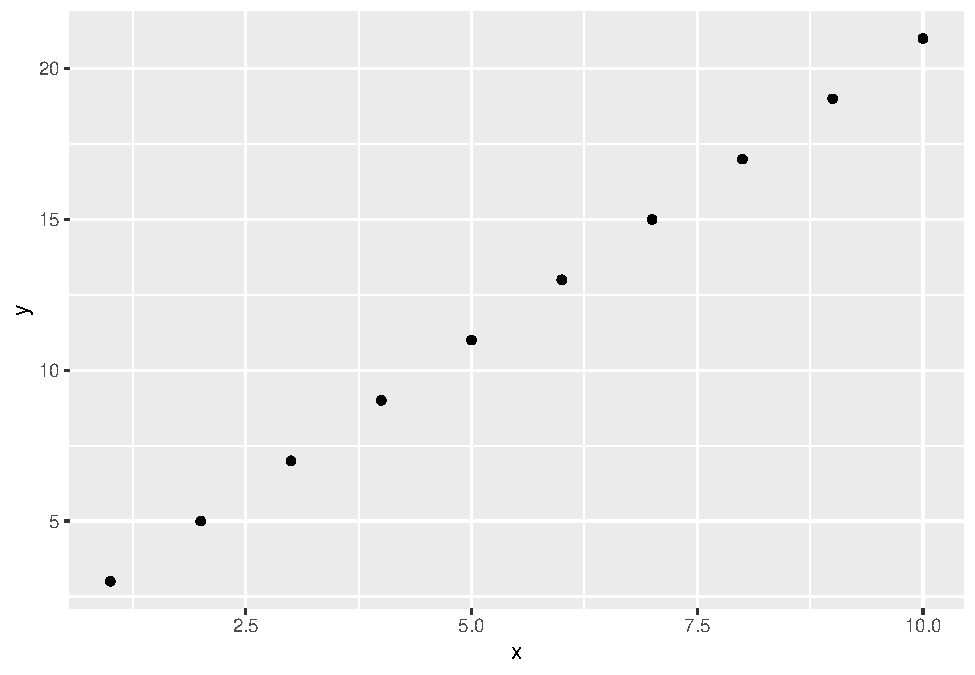
\includegraphics{main_files/figure-latex/unnamed-chunk-36-1.pdf}

Let us now plot a line to make our plot more informative and better looking.

\begin{Shaded}
\begin{Highlighting}[]
\CommentTok{\# Let us now plot x and y using ggplot2}
\FunctionTok{ggplot}\NormalTok{(}\AttributeTok{data=}\ConstantTok{NULL}\NormalTok{, }\FunctionTok{aes}\NormalTok{(x,y)) }\SpecialCharTok{+}
  \FunctionTok{geom\_point}\NormalTok{() }\SpecialCharTok{+}
  \FunctionTok{geom\_smooth}\NormalTok{(}\AttributeTok{method=}\StringTok{"lm"}\NormalTok{)}
\end{Highlighting}
\end{Shaded}

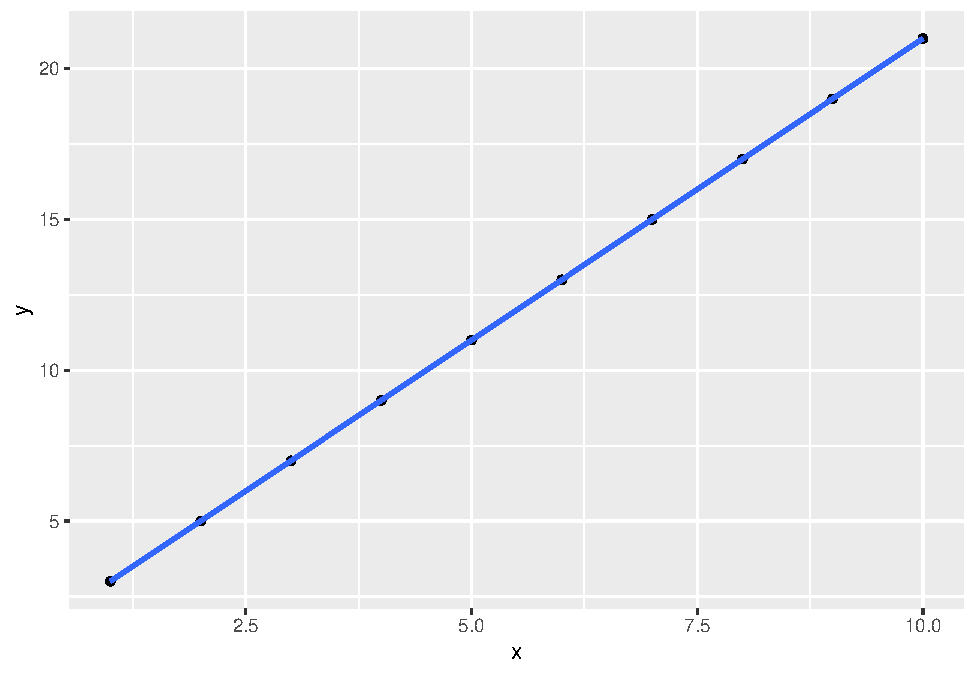
\includegraphics{main_files/figure-latex/unnamed-chunk-37-1.pdf}

Notice that playing with the scale sizes will yield dramatic changes in the effects we observe. For this, we can simply use the \texttt{xlim()} and \texttt{ylim()} functions to identify the lower and upper limits of x and y axes.

\begin{Shaded}
\begin{Highlighting}[]
\FunctionTok{ggplot}\NormalTok{(}\AttributeTok{data=}\ConstantTok{NULL}\NormalTok{, }\FunctionTok{aes}\NormalTok{(x,y)) }\SpecialCharTok{+}
  \FunctionTok{geom\_point}\NormalTok{() }\SpecialCharTok{+}
  \FunctionTok{geom\_smooth}\NormalTok{(}\AttributeTok{method=}\StringTok{"lm"}\NormalTok{)}\SpecialCharTok{+}
  \FunctionTok{xlim}\NormalTok{(}\DecValTok{0}\NormalTok{, }\DecValTok{15}\NormalTok{) }\SpecialCharTok{+}
  \FunctionTok{ylim}\NormalTok{(}\DecValTok{0}\NormalTok{,}\DecValTok{100}\NormalTok{)}
\end{Highlighting}
\end{Shaded}

\begin{verbatim}
## `geom_smooth()` using formula 'y ~ x'
\end{verbatim}

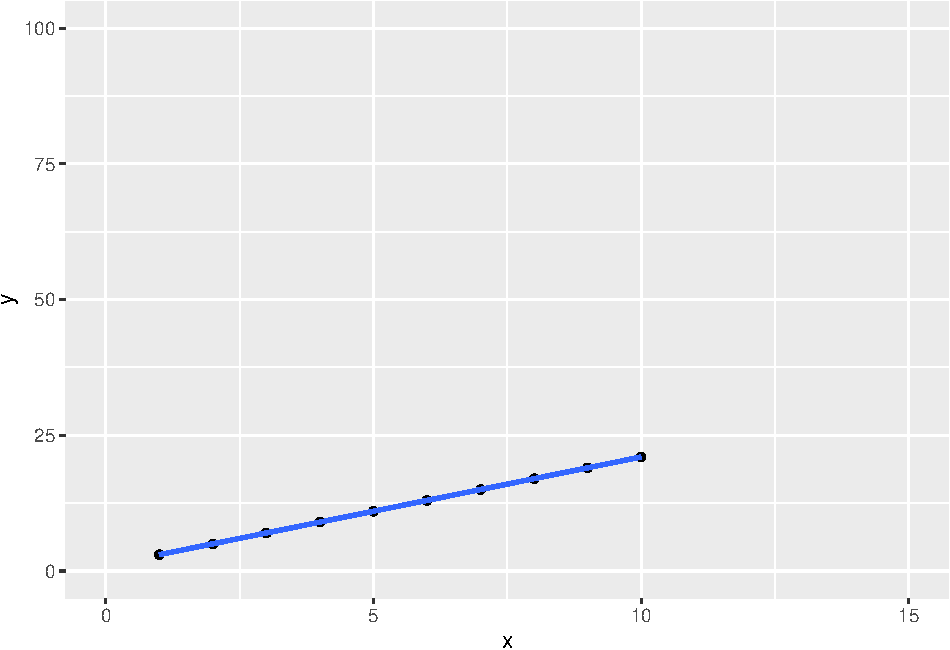
\includegraphics{main_files/figure-latex/unnamed-chunk-38-1.pdf}

Let us now plot a quadratic function. A quadratic function is one where the base is a variable and the exponent is constant. The following graph plots \texttt{n\^{}2}.

\begin{Shaded}
\begin{Highlighting}[]
\CommentTok{\# Let us now plot a and b using ggplot2}

\NormalTok{a}\OtherTok{\textless{}{-}} \DecValTok{1}\SpecialCharTok{:}\DecValTok{10}
\NormalTok{b }\OtherTok{\textless{}{-}}\NormalTok{ a}\SpecialCharTok{\^{}}\DecValTok{2}
\FunctionTok{ggplot}\NormalTok{(}\AttributeTok{data=}\ConstantTok{NULL}\NormalTok{, }\FunctionTok{aes}\NormalTok{(a,b)) }\SpecialCharTok{+}
  \FunctionTok{geom\_point}\NormalTok{() }\SpecialCharTok{+}
  \FunctionTok{geom\_smooth}\NormalTok{(}\AttributeTok{method=}\StringTok{"lm"}\NormalTok{,}\AttributeTok{formula =}\NormalTok{ y}\SpecialCharTok{\textasciitilde{}}\NormalTok{x }\SpecialCharTok{+}\FunctionTok{I}\NormalTok{(x}\SpecialCharTok{\^{}}\DecValTok{2}\NormalTok{), }\AttributeTok{color=}\StringTok{\textquotesingle{}orange\textquotesingle{}}\NormalTok{)}
\end{Highlighting}
\end{Shaded}

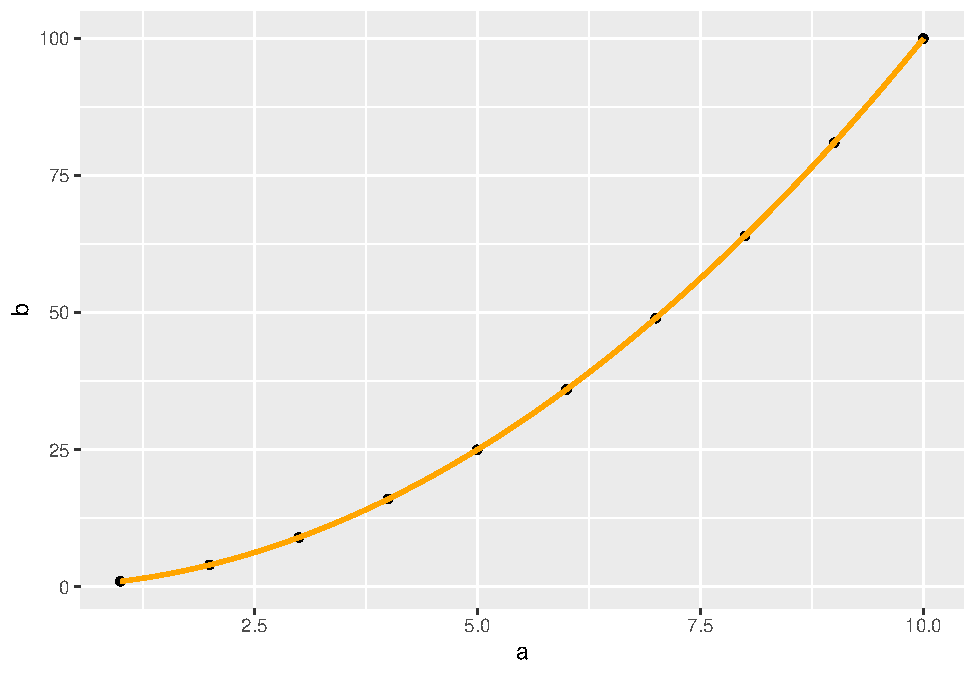
\includegraphics{main_files/figure-latex/unnamed-chunk-39-1.pdf}

Finally, we can plot an exponential function where the variable is the exponent and the base is constant.

\begin{Shaded}
\begin{Highlighting}[]
\CommentTok{\# Let us now plot a and b using ggplot2}

\NormalTok{a}\OtherTok{\textless{}{-}} \DecValTok{1}\SpecialCharTok{:}\DecValTok{10}
\NormalTok{b }\OtherTok{\textless{}{-}} \FunctionTok{exp}\NormalTok{(a)}
\FunctionTok{ggplot}\NormalTok{(}\AttributeTok{data=}\ConstantTok{NULL}\NormalTok{, }\FunctionTok{aes}\NormalTok{(a,b)) }\SpecialCharTok{+}
  \FunctionTok{geom\_point}\NormalTok{() }\SpecialCharTok{+}
  \FunctionTok{geom\_smooth}\NormalTok{(}\AttributeTok{method=}\StringTok{"lm"}\NormalTok{,}\AttributeTok{color =} \StringTok{"orange"}\NormalTok{,}\AttributeTok{formula=}\NormalTok{ (y }\SpecialCharTok{\textasciitilde{}} \FunctionTok{exp}\NormalTok{(x)))}
\end{Highlighting}
\end{Shaded}

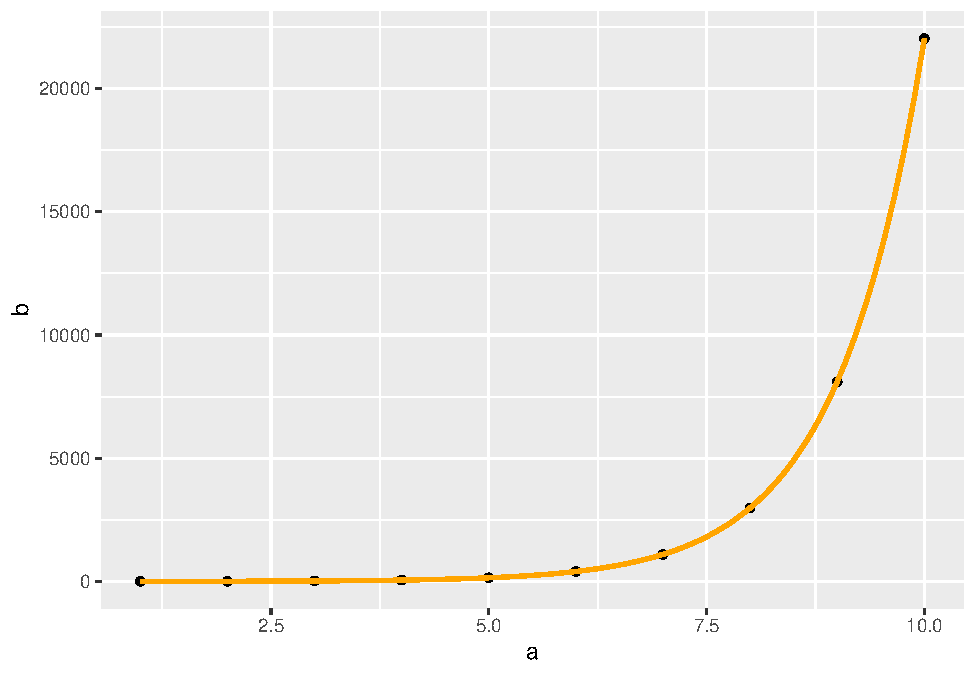
\includegraphics{main_files/figure-latex/unnamed-chunk-40-1.pdf}

You can mix and match.

\begin{Shaded}
\begin{Highlighting}[]
\CommentTok{\# Let us now plot x and y using ggplot2}
\NormalTok{a}\OtherTok{\textless{}{-}} \DecValTok{1}\SpecialCharTok{:}\DecValTok{10}
\NormalTok{b}\OtherTok{\textless{}{-}}\NormalTok{ a}\SpecialCharTok{\^{}}\DecValTok{2}
\FunctionTok{ggplot}\NormalTok{(}\AttributeTok{data=}\ConstantTok{NULL}\NormalTok{, }\FunctionTok{aes}\NormalTok{(x,y)) }\SpecialCharTok{+}
  \FunctionTok{geom\_smooth}\NormalTok{(}\AttributeTok{method=}\StringTok{"lm"}\NormalTok{) }\SpecialCharTok{+}
  \FunctionTok{geom\_smooth}\NormalTok{(}\AttributeTok{data=}\ConstantTok{NULL}\NormalTok{, }\FunctionTok{aes}\NormalTok{(a,b), }\AttributeTok{method=}\StringTok{"lm"}\NormalTok{, }\AttributeTok{formula =}\NormalTok{ y}\SpecialCharTok{\textasciitilde{}}\NormalTok{x }\SpecialCharTok{+}\FunctionTok{I}\NormalTok{(x}\SpecialCharTok{\^{}}\DecValTok{2}\NormalTok{),}\AttributeTok{color=} \StringTok{\textquotesingle{}orange\textquotesingle{}}\NormalTok{) }
\end{Highlighting}
\end{Shaded}

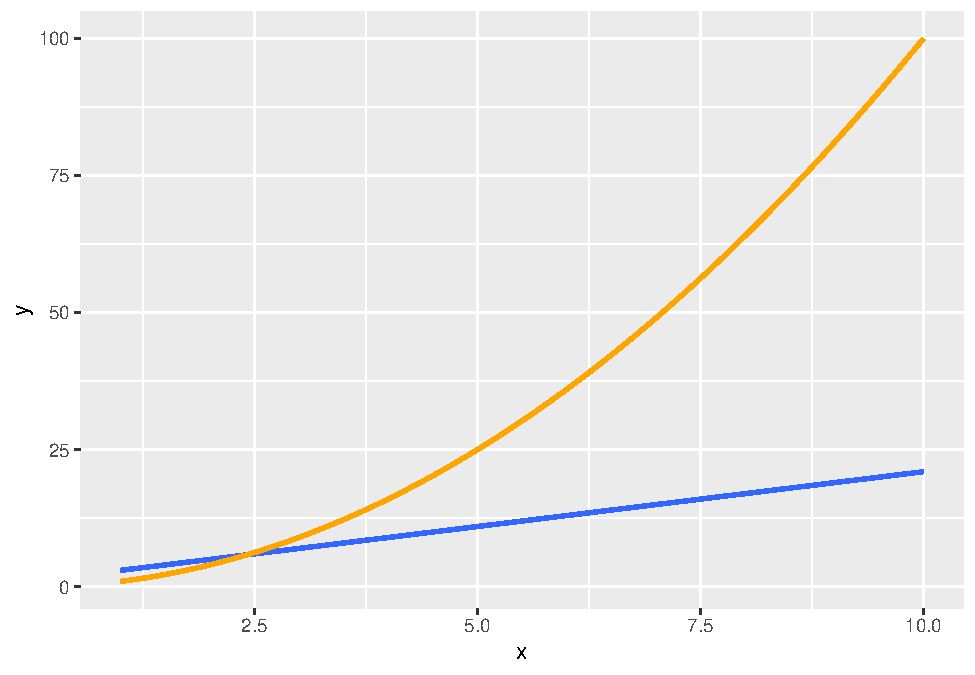
\includegraphics{main_files/figure-latex/unnamed-chunk-41-1.pdf}

\hypertarget{operators-and-functions-in-this-section}{%
\section{Operators and functions in this section}\label{operators-and-functions-in-this-section}}

\hypertarget{operators-1}{%
\subsection{Operators}\label{operators-1}}

\texttt{x\ +\ y}

Addition

\texttt{x\ -\ y}

Subtraction

\texttt{x\ *\ y}

Multiplication

\texttt{x\ /\ y}

Division

\texttt{x\^{}y}

Exponentiation

\texttt{x\ \textless{}-\ y}

Assignment

\texttt{==}

Test for equality. \textbf{Don't confuse with a single =, which is an assignment operator (and also always returns TRUE).}

\texttt{!=}

Test for inequality

\texttt{\textless{}}

Test, smaller than

\texttt{\textgreater{}}

Test, greater than

\texttt{\textless{}=}

Test, smaller than or equal to

\texttt{\textgreater{}=}

Test, greater than or equal to

\hypertarget{functions}{%
\subsection{Functions}\label{functions}}

\texttt{install.packages(package\_name)}

Installs one or several package(s).
The argument \texttt{package\_name} can either be a character (\texttt{install.packages(\textquotesingle{}dplyr\textquotesingle{})}) like or a character vector (\texttt{install.packages(c(\textquotesingle{}dplyr\textquotesingle{},\textquotesingle{}ggplot2\textquotesingle{}))}).

\texttt{library(package\_name)}

Loads a package called \texttt{package\_name}.

\hfill\break

\texttt{typeof(x)}

Determines the type of a variable/vector.

\hfill\break

\texttt{as.double(x)}

Converts a variable/vector to type \textbf{double}.

\hypertarget{data-structures}{%
\chapter{Data Structures}\label{data-structures}}

\hypertarget{data-types-in-r}{%
\section{Data Types in R}\label{data-types-in-r}}

In R, value has a \emph{type}:

\begin{longtable}[]{@{}
  >{\raggedleft\arraybackslash}p{(\columnwidth - 2\tabcolsep) * \real{0.2667}}
  >{\centering\arraybackslash}p{(\columnwidth - 2\tabcolsep) * \real{0.7333}}@{}}
\toprule()
\begin{minipage}[b]{\linewidth}\raggedleft
Data Type
\end{minipage} & \begin{minipage}[b]{\linewidth}\centering
Examples
\end{minipage} \\
\midrule()
\endhead
Integer (Numeric): & \ldots, -3, -2, -1, 0, +1, +2, +3, \ldots{} \\
Double (Numeric): & most rational numbers; e.g., 1.0, 1.5, 20.0, pi \\
Character: & \texttt{"a"}, \texttt{"b"}, \texttt{"word"}, \texttt{"hello\ dear\ friend,\ ..."} \\
Logical: & \texttt{TRUE} or \texttt{FALSE} (or: \texttt{T} or \texttt{F} ) \\
Factor: & Restricted, user-defined set of values, internally represented numerically (e.g., Gender \{`male', `female', `other'\}) \\
Ordered factor: & Factor with an ordering (e.g., Starbucks coffee sizes \{`venti' \textgreater{} `grande' \textgreater{} `tall'\}) \\
\bottomrule()
\end{longtable}

\hypertarget{data-structures-in-r}{%
\section{Data Structures in R}\label{data-structures-in-r}}

\begin{itemize}
\item
  All values in R are organized in data structures. Structures differ in their number of dimensions and in whether they allow mixed data types.
\item
  In this course, we will mainly use vectors and data frames.
\end{itemize}

\begin{longtable}[]{@{}
  >{\raggedleft\arraybackslash}p{(\columnwidth - 6\tabcolsep) * \real{0.1667}}
  >{\centering\arraybackslash}p{(\columnwidth - 6\tabcolsep) * \real{0.3571}}
  >{\centering\arraybackslash}p{(\columnwidth - 6\tabcolsep) * \real{0.2381}}
  >{\centering\arraybackslash}p{(\columnwidth - 6\tabcolsep) * \real{0.2381}}@{}}
\toprule()
\begin{minipage}[b]{\linewidth}\raggedleft
\end{minipage} & \begin{minipage}[b]{\linewidth}\centering
dimensions
\end{minipage} & \begin{minipage}[b]{\linewidth}\centering
types
\end{minipage} & \begin{minipage}[b]{\linewidth}\centering
\end{minipage} \\
\midrule()
\endhead
Vector & 1-dimensional & one type & 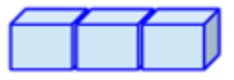
\includegraphics[width=0.25\textwidth,height=\textheight]{img/vector.jpg} \\
Matrix & 2-dimensional & one type & 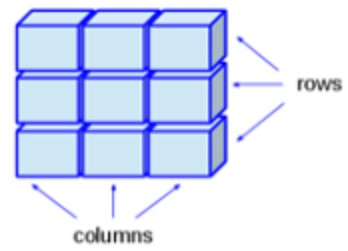
\includegraphics[width=0.2\textwidth,height=\textheight]{img/matrix.jpg} \\
Array & n-dimensional & one type & 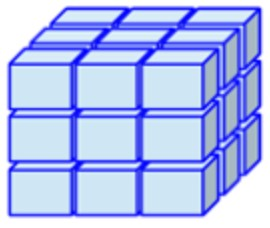
\includegraphics[width=0.2\textwidth,height=\textheight]{img/array.jpg} \\
Data frame (or tibble) & 2-dimensional & mixed types & 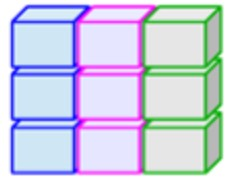
\includegraphics[width=0.2\textwidth,height=\textheight]{img/data_frame.jpg} \\
List & 1-dimensional & mixed types & 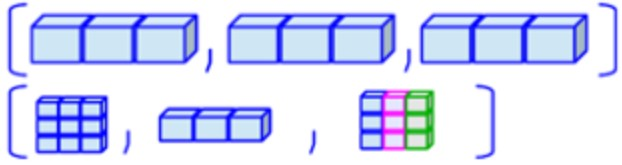
\includegraphics[width=0.5\textwidth,height=\textheight]{img/list.jpg} \\
\bottomrule()
\end{longtable}

(Illustrations from Gaurav Tiwari's article on medium \href{https://medium.com/@tiwarigaurav2512/r-data-types-847fffb01d5b}{here}.)

\begin{itemize}
\tightlist
\item
  Let's look at some examples
\end{itemize}

\begin{Shaded}
\begin{Highlighting}[]
\CommentTok{\# create and print vectors, don\textquotesingle{}t save}
\FunctionTok{c}\NormalTok{(}\DecValTok{1}\NormalTok{,}\DecValTok{2}\NormalTok{, }\DecValTok{1000}\NormalTok{)}
\end{Highlighting}
\end{Shaded}

\begin{Shaded}
\begin{Highlighting}[]
\NormalTok{\#\# [1]    1    2 1000}
\end{Highlighting}
\end{Shaded}

\begin{Shaded}
\begin{Highlighting}[]
\FunctionTok{c}\NormalTok{(}\DecValTok{1}\NormalTok{,}\DecValTok{2}\NormalTok{, }\DecValTok{1000}\NormalTok{, pi)}
\end{Highlighting}
\end{Shaded}

\begin{Shaded}
\begin{Highlighting}[]
\NormalTok{\#\# [1]    1.000000    2.000000 1000.000000    3.141593}
\end{Highlighting}
\end{Shaded}

\begin{Shaded}
\begin{Highlighting}[]
\DecValTok{1}\SpecialCharTok{:}\DecValTok{3}
\end{Highlighting}
\end{Shaded}

\begin{Shaded}
\begin{Highlighting}[]
\NormalTok{\#\# [1] 1 2 3}
\end{Highlighting}
\end{Shaded}

\begin{Shaded}
\begin{Highlighting}[]
\CommentTok{\# create and print a data.frame}
\FunctionTok{data.frame}\NormalTok{(}\DecValTok{1}\SpecialCharTok{:}\DecValTok{3}\NormalTok{)}
\end{Highlighting}
\end{Shaded}

\begin{Shaded}
\begin{Highlighting}[]
\NormalTok{\#\#   X1.3}
\NormalTok{\#\# 1    1}
\NormalTok{\#\# 2    2}
\NormalTok{\#\# 3    3}
\end{Highlighting}
\end{Shaded}

\hypertarget{vectors}{%
\section{Vectors}\label{vectors}}

\begin{itemize}
\tightlist
\item
  Vectors are simply ordered lists of elements, where every element has the same type.
\item
  They are useful for storing sets or sequences of numbers.
\item
  Let's create a simple vector with all integers from 1 to 8 and look at its contents.
\end{itemize}

\begin{Shaded}
\begin{Highlighting}[]
\NormalTok{vector\_var }\OtherTok{\textless{}{-}} \FunctionTok{c}\NormalTok{(}\DecValTok{1}\NormalTok{,}\DecValTok{2}\NormalTok{,}\DecValTok{3}\NormalTok{,}\DecValTok{4}\NormalTok{,}\DecValTok{5}\NormalTok{,}\DecValTok{6}\NormalTok{,}\DecValTok{7}\NormalTok{,}\DecValTok{8}\NormalTok{)}
\NormalTok{vector\_var}
\end{Highlighting}
\end{Shaded}

\begin{Shaded}
\begin{Highlighting}[]
\NormalTok{\#\# [1] 1 2 3 4 5 6 7 8}
\end{Highlighting}
\end{Shaded}

\begin{itemize}
\tightlist
\item
  There is even a more elegant ways to do that:
\end{itemize}

\begin{Shaded}
\begin{Highlighting}[]
\NormalTok{vector\_var }\OtherTok{\textless{}{-}} \DecValTok{1}\SpecialCharTok{:}\DecValTok{8}
\NormalTok{vector\_var}
\end{Highlighting}
\end{Shaded}

\begin{Shaded}
\begin{Highlighting}[]
\NormalTok{\#\# [1] 1 2 3 4 5 6 7 8}
\end{Highlighting}
\end{Shaded}

\begin{itemize}
\tightlist
\item
  Now, let's create a simple vector with integers between 1 and 8, going in steps of 2.
\end{itemize}

\begin{Shaded}
\begin{Highlighting}[]
\NormalTok{vector\_var }\OtherTok{\textless{}{-}} \FunctionTok{seq}\NormalTok{(}\DecValTok{1}\NormalTok{,}\DecValTok{8}\NormalTok{, }\AttributeTok{by=}\DecValTok{2}\NormalTok{)}
\NormalTok{vector\_var}
\end{Highlighting}
\end{Shaded}

\begin{Shaded}
\begin{Highlighting}[]
\NormalTok{\#\# [1] 1 3 5 7}
\end{Highlighting}
\end{Shaded}

\begin{itemize}
\tightlist
\item
  Some useful vectors already exist in R.
\end{itemize}

\begin{Shaded}
\begin{Highlighting}[]
\NormalTok{letters}
\end{Highlighting}
\end{Shaded}

\begin{Shaded}
\begin{Highlighting}[]
\NormalTok{\#\#  [1] "a" "b" "c" "d" "e" "f" "g" "h" "i" "j" "k" "l" "m" "n" "o" "p" "q" "r" "s"}
\NormalTok{\#\# [20] "t" "u" "v" "w" "x" "y" "z"}
\end{Highlighting}
\end{Shaded}

\begin{Shaded}
\begin{Highlighting}[]
\NormalTok{LETTERS}
\end{Highlighting}
\end{Shaded}

\begin{Shaded}
\begin{Highlighting}[]
\NormalTok{\#\#  [1] "A" "B" "C" "D" "E" "F" "G" "H" "I" "J" "K" "L" "M" "N" "O" "P" "Q" "R" "S"}
\NormalTok{\#\# [20] "T" "U" "V" "W" "X" "Y" "Z"}
\end{Highlighting}
\end{Shaded}

\begin{itemize}
\tightlist
\item
  We can select specific elements of a vector by indexing it with \texttt{{[}{]}}.
\end{itemize}

\begin{Shaded}
\begin{Highlighting}[]
\CommentTok{\# the first letter}
\NormalTok{letters[}\DecValTok{1}\NormalTok{]}
\end{Highlighting}
\end{Shaded}

\begin{Shaded}
\begin{Highlighting}[]
\NormalTok{\#\# [1] "a"}
\end{Highlighting}
\end{Shaded}

\begin{Shaded}
\begin{Highlighting}[]
\CommentTok{\# the 13{-}th letter}
\NormalTok{letters[}\DecValTok{13}\NormalTok{]}
\end{Highlighting}
\end{Shaded}

\begin{Shaded}
\begin{Highlighting}[]
\NormalTok{\#\# [1] "m"}
\end{Highlighting}
\end{Shaded}

\begin{itemize}
\tightlist
\item
  Indices can be vectors too.
\end{itemize}

\begin{Shaded}
\begin{Highlighting}[]
\CommentTok{\# both of them}
\NormalTok{letters[}\FunctionTok{c}\NormalTok{(}\DecValTok{1}\NormalTok{,}\DecValTok{7}\NormalTok{)]}
\end{Highlighting}
\end{Shaded}

\begin{Shaded}
\begin{Highlighting}[]
\NormalTok{\#\# [1] "a" "g"}
\end{Highlighting}
\end{Shaded}

\begin{itemize}
\tightlist
\item
  We can even take a whole \emph{`slice'} of a vector.
\end{itemize}

\begin{Shaded}
\begin{Highlighting}[]
\CommentTok{\# both of them}
\NormalTok{letters[}\DecValTok{6}\SpecialCharTok{:}\DecValTok{12}\NormalTok{]}
\end{Highlighting}
\end{Shaded}

\begin{Shaded}
\begin{Highlighting}[]
\NormalTok{\#\# [1] "f" "g" "h" "i" "j" "k" "l"}
\end{Highlighting}
\end{Shaded}

\begin{itemize}
\tightlist
\item
  Indices can even be negative. A negative index \(-n\) means \emph{`everything' except \(n\)}.
\end{itemize}

\begin{Shaded}
\begin{Highlighting}[]
\CommentTok{\# both of them}
\NormalTok{letters[}\SpecialCharTok{{-}}\DecValTok{1}\NormalTok{]}
\end{Highlighting}
\end{Shaded}

\begin{Shaded}
\begin{Highlighting}[]
\NormalTok{\#\#  [1] "b" "c" "d" "e" "f" "g" "h" "i" "j" "k" "l" "m" "n" "o" "p" "q" "r" "s" "t"}
\NormalTok{\#\# [20] "u" "v" "w" "x" "y" "z"}
\end{Highlighting}
\end{Shaded}

\begin{itemize}
\tightlist
\item
  Vectors can be named.
\end{itemize}

\begin{Shaded}
\begin{Highlighting}[]
\NormalTok{digits }\OtherTok{\textless{}{-}} \FunctionTok{c}\NormalTok{(}\StringTok{\textquotesingle{}one\textquotesingle{}}\OtherTok{=}\DecValTok{1}\NormalTok{, }\StringTok{\textquotesingle{}two\textquotesingle{}}\OtherTok{=}\DecValTok{2}\NormalTok{, }\StringTok{\textquotesingle{}three\textquotesingle{}}\OtherTok{=}\DecValTok{3}\NormalTok{, }\StringTok{\textquotesingle{}four\textquotesingle{}}\OtherTok{=}\DecValTok{4}\NormalTok{, }\StringTok{\textquotesingle{}five\textquotesingle{}}\OtherTok{=}\DecValTok{5}\NormalTok{, }\StringTok{\textquotesingle{}six\textquotesingle{}}\OtherTok{=}\DecValTok{6}\NormalTok{)}
\end{Highlighting}
\end{Shaded}

\begin{itemize}
\tightlist
\item
  In this case, we can index by the name
\end{itemize}

\begin{Shaded}
\begin{Highlighting}[]
\NormalTok{digits[}\FunctionTok{c}\NormalTok{(}\StringTok{\textquotesingle{}one\textquotesingle{}}\NormalTok{, }\StringTok{\textquotesingle{}six\textquotesingle{}}\NormalTok{)]}
\end{Highlighting}
\end{Shaded}

\begin{Shaded}
\begin{Highlighting}[]
\NormalTok{\#\# one six }
\NormalTok{\#\#   1   6}
\end{Highlighting}
\end{Shaded}

\begin{itemize}
\tightlist
\item
  Believe it or not, everything in R is actually a vector. For example \texttt{9} is a vector with only one element, which is \texttt{9}.
\end{itemize}

\begin{Shaded}
\begin{Highlighting}[]
\DecValTok{9}
\end{Highlighting}
\end{Shaded}

\begin{Shaded}
\begin{Highlighting}[]
\NormalTok{\#\# [1] 9}
\end{Highlighting}
\end{Shaded}

\begin{itemize}
\tightlist
\item
  This is why every output begins with \texttt{{[}1{]}}. R tries to help you find numbers in printed vectors. Every time a vector is printed, it reminds you at which position in the vector we are.
\item
  The \texttt{{[}1{]}} in the output below tells you that \texttt{"a"} is the first element, and the \texttt{{[}20{]}} tells you that \texttt{"t"} is the 20-th element.
\end{itemize}

\begin{Shaded}
\begin{Highlighting}[]
\NormalTok{letters }\CommentTok{\# print a vector with all lower{-}case letters}
\end{Highlighting}
\end{Shaded}

\begin{Shaded}
\begin{Highlighting}[]
\NormalTok{\#\#  [1] "a" "b" "c" "d" "e" "f" "g" "h" "i" "j" "k" "l" "m" "n" "o" "p" "q" "r" "s"}
\NormalTok{\#\# [20] "t" "u" "v" "w" "x" "y" "z"}
\end{Highlighting}
\end{Shaded}

\hypertarget{what-are-vectors-good-for}{%
\subsection{What are vectors good for?}\label{what-are-vectors-good-for}}

\begin{itemize}
\tightlist
\item
  Let's put this knowledge to use.
\item
  Here are two vectors representing the winnings from my recent gambling:
\end{itemize}

\begin{Shaded}
\begin{Highlighting}[]
\NormalTok{horse\_bets\_payout\_tl }\OtherTok{\textless{}{-}} \FunctionTok{c}\NormalTok{(}\DecValTok{100}\NormalTok{, }\SpecialCharTok{{-}}\DecValTok{50}\NormalTok{, }\DecValTok{1}\NormalTok{, }\DecValTok{100}\NormalTok{, }\SpecialCharTok{{-}}\DecValTok{10}\NormalTok{, }\SpecialCharTok{{-}}\DecValTok{20}\NormalTok{, }\DecValTok{250}\NormalTok{, }\SpecialCharTok{{-}}\DecValTok{40}\NormalTok{, }\SpecialCharTok{{-}}\DecValTok{30}\NormalTok{, }\DecValTok{23}\NormalTok{, }\SpecialCharTok{{-}}\DecValTok{23}\NormalTok{, }\DecValTok{55}\NormalTok{, }\DecValTok{14}\NormalTok{, }\DecValTok{8}\NormalTok{, }\DecValTok{24}\NormalTok{, }\SpecialCharTok{{-}}\DecValTok{3}\NormalTok{)}
\end{Highlighting}
\end{Shaded}

\begin{Shaded}
\begin{Highlighting}[]
\NormalTok{poker\_payout\_tl }\OtherTok{\textless{}{-}} \FunctionTok{c}\NormalTok{(}\DecValTok{24}\NormalTok{, }\DecValTok{5}\NormalTok{, }\SpecialCharTok{{-}}\FloatTok{38.1}\NormalTok{, }\DecValTok{12}\NormalTok{, }\DecValTok{103}\NormalTok{, }\DecValTok{15}\NormalTok{, }\DecValTok{5}\NormalTok{, }\DecValTok{187}\NormalTok{, }\DecValTok{13}\NormalTok{, }\SpecialCharTok{{-}}\DecValTok{23}\NormalTok{, }\SpecialCharTok{{-}}\DecValTok{45}\NormalTok{, }\DecValTok{36}\NormalTok{)}
\end{Highlighting}
\end{Shaded}

\begin{itemize}
\tightlist
\item
  Let's find out which game is more profitable.
\item
  To get our average profit, we first need to compute the sum of a vector.
\item
  Then, we will divide the sum by the length of the vector.
\item
  First, let's compute the sums of these vectors.
\end{itemize}

\begin{Shaded}
\begin{Highlighting}[]
\FunctionTok{sum}\NormalTok{(horse\_bets\_payout\_tl)}
\end{Highlighting}
\end{Shaded}

\begin{Shaded}
\begin{Highlighting}[]
\NormalTok{\#\# [1] 399}
\end{Highlighting}
\end{Shaded}

\begin{Shaded}
\begin{Highlighting}[]
\FunctionTok{sum}\NormalTok{(poker\_payout\_tl)}
\end{Highlighting}
\end{Shaded}

\begin{Shaded}
\begin{Highlighting}[]
\NormalTok{\#\# [1] 293.9}
\end{Highlighting}
\end{Shaded}

\begin{itemize}
\tightlist
\item
  Now, we need to determine the length of these vectors:
\end{itemize}

\begin{Shaded}
\begin{Highlighting}[]
\FunctionTok{length}\NormalTok{(horse\_bets\_payout\_tl)}
\end{Highlighting}
\end{Shaded}

\begin{Shaded}
\begin{Highlighting}[]
\NormalTok{\#\# [1] 16}
\end{Highlighting}
\end{Shaded}

\begin{Shaded}
\begin{Highlighting}[]
\FunctionTok{length}\NormalTok{(poker\_payout\_tl)}
\end{Highlighting}
\end{Shaded}

\begin{Shaded}
\begin{Highlighting}[]
\NormalTok{\#\# [1] 12}
\end{Highlighting}
\end{Shaded}

\begin{itemize}
\tightlist
\item
  Dividing the sum by the length would give us our average profit.
\end{itemize}

\begin{Shaded}
\begin{Highlighting}[]
\FunctionTok{sum}\NormalTok{(horse\_bets\_payout\_tl)}\SpecialCharTok{/}\FunctionTok{length}\NormalTok{(horse\_bets\_payout\_tl)}
\end{Highlighting}
\end{Shaded}

\begin{Shaded}
\begin{Highlighting}[]
\NormalTok{\#\# [1] 24.9375}
\end{Highlighting}
\end{Shaded}

\begin{Shaded}
\begin{Highlighting}[]
\FunctionTok{sum}\NormalTok{(poker\_payout\_tl)}\SpecialCharTok{/}\FunctionTok{length}\NormalTok{(poker\_payout\_tl)}
\end{Highlighting}
\end{Shaded}

\begin{Shaded}
\begin{Highlighting}[]
\NormalTok{\#\# [1] 24.49167}
\end{Highlighting}
\end{Shaded}

\ldots{} so which game is more profitable?

\begin{itemize}
\item
  It seems that betting is more profitable.
\item
  Next time, we can accomplish this calulation by calling the function \texttt{mean()}.
\end{itemize}

\begin{Shaded}
\begin{Highlighting}[]
\FunctionTok{mean}\NormalTok{(horse\_bets\_payout\_tl)}
\end{Highlighting}
\end{Shaded}

\begin{Shaded}
\begin{Highlighting}[]
\NormalTok{\#\# [1] 24.9375}
\end{Highlighting}
\end{Shaded}

\begin{Shaded}
\begin{Highlighting}[]
\FunctionTok{mean}\NormalTok{(poker\_payout\_tl)}
\end{Highlighting}
\end{Shaded}

\begin{Shaded}
\begin{Highlighting}[]
\NormalTok{\#\# [1] 24.49167}
\end{Highlighting}
\end{Shaded}

\ldots Now, I forgot to mention that my bookie charges me 1.5 TL per bet on a horse, on average. The poker payouts correspond to the profits, though. \ldots 

\begin{itemize}
\item
  Luckily, we can just add numbers and vectors. Let's just create two new vectors which contain the profits.
\item
  Let's subtract 1.5 from elements of \texttt{horse\_bets\_payout\_tl} and save the result as \texttt{horse\_bets\_profits\_tl}.
\item
  As you see, this subtraction is applied to every element of the vector.
\end{itemize}

\begin{Shaded}
\begin{Highlighting}[]
\NormalTok{horse\_bets\_profits\_tl }\OtherTok{\textless{}{-}}\NormalTok{ horse\_bets\_payout\_tl }\SpecialCharTok{{-}} \FloatTok{1.5}
\FunctionTok{head}\NormalTok{(horse\_bets\_profits\_tl)}
\end{Highlighting}
\end{Shaded}

\begin{Shaded}
\begin{Highlighting}[]
\NormalTok{\#\# [1]  98.5 {-}51.5  {-}0.5  98.5 {-}11.5 {-}21.5}
\end{Highlighting}
\end{Shaded}

\begin{Shaded}
\begin{Highlighting}[]
\FunctionTok{head}\NormalTok{(horse\_bets\_payout\_tl)}
\end{Highlighting}
\end{Shaded}

\begin{Shaded}
\begin{Highlighting}[]
\NormalTok{\#\# [1] 100 {-}50   1 100 {-}10 {-}20}
\end{Highlighting}
\end{Shaded}

\begin{itemize}
\tightlist
\item
  For poker, we don't need to change anything. So, we assign the already existing \texttt{poker\_payout\_tl} vector to another vector called \texttt{poker\_profits\_tl}.
\end{itemize}

\begin{Shaded}
\begin{Highlighting}[]
\NormalTok{poker\_profits\_tl }\OtherTok{\textless{}{-}}\NormalTok{ poker\_payout\_tl}
\end{Highlighting}
\end{Shaded}

\begin{itemize}
\tightlist
\item
  Let's compare:
\end{itemize}

\begin{Shaded}
\begin{Highlighting}[]
\NormalTok{horse\_bets\_payout\_tl}
\end{Highlighting}
\end{Shaded}

\begin{Shaded}
\begin{Highlighting}[]
\NormalTok{\#\#  [1] 100 {-}50   1 100 {-}10 {-}20 250 {-}40 {-}30  23 {-}23  55  14   8  24  {-}3}
\end{Highlighting}
\end{Shaded}

\begin{Shaded}
\begin{Highlighting}[]
\NormalTok{horse\_bets\_profits\_tl}
\end{Highlighting}
\end{Shaded}

\begin{Shaded}
\begin{Highlighting}[]
\NormalTok{\#\#  [1]  98.5 {-}51.5  {-}0.5  98.5 {-}11.5 {-}21.5 248.5 {-}41.5 {-}31.5  21.5 {-}24.5  53.5}
\NormalTok{\#\# [13]  12.5   6.5  22.5  {-}4.5}
\end{Highlighting}
\end{Shaded}

\begin{Shaded}
\begin{Highlighting}[]
\NormalTok{poker\_payout\_tl}
\end{Highlighting}
\end{Shaded}

\begin{Shaded}
\begin{Highlighting}[]
\NormalTok{\#\#  [1]  24.0   5.0 {-}38.1  12.0 103.0  15.0   5.0 187.0  13.0 {-}23.0 {-}45.0  36.0}
\end{Highlighting}
\end{Shaded}

\begin{Shaded}
\begin{Highlighting}[]
\NormalTok{poker\_profits\_tl}
\end{Highlighting}
\end{Shaded}

\begin{Shaded}
\begin{Highlighting}[]
\NormalTok{\#\#  [1]  24.0   5.0 {-}38.1  12.0 103.0  15.0   5.0 187.0  13.0 {-}23.0 {-}45.0  36.0}
\end{Highlighting}
\end{Shaded}

\begin{itemize}
\tightlist
\item
  Which game is more profitable now?
\end{itemize}

\begin{Shaded}
\begin{Highlighting}[]
\FunctionTok{mean}\NormalTok{(horse\_bets\_profits\_tl)}
\end{Highlighting}
\end{Shaded}

\begin{Shaded}
\begin{Highlighting}[]
\NormalTok{\#\# [1] 23.4375}
\end{Highlighting}
\end{Shaded}

\begin{Shaded}
\begin{Highlighting}[]
\FunctionTok{mean}\NormalTok{(poker\_profits\_tl)}
\end{Highlighting}
\end{Shaded}

\begin{Shaded}
\begin{Highlighting}[]
\NormalTok{\#\# [1] 24.49167}
\end{Highlighting}
\end{Shaded}

\hypertarget{data-frames}{%
\section{Data Frames}\label{data-frames}}

\begin{itemize}
\tightlist
\item
  What I forgot to mention is that I generally gamble on Wednesdays and Fridays. Maybe that matters?
\item
  How can we associate this information with the profits vectors?
\end{itemize}

\begin{itemize}
\tightlist
\item
  One way is to represent it in two vectors containing days of the week. In that case, every \(i\)-th element in \texttt{poker\_week\_days} corresponds to the \(i\)-th element in \texttt{poker\_week\_days}.
\end{itemize}

\begin{Shaded}
\begin{Highlighting}[]
\CommentTok{\# create two vectors with week days}
\NormalTok{horse\_bets\_week\_days }\OtherTok{\textless{}{-}} \FunctionTok{rep}\NormalTok{(}\FunctionTok{c}\NormalTok{(}\StringTok{"Wed"}\NormalTok{, }\StringTok{"Fr"}\NormalTok{), }\DecValTok{8}\NormalTok{)}
\NormalTok{poker\_week\_days }\OtherTok{\textless{}{-}} \FunctionTok{rep}\NormalTok{(}\FunctionTok{c}\NormalTok{(}\StringTok{"Wed"}\NormalTok{, }\StringTok{"Fr"}\NormalTok{), }\DecValTok{6}\NormalTok{)}
\end{Highlighting}
\end{Shaded}

\begin{itemize}
\item
  But this is getting messy. We have to keep track of two pairs a vectors, and the relations between them. Let's represent all poker-related information in one data structure, and all horse race-related information in another structure.
\item
  The best way to represent a pair of vectors where the \(i\)-th element in vector 1 corresponds to the \(i\)-th element in vector 2 is with data frames. We can create a new data frame with the function \texttt{data.frame()}.
\end{itemize}

\begin{Shaded}
\begin{Highlighting}[]
\NormalTok{df\_horse\_bets }\OtherTok{\textless{}{-}} 
  \FunctionTok{data.frame}\NormalTok{(}\AttributeTok{wday =}\NormalTok{ horse\_bets\_week\_days, }
             \AttributeTok{profit =}\NormalTok{ horse\_bets\_profits\_tl)}
\end{Highlighting}
\end{Shaded}

\begin{Shaded}
\begin{Highlighting}[]
\NormalTok{df\_poker }\OtherTok{\textless{}{-}} 
  \FunctionTok{data.frame}\NormalTok{(}\AttributeTok{wday =}\NormalTok{ poker\_week\_days, }
             \AttributeTok{profit =}\NormalTok{ poker\_payout\_tl)}
\end{Highlighting}
\end{Shaded}

\begin{itemize}
\tightlist
\item
  Let's take a look at what we've created.
\end{itemize}

\begin{Shaded}
\begin{Highlighting}[]
\NormalTok{df\_horse\_bets}
\end{Highlighting}
\end{Shaded}

\begin{Shaded}
\begin{Highlighting}[]
\NormalTok{\#\#    wday profit}
\NormalTok{\#\# 1   Wed   98.5}
\NormalTok{\#\# 2    Fr  {-}51.5}
\NormalTok{\#\# 3   Wed   {-}0.5}
\NormalTok{\#\# 4    Fr   98.5}
\NormalTok{\#\# 5   Wed  {-}11.5}
\NormalTok{\#\# 6    Fr  {-}21.5}
\NormalTok{\#\# 7   Wed  248.5}
\NormalTok{\#\# 8    Fr  {-}41.5}
\NormalTok{\#\# 9   Wed  {-}31.5}
\NormalTok{\#\# 10   Fr   21.5}
\NormalTok{\#\# 11  Wed  {-}24.5}
\NormalTok{\#\# 12   Fr   53.5}
\NormalTok{\#\# 13  Wed   12.5}
\NormalTok{\#\# 14   Fr    6.5}
\NormalTok{\#\# 15  Wed   22.5}
\NormalTok{\#\# 16   Fr   {-}4.5}
\end{Highlighting}
\end{Shaded}

\begin{itemize}
\item
  Wow. That's a rather long output \ldots{}
\item
  Generally, it's sufficient to see the first couple of rows of a \texttt{data.frame} to get a sense of what it contains.
\item
  We'll use the function \texttt{head()}, which takes a \texttt{data.frame} and a number \(n\), and outputs the first \(n\) lines.
\end{itemize}

\begin{Shaded}
\begin{Highlighting}[]
\CommentTok{\# let\textquotesingle{}s see the first two rows of the data frame called df\_horse\_bets}
\FunctionTok{head}\NormalTok{(df\_horse\_bets, }\DecValTok{2}\NormalTok{) }
\end{Highlighting}
\end{Shaded}

\begin{Shaded}
\begin{Highlighting}[]
\NormalTok{\#\#   wday profit}
\NormalTok{\#\# 1  Wed   98.5}
\NormalTok{\#\# 2   Fr  {-}51.5}
\end{Highlighting}
\end{Shaded}

\begin{itemize}
\tightlist
\item
  An alternative is \texttt{View()}, which shows you the entire \texttt{data.frame} within a new tab in the RStudio GUI.
\end{itemize}

\begin{Shaded}
\begin{Highlighting}[]
\FunctionTok{View}\NormalTok{(df\_poker)}
\end{Highlighting}
\end{Shaded}

\begin{itemize}
\item
  Turning back to our gambling example, we still have two objects, which really belong together.
\item
  Let's merge them into one long data frame.
\item
  The function \texttt{rbind()} takes two data frames as its arguments, and returns a single concatenated data frame, where all the rows of the first data frame are on top, and all the rows of the second data frame are at the bottom.
\end{itemize}

\begin{Shaded}
\begin{Highlighting}[]
\NormalTok{df\_gambling }\OtherTok{\textless{}{-}} \FunctionTok{rbind}\NormalTok{(df\_horse\_bets, df\_poker)}
\end{Highlighting}
\end{Shaded}

\begin{itemize}
\tightlist
\item
  Unfortunately, now, we don't have any information on which profits are from which game.
\end{itemize}

\begin{Shaded}
\begin{Highlighting}[]
\FunctionTok{head}\NormalTok{(df\_gambling)}
\end{Highlighting}
\end{Shaded}

\begin{Shaded}
\begin{Highlighting}[]
\NormalTok{\#\#   wday profit}
\NormalTok{\#\# 1  Wed   98.5}
\NormalTok{\#\# 2   Fr  {-}51.5}
\NormalTok{\#\# 3  Wed   {-}0.5}
\NormalTok{\#\# 4   Fr   98.5}
\NormalTok{\#\# 5  Wed  {-}11.5}
\NormalTok{\#\# 6   Fr  {-}21.5}
\end{Highlighting}
\end{Shaded}

\begin{itemize}
\tightlist
\item
  Let's fix this problem by enriching both data frames with this information.
\item
  We can assign to new (or old) columns with our assignment operator \texttt{\textless{}-}.
\item
  When we assign a value to a specific column, R puts the specified value into every row of the column of the given data frame.
\item
  What the following code says is ``Create a new column named \texttt{game} in the data frame named \texttt{df\_horse\_bets} and fill the column with the string \emph{horse\_bets}.''
\end{itemize}

\begin{Shaded}
\begin{Highlighting}[]
\NormalTok{df\_horse\_bets}\SpecialCharTok{$}\NormalTok{game }\OtherTok{\textless{}{-}} \StringTok{"horse\_bets"}
\NormalTok{df\_poker}\SpecialCharTok{$}\NormalTok{game }\OtherTok{\textless{}{-}} \StringTok{"poker"}
\end{Highlighting}
\end{Shaded}

\begin{itemize}
\tightlist
\item
  Now, let's bind them together again. (This overwrites the old data frame called \texttt{df\_gambling}, which we created previously.)
\end{itemize}

\begin{Shaded}
\begin{Highlighting}[]
\NormalTok{df\_gambling }\OtherTok{\textless{}{-}} \FunctionTok{rbind}\NormalTok{(df\_horse\_bets, df\_poker)}
\FunctionTok{head}\NormalTok{(df\_gambling)}
\end{Highlighting}
\end{Shaded}

\begin{Shaded}
\begin{Highlighting}[]
\NormalTok{\#\#   wday profit       game}
\NormalTok{\#\# 1  Wed   98.5 horse\_bets}
\NormalTok{\#\# 2   Fr  {-}51.5 horse\_bets}
\NormalTok{\#\# 3  Wed   {-}0.5 horse\_bets}
\NormalTok{\#\# 4   Fr   98.5 horse\_bets}
\NormalTok{\#\# 5  Wed  {-}11.5 horse\_bets}
\NormalTok{\#\# 6   Fr  {-}21.5 horse\_bets}
\end{Highlighting}
\end{Shaded}

\hypertarget{working-with-data-frames}{%
\section{Working with data frames}\label{working-with-data-frames}}

\begin{itemize}
\tightlist
\item
  Now, we can do very cool things very easily.
\item
  But we'll need two packages for that: \texttt{dplyr}, and \texttt{magrittr}.
\end{itemize}

\begin{Shaded}
\begin{Highlighting}[]
\CommentTok{\# load the two packages}
\FunctionTok{library}\NormalTok{(magrittr) }\CommentTok{\# for \textquotesingle{}\%\textgreater{}\%\textquotesingle{}}
\end{Highlighting}
\end{Shaded}

\begin{verbatim}
## 
## Attaching package: 'magrittr'
\end{verbatim}

\begin{verbatim}
## The following object is masked from 'package:purrr':
## 
##     set_names
\end{verbatim}

\begin{verbatim}
## The following object is masked from 'package:tidyr':
## 
##     extract
\end{verbatim}

\begin{Shaded}
\begin{Highlighting}[]
\FunctionTok{library}\NormalTok{(dplyr) }\CommentTok{\# for group\_by() and summarize()}
\end{Highlighting}
\end{Shaded}

\begin{itemize}
\item
  Now, we can \emph{`aggregate'} data \emph{(= ``combine data from several measurements by replacing it by summary statistics'')}.
\item
  Let's compute the average profit by \texttt{game}.
\item
  Within the \texttt{summarize()} function, we specify new columns.
\item
  In this case, \texttt{avg\_profit} is the name of our column and its content is mean of the profit column.
\item
  Keep in mind that \texttt{summarize()} function is applied at the group level.
\end{itemize}

\begin{Shaded}
\begin{Highlighting}[]
\NormalTok{df\_gambling }\SpecialCharTok{\%\textgreater{}\%} 
  \FunctionTok{group\_by}\NormalTok{(game) }\SpecialCharTok{\%\textgreater{}\%} 
  \FunctionTok{summarize}\NormalTok{(}\AttributeTok{avg\_profit =} \FunctionTok{mean}\NormalTok{(profit))}
\end{Highlighting}
\end{Shaded}

\begin{Shaded}
\begin{Highlighting}[]
\NormalTok{\#\# \# A tibble: 2 x 2}
\NormalTok{\#\#   game       avg\_profit}
\NormalTok{\#\#   \textless{}chr\textgreater{}           \textless{}dbl\textgreater{}}
\NormalTok{\#\# 1 horse\_bets       23.4}
\NormalTok{\#\# 2 poker            24.5}
\end{Highlighting}
\end{Shaded}

\begin{itemize}
\tightlist
\item
  We can also aggregate over several grouping variables at the same time, like \texttt{game} and \texttt{wday}.
\end{itemize}

\begin{Shaded}
\begin{Highlighting}[]
\NormalTok{df\_gambling }\SpecialCharTok{\%\textgreater{}\%} 
  \FunctionTok{group\_by}\NormalTok{(game, wday) }\SpecialCharTok{\%\textgreater{}\%} 
  \FunctionTok{summarize}\NormalTok{(}\AttributeTok{avg\_profit =} \FunctionTok{mean}\NormalTok{(profit))}
\end{Highlighting}
\end{Shaded}

\begin{verbatim}
## `summarise()` has grouped output by 'game'. You can override using the
## `.groups` argument.
\end{verbatim}

\begin{Shaded}
\begin{Highlighting}[]
\NormalTok{\#\# \# A tibble: 4 x 3}
\NormalTok{\#\# \# Groups:   game [2]}
\NormalTok{\#\#   game       wday  avg\_profit}
\NormalTok{\#\#   \textless{}chr\textgreater{}      \textless{}chr\textgreater{}      \textless{}dbl\textgreater{}}
\NormalTok{\#\# 1 horse\_bets Fr          7.62}
\NormalTok{\#\# 2 horse\_bets Wed        39.2 }
\NormalTok{\#\# 3 poker      Fr         38.7 }
\NormalTok{\#\# 4 poker      Wed        10.3}
\end{Highlighting}
\end{Shaded}

\begin{itemize}
\tightlist
\item
  \ldots{} and we can do so in various ways. Here we compute the proportion of wins.
\end{itemize}

\begin{Shaded}
\begin{Highlighting}[]
\NormalTok{df\_gambling }\SpecialCharTok{\%\textgreater{}\%} 
  \FunctionTok{group\_by}\NormalTok{(game, wday) }\SpecialCharTok{\%\textgreater{}\%} 
  \FunctionTok{summarize}\NormalTok{(}\AttributeTok{avg\_proportion\_wins =} \FunctionTok{mean}\NormalTok{(profit}\SpecialCharTok{\textgreater{}}\DecValTok{0}\NormalTok{) )}
\end{Highlighting}
\end{Shaded}

\begin{verbatim}
## `summarise()` has grouped output by 'game'. You can override using the
## `.groups` argument.
\end{verbatim}

\begin{Shaded}
\begin{Highlighting}[]
\NormalTok{\#\# \# A tibble: 4 x 3}
\NormalTok{\#\# \# Groups:   game [2]}
\NormalTok{\#\#   game       wday  avg\_proportion\_wins}
\NormalTok{\#\#   \textless{}chr\textgreater{}      \textless{}chr\textgreater{}               \textless{}dbl\textgreater{}}
\NormalTok{\#\# 1 horse\_bets Fr                  0.5  }
\NormalTok{\#\# 2 horse\_bets Wed                 0.5  }
\NormalTok{\#\# 3 poker      Fr                  0.833}
\NormalTok{\#\# 4 poker      Wed                 0.667}
\end{Highlighting}
\end{Shaded}

\begin{itemize}
\tightlist
\item
  Now, we can also plot the results.
\item
  But we'll need to save the summary statistics first.
\end{itemize}

\begin{Shaded}
\begin{Highlighting}[]
\NormalTok{profits\_by\_game }\OtherTok{\textless{}{-}} 
\NormalTok{  df\_gambling }\SpecialCharTok{\%\textgreater{}\%} 
    \FunctionTok{group\_by}\NormalTok{(game) }\SpecialCharTok{\%\textgreater{}\%} 
    \FunctionTok{summarize}\NormalTok{(}\AttributeTok{avg\_profit =} \FunctionTok{mean}\NormalTok{(profit))}
\end{Highlighting}
\end{Shaded}

\begin{Shaded}
\begin{Highlighting}[]
\NormalTok{profits\_by\_game\_and\_wday }\OtherTok{\textless{}{-}} 
\NormalTok{  df\_gambling }\SpecialCharTok{\%\textgreater{}\%} 
    \FunctionTok{group\_by}\NormalTok{(game, wday) }\SpecialCharTok{\%\textgreater{}\%} 
    \FunctionTok{summarize}\NormalTok{(}\AttributeTok{avg\_profit =} \FunctionTok{mean}\NormalTok{(profit))}
\end{Highlighting}
\end{Shaded}

\begin{verbatim}
## `summarise()` has grouped output by 'game'. You can override using the
## `.groups` argument.
\end{verbatim}

\begin{itemize}
\tightlist
\item
  We will also need yet another package (for plotting): \texttt{ggplot2}.
\end{itemize}

\begin{Shaded}
\begin{Highlighting}[]
\FunctionTok{library}\NormalTok{(ggplot2)}
\end{Highlighting}
\end{Shaded}

\begin{itemize}
\tightlist
\item
  After loading the package ggplot2, we can create plots with the function \texttt{ggplot()}. We will be going over the details in the upcoming chapters.
\end{itemize}

\begin{Shaded}
\begin{Highlighting}[]
\FunctionTok{ggplot}\NormalTok{(profits\_by\_game, }\FunctionTok{aes}\NormalTok{(game, avg\_profit)) }\SpecialCharTok{+} \FunctionTok{geom\_point}\NormalTok{()}
\end{Highlighting}
\end{Shaded}

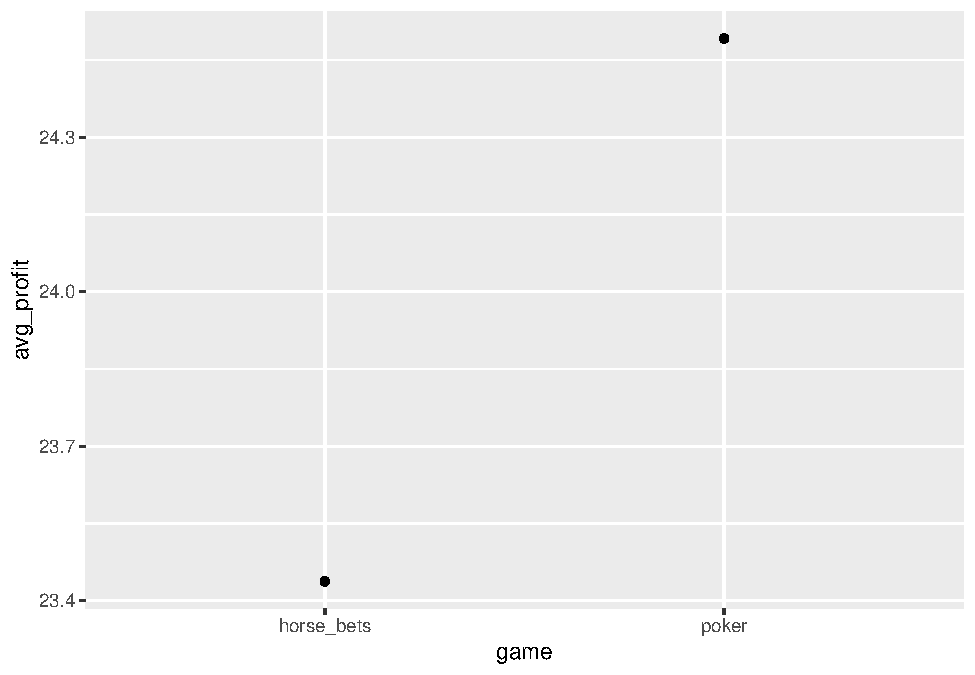
\includegraphics{main_files/figure-latex/unnamed-chunk-89-1.pdf}

\begin{itemize}
\tightlist
\item
  We may also want lines that connect the points.
\end{itemize}

\begin{Shaded}
\begin{Highlighting}[]
\FunctionTok{library}\NormalTok{(ggplot2)}
\FunctionTok{ggplot}\NormalTok{(profits\_by\_game\_and\_wday, }\FunctionTok{aes}\NormalTok{(game, avg\_profit, }\AttributeTok{color =}\NormalTok{ wday, }\AttributeTok{group =}\NormalTok{ wday)) }\SpecialCharTok{+} \FunctionTok{geom\_point}\NormalTok{() }\SpecialCharTok{+} \FunctionTok{geom\_line}\NormalTok{()}
\end{Highlighting}
\end{Shaded}

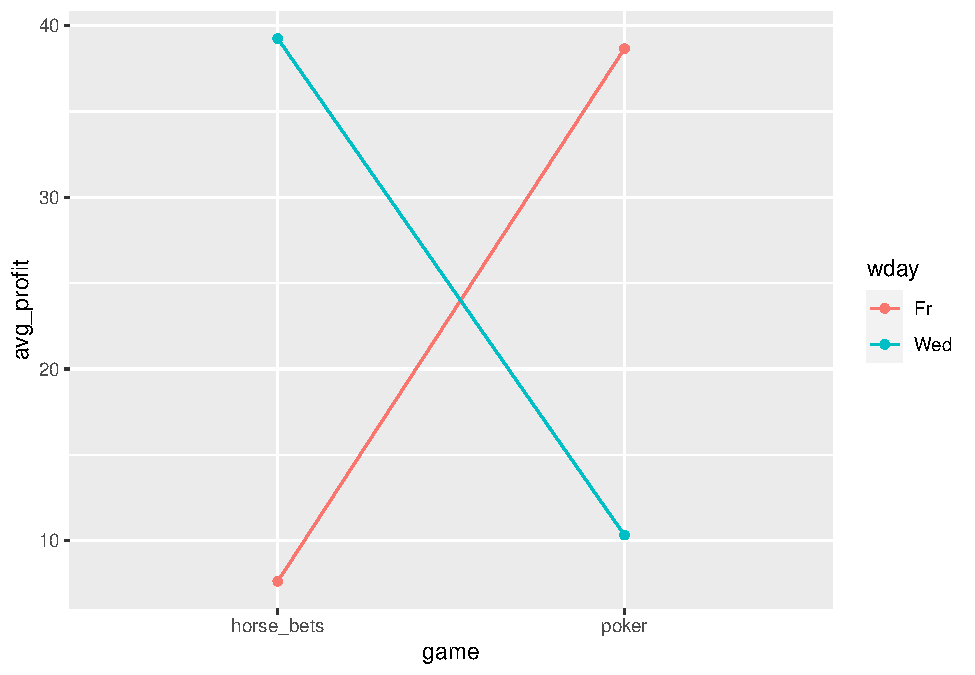
\includegraphics{main_files/figure-latex/unnamed-chunk-90-1.pdf}

\begin{itemize}
\tightlist
\item
  Or, we may want to have a bar graph.
\end{itemize}

\begin{Shaded}
\begin{Highlighting}[]
\FunctionTok{library}\NormalTok{(ggplot2)}
\FunctionTok{ggplot}\NormalTok{(profits\_by\_game, }\FunctionTok{aes}\NormalTok{(game, avg\_profit)) }\SpecialCharTok{+} \FunctionTok{geom\_bar}\NormalTok{(}\AttributeTok{stat =} \StringTok{"identity"}\NormalTok{)}
\end{Highlighting}
\end{Shaded}

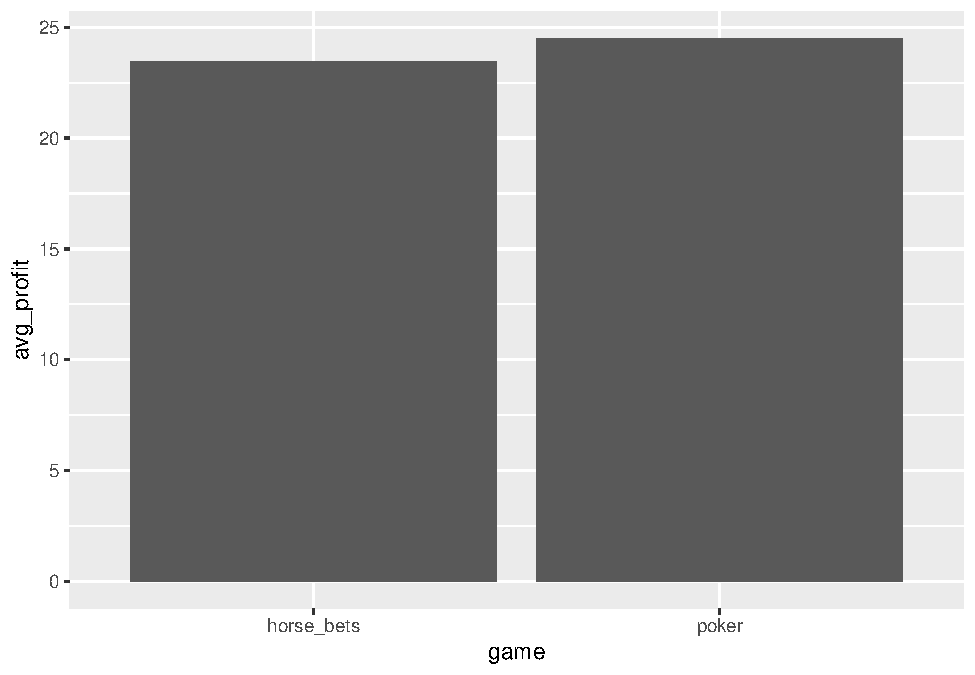
\includegraphics{main_files/figure-latex/unnamed-chunk-91-1.pdf}

\begin{Shaded}
\begin{Highlighting}[]
\FunctionTok{library}\NormalTok{(ggplot2)}
\FunctionTok{ggplot}\NormalTok{(profits\_by\_game\_and\_wday, }\FunctionTok{aes}\NormalTok{(game, avg\_profit, }\AttributeTok{fill =}\NormalTok{ wday)) }\SpecialCharTok{+} \FunctionTok{geom\_bar}\NormalTok{(}\AttributeTok{stat =} \StringTok{"identity"}\NormalTok{, }\AttributeTok{position =} \StringTok{"dodge"}\NormalTok{)}
\end{Highlighting}
\end{Shaded}

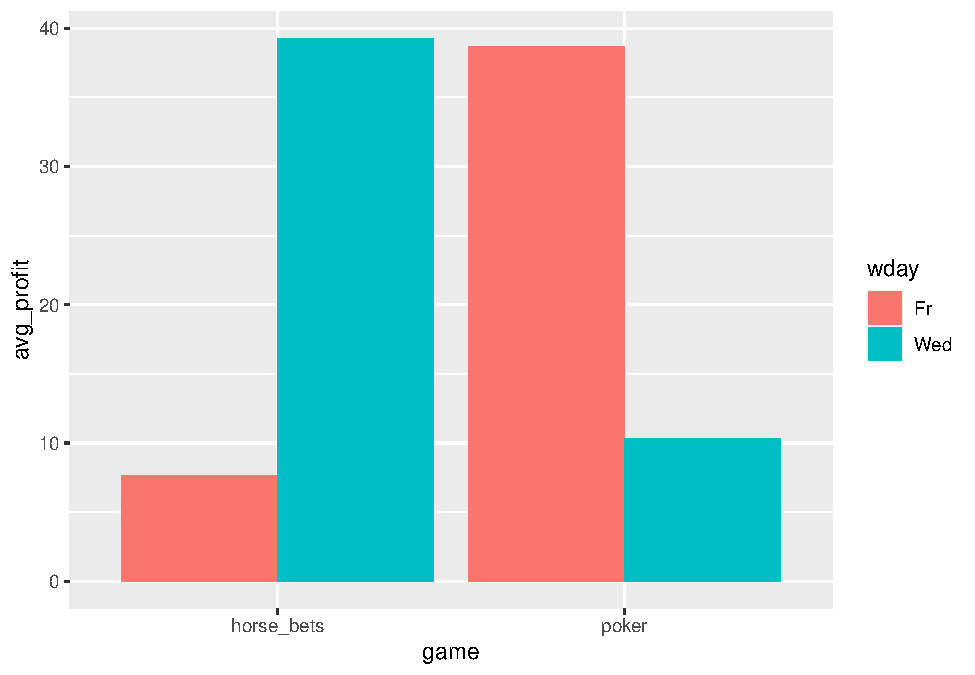
\includegraphics{main_files/figure-latex/unnamed-chunk-92-1.pdf}

\hypertarget{functions-in-this-section}{%
\section{Functions in this section}\label{functions-in-this-section}}

\texttt{data.frame(a\ =\ x,\ b\ =\ y,\ ...)}

Create a data frame from several vectors. The vectors can be different types.

\begin{itemize}
\tightlist
\item
  \texttt{x} A vector with \(n\) elements.
\item
  \texttt{y} Another vector with \(n\) elements.
\item
  \texttt{...} More vectors can be provided.
\end{itemize}

\texttt{View(x)}

Display a data frame, or another structure.

\texttt{head(df,\ n=6)}

Show the first \(n\) rows in the data frame df.

\begin{itemize}
\tightlist
\item
  \texttt{df} Data frame from which to display the first \(n\) rows.
\item
  \texttt{n} The number of rows to display. The default value for \(n\) is 6.
\end{itemize}

\texttt{sum(x)}

Compute the sum of a vector.

\texttt{length(x)}

Return the length of a vector.

\texttt{mean(x)}

Compute the mean of a vector.

\texttt{rep(x,\ n)}

Repeat the contents of a vector \(n\) times

\begin{itemize}
\tightlist
\item
  \texttt{x} The vector to be repeated.
\item
  \texttt{n} How many times to repeat the vector x.
\end{itemize}

\texttt{seq(from,\ to,\ by)}

Create a sequence of integers from \texttt{from} to \texttt{to} in steps of \texttt{by}.

\begin{itemize}
\tightlist
\item
  \texttt{from} The integer to start from.
\item
  \texttt{to} The integer to stop after.
\item
  \texttt{by} Size of steps to take. (If \texttt{from} \(>\) \texttt{to}, \texttt{by} needs to be negative.)
\end{itemize}

\texttt{rbind(df1,\ df2)}

Append df1 to df2 and return the resulting data frame. Both data frames need to have the same number of columns with the same names.

\begin{itemize}
\tightlist
\item
  \texttt{df1} First data frame.
\item
  \texttt{df2} Second data frame.
\end{itemize}

\hypertarget{working-with-data}{%
\chapter{Working with Data}\label{working-with-data}}

In this section, we learn how to work with data in a \textbf{dataframe}. A dataframe is a two-dimensional array consisting of \emph{rows} and \emph{columns}. You can simply think of it as a spreadsheet (e.g.~MS Excel, Google Sheets, etc.).

\hypertarget{basic-dataframes}{%
\section{Basic dataframes}\label{basic-dataframes}}

R has some prebuilt functions to build dataframes. Let us see a simple example. Consider the following three vectors.

\begin{Shaded}
\begin{Highlighting}[]
\NormalTok{name }\OtherTok{\textless{}{-}} \FunctionTok{c}\NormalTok{(}\StringTok{"Sam"}\NormalTok{, }\StringTok{"Paulina"}\NormalTok{, }\StringTok{"Cenk"}\NormalTok{)}
\NormalTok{age }\OtherTok{\textless{}{-}} \FunctionTok{c}\NormalTok{(}\DecValTok{23}\NormalTok{, }\DecValTok{34}\NormalTok{, }\DecValTok{19}\NormalTok{)}
\NormalTok{height }\OtherTok{\textless{}{-}} \FunctionTok{c}\NormalTok{(}\DecValTok{179}\NormalTok{, }\DecValTok{167}\NormalTok{, }\DecValTok{173}\NormalTok{)}
\end{Highlighting}
\end{Shaded}

Let us turn the data stored in different vectors into a single dataframe so that we can visualize the data better.

\begin{Shaded}
\begin{Highlighting}[]
\CommentTok{\#Let us first create the dataframe and assign it to the variable my\_df}
\NormalTok{my\_df }\OtherTok{\textless{}{-}} \FunctionTok{data.frame}\NormalTok{(name,age,height)}

\CommentTok{\#Let\textquotesingle{}s print the dataframe now}
\NormalTok{my\_df}
\end{Highlighting}
\end{Shaded}

\begin{Shaded}
\begin{Highlighting}[]
\NormalTok{\#\#      name age height}
\NormalTok{\#\# 1     Sam  23    179}
\NormalTok{\#\# 2 Paulina  34    167}
\NormalTok{\#\# 3    Cenk  19    173}
\end{Highlighting}
\end{Shaded}

We can select a particular row, column, or cell on a dataframe by using indices. For this we can use the slicing method \texttt{my\_dataframe{[}row,column{]}}.

\begin{Shaded}
\begin{Highlighting}[]
\CommentTok{\#Let us select the entire first row }
\NormalTok{my\_df[}\DecValTok{1}\NormalTok{,]}
\end{Highlighting}
\end{Shaded}

\begin{Shaded}
\begin{Highlighting}[]
\NormalTok{\#\#   name age height}
\NormalTok{\#\# 1  Sam  23    179}
\end{Highlighting}
\end{Shaded}

\begin{Shaded}
\begin{Highlighting}[]
\CommentTok{\#Now, let us select the first column }
\NormalTok{my\_df[,}\DecValTok{1}\NormalTok{]}
\end{Highlighting}
\end{Shaded}

\begin{Shaded}
\begin{Highlighting}[]
\NormalTok{\#\# [1] "Sam"     "Paulina" "Cenk"}
\end{Highlighting}
\end{Shaded}

\begin{Shaded}
\begin{Highlighting}[]
\CommentTok{\#Now, let us find Paulina\textquotesingle{}s height. For this, we need to get the 2nd row and 3rd column.}
\NormalTok{my\_df[}\DecValTok{2}\NormalTok{,}\DecValTok{3}\NormalTok{]}
\end{Highlighting}
\end{Shaded}

\begin{Shaded}
\begin{Highlighting}[]
\NormalTok{\#\# [1] 167}
\end{Highlighting}
\end{Shaded}

\begin{Shaded}
\begin{Highlighting}[]
\CommentTok{\#Now, let us find Paulina\textquotesingle{}s age and height. For this, we need to get the 2nd row and 2nd and 3rd columns.}
\NormalTok{my\_df[}\DecValTok{2}\NormalTok{,}\DecValTok{2}\SpecialCharTok{:}\DecValTok{3}\NormalTok{]}
\end{Highlighting}
\end{Shaded}

\begin{Shaded}
\begin{Highlighting}[]
\NormalTok{\#\#   age height}
\NormalTok{\#\# 2  34    167}
\end{Highlighting}
\end{Shaded}

\begin{Shaded}
\begin{Highlighting}[]
\CommentTok{\#Finally, let us get Sam and Paulina\textquotesingle{}s ages.}
\NormalTok{my\_df[}\DecValTok{1}\SpecialCharTok{:}\DecValTok{2}\NormalTok{,}\DecValTok{2}\NormalTok{]}
\end{Highlighting}
\end{Shaded}

\begin{Shaded}
\begin{Highlighting}[]
\NormalTok{\#\# [1] 23 34}
\end{Highlighting}
\end{Shaded}

You can also use the column name to select an entire column. Just add the dollar sign \texttt{\$} after the df and then the column mane.

\begin{Shaded}
\begin{Highlighting}[]
\NormalTok{my\_df}\SpecialCharTok{$}\NormalTok{age}
\end{Highlighting}
\end{Shaded}

\begin{Shaded}
\begin{Highlighting}[]
\NormalTok{\#\# [1] 23 34 19}
\end{Highlighting}
\end{Shaded}

\hypertarget{tibbles}{%
\section{Tibbles}\label{tibbles}}

The standard dataframes in R are good but not great. Often, we will deal with a lot of data we may not now which index to use to find the value we want. So, we need to be able to have some better ways to access data on our dataframes. We also want to be able to add new data or change some of the existing data easily. For this, we will use various packages in \textbf{tidyverse} for better dataframe management.

Let us first load the tidyverse library, which will load the necessary packages for the functionality described in the following sections.

\begin{Shaded}
\begin{Highlighting}[]
\FunctionTok{library}\NormalTok{(tidyverse)}
\end{Highlighting}
\end{Shaded}

Next, let us introduce tibbles. A \textbf{tibble} is a dataframe with some improved properties. We can turn a regular dataframe into a tibble by calling the \texttt{as\_tibble()} function on our dataframe.

\begin{Shaded}
\begin{Highlighting}[]
\CommentTok{\#Let\textquotesingle{}s turn my\_df into a tibble}
\NormalTok{my\_tibble }\OtherTok{\textless{}{-}} \FunctionTok{as\_tibble}\NormalTok{(my\_df)}

\CommentTok{\#Let\textquotesingle{}s print my\_tibble}
\NormalTok{my\_tibble}
\end{Highlighting}
\end{Shaded}

\begin{Shaded}
\begin{Highlighting}[]
\NormalTok{\#\# \# A tibble: 3 x 3}
\NormalTok{\#\#   name      age height}
\NormalTok{\#\#   \textless{}chr\textgreater{}   \textless{}dbl\textgreater{}  \textless{}dbl\textgreater{}}
\NormalTok{\#\# 1 Sam        23    179}
\NormalTok{\#\# 2 Paulina    34    167}
\NormalTok{\#\# 3 Cenk       19    173}
\end{Highlighting}
\end{Shaded}

As you can see above, the console output tells you that this is a 3x3 tibble meaning that it has 3 rows and 3 columns. It also tells you the type of the data in each column. You can see the data types right under each column name.

\hypertarget{beyond-toy-data}{%
\section{Beyond Toy Data}\label{beyond-toy-data}}

So far we have been working with toy data. In real life projects, you will have a lot more data. The data will usually be stored in some file from which you will have to read into a dataframe. Alternatively, it might be some dataset that from a corpus easily accessible to R. Let us see a few ways in which we can load some realistic datasets into a tibble.

\hypertarget{reading-data-from-a-csv-file}{%
\subsection{Reading data from a csv file}\label{reading-data-from-a-csv-file}}

In this course, we will use some of the data sets from Bodo Winter's book. Go to \href{https://osf.io/34mq9/}{this website} to download the \texttt{materials} folder. Once your data has been downloaded, navigate to the \texttt{materials/data} folder and locate the \texttt{nettle\_1999\_climate.csv} file.

To read in data from a csv to a tibble, we will use the \texttt{read\_csv()} function. All we need to do is to provide the path to the csv file we want to read in. If your csv file is in the same folder as your script, you can simply give its name. Otherwise, you need to provide the relevant directory information as well in your path.

\begin{Shaded}
\begin{Highlighting}[]
\CommentTok{\#Let\textquotesingle{}s read in the data}
\NormalTok{nettle }\OtherTok{\textless{}{-}} \FunctionTok{read\_csv}\NormalTok{(}\StringTok{\textquotesingle{}/Users/umit/Desktop/materials/data/nettle\_1999\_climate.csv\textquotesingle{}}\NormalTok{)}
\end{Highlighting}
\end{Shaded}

\begin{verbatim}
## Rows: 74 Columns: 5
## -- Column specification --------------------------------------------------------
## Delimiter: ","
## chr (1): Country
## dbl (4): Population, Area, MGS, Langs
## 
## i Use `spec()` to retrieve the full column specification for this data.
## i Specify the column types or set `show_col_types = FALSE` to quiet this message.
\end{verbatim}

\begin{Shaded}
\begin{Highlighting}[]
\CommentTok{\#Let\textquotesingle{}s print the head of the data to see what it looks like}
\NormalTok{nettle}
\end{Highlighting}
\end{Shaded}

\begin{Shaded}
\begin{Highlighting}[]
\NormalTok{\#\# \# A tibble: 74 x 5}
\NormalTok{\#\#    Country      Population  Area   MGS Langs}
\NormalTok{\#\#    \textless{}chr\textgreater{}             \textless{}dbl\textgreater{} \textless{}dbl\textgreater{} \textless{}dbl\textgreater{} \textless{}dbl\textgreater{}}
\NormalTok{\#\#  1 Algeria            4.41  6.38  6.6     18}
\NormalTok{\#\#  2 Angola             4.01  6.1   6.22    42}
\NormalTok{\#\#  3 Australia          4.24  6.89  6      234}
\NormalTok{\#\#  4 Bangladesh         5.07  5.16  7.4     37}
\NormalTok{\#\#  5 Benin              3.69  5.05  7.14    52}
\NormalTok{\#\#  6 Bolivia            3.88  6.04  6.92    38}
\NormalTok{\#\#  7 Botswana           3.13  5.76  4.6     27}
\NormalTok{\#\#  8 Brazil             5.19  6.93  9.71   209}
\NormalTok{\#\#  9 Burkina Faso       3.97  5.44  5.17    75}
\NormalTok{\#\# 10 CAR                3.5   5.79  8.08    94}
\NormalTok{\#\# \# ... with 64 more rows}
\end{Highlighting}
\end{Shaded}

If you want to see the last 5 items, use the \texttt{tail()} function.

\begin{Shaded}
\begin{Highlighting}[]
\FunctionTok{tail}\NormalTok{(nettle)}
\end{Highlighting}
\end{Shaded}

\begin{Shaded}
\begin{Highlighting}[]
\NormalTok{\#\# \# A tibble: 6 x 5}
\NormalTok{\#\#   Country   Population  Area   MGS Langs}
\NormalTok{\#\#   \textless{}chr\textgreater{}          \textless{}dbl\textgreater{} \textless{}dbl\textgreater{} \textless{}dbl\textgreater{} \textless{}dbl\textgreater{}}
\NormalTok{\#\# 1 Venezuela       4.31  5.96  7.98    40}
\NormalTok{\#\# 2 Vietnam         4.83  5.52  8.8     88}
\NormalTok{\#\# 3 Yemen           4.09  5.72  0        6}
\NormalTok{\#\# 4 Zaire           4.56  6.37  9.44   219}
\NormalTok{\#\# 5 Zambia          3.94  5.88  5.43    38}
\NormalTok{\#\# 6 Zimbabwe        4     5.59  5.29    18}
\end{Highlighting}
\end{Shaded}

If you want to view the entire dataset, you can use \texttt{View(nettle)}. This will open a new tab in RStudio and show your data as a table.

\hypertarget{reading-data-from-r-data-packages}{%
\subsection{Reading data from R data packages}\label{reading-data-from-r-data-packages}}

R has various data packages you can install and use. Let us install the \texttt{languageR} which has some nice language datasets. Once you install the package and load the library, you can easily use the datasets as tibles. For all the details and available datasets in \texttt{languageR}, you can check the \href{https://cran.r-project.org/web/packages/languageR/languageR.pdf}{languageR documentation} on CRAN.

\begin{Shaded}
\begin{Highlighting}[]
\CommentTok{\#Let\textquotesingle{}s load the library}
\FunctionTok{library}\NormalTok{(languageR)}

\CommentTok{\#We\textquotesingle{}ll use the dativeSimplified dataset, which is documented. Let\textquotesingle{}s see the documentation}
\NormalTok{?dativeSimplified}
\end{Highlighting}
\end{Shaded}

\begin{Shaded}
\begin{Highlighting}[]
\CommentTok{\#let\textquotesingle{}s use the dativeSimplified data from the languageR }
\NormalTok{data }\OtherTok{\textless{}{-}} \FunctionTok{as\_tibble}\NormalTok{(dativeSimplified)}

\CommentTok{\#Let\textquotesingle{}s print the first few lines of the data}
\NormalTok{data}
\end{Highlighting}
\end{Shaded}

\begin{Shaded}
\begin{Highlighting}[]
\NormalTok{\#\# \# A tibble: 903 x 5}
\NormalTok{\#\#    RealizationOfRec Verb  AnimacyOfRec AnimacyOfTheme LengthOfTheme}
\NormalTok{\#\#    \textless{}fct\textgreater{}            \textless{}fct\textgreater{} \textless{}fct\textgreater{}        \textless{}fct\textgreater{}                  \textless{}dbl\textgreater{}}
\NormalTok{\#\#  1 NP               feed  animate      inanimate              2.64 }
\NormalTok{\#\#  2 NP               give  animate      inanimate              1.10 }
\NormalTok{\#\#  3 NP               give  animate      inanimate              2.56 }
\NormalTok{\#\#  4 NP               give  animate      inanimate              1.61 }
\NormalTok{\#\#  5 NP               offer animate      inanimate              1.10 }
\NormalTok{\#\#  6 NP               give  animate      inanimate              1.39 }
\NormalTok{\#\#  7 NP               pay   animate      inanimate              1.39 }
\NormalTok{\#\#  8 NP               bring animate      inanimate              0    }
\NormalTok{\#\#  9 NP               teach animate      inanimate              2.40 }
\NormalTok{\#\# 10 NP               give  animate      inanimate              0.693}
\NormalTok{\#\# \# ... with 893 more rows}
\end{Highlighting}
\end{Shaded}

\textbf{Dative Alternation} is the phenomenon in English where a recipient of a ditransitive verb can occur as an NP or a PP.

\begin{enumerate}
\def\labelenumi{\arabic{enumi}.}
\tightlist
\item
  Alex gave Sam a book.
\item
  Alex gave a book to Sam.
\end{enumerate}

Both of these constructions are grammatical and they mean essentially the same thing. The question is what factors are involved in picking one of the forms over the other. Bresnan et al.~(2007) used this data to determine the relevant factors.
Let us randomly select 10 examples and see what they look like. For that, we can use the folloing code.

\begin{Shaded}
\begin{Highlighting}[]
\CommentTok{\# store all possible row indices in a vector}
\NormalTok{indices\_all }\OtherTok{\textless{}{-}} \DecValTok{1}\SpecialCharTok{:}\FunctionTok{nrow}\NormalTok{(data)}

\CommentTok{\# set the random seed to make the results reproducible}
\FunctionTok{set.seed}\NormalTok{(}\DecValTok{123}\NormalTok{)}

\CommentTok{\# choose 10 such numbers at random without replacement}
\NormalTok{indices\_random }\OtherTok{\textless{}{-}} \FunctionTok{sample}\NormalTok{(indices\_all, }\AttributeTok{size =} \DecValTok{10}\NormalTok{)}

\CommentTok{\# use them to index the data frame to get the corresponding rows}
\NormalTok{data[indices\_random,]}
\end{Highlighting}
\end{Shaded}

\begin{Shaded}
\begin{Highlighting}[]
\NormalTok{\#\# \# A tibble: 10 x 5}
\NormalTok{\#\#    RealizationOfRec Verb  AnimacyOfRec AnimacyOfTheme LengthOfTheme}
\NormalTok{\#\#    \textless{}fct\textgreater{}            \textless{}fct\textgreater{} \textless{}fct\textgreater{}        \textless{}fct\textgreater{}                  \textless{}dbl\textgreater{}}
\NormalTok{\#\#  1 NP               give  inanimate    inanimate              1.79 }
\NormalTok{\#\#  2 NP               grant animate      inanimate              1.10 }
\NormalTok{\#\#  3 NP               grant animate      inanimate              2.40 }
\NormalTok{\#\#  4 NP               give  animate      inanimate              2.56 }
\NormalTok{\#\#  5 NP               tell  animate      inanimate              3.26 }
\NormalTok{\#\#  6 PP               give  animate      inanimate              0    }
\NormalTok{\#\#  7 NP               pay   animate      inanimate              0.693}
\NormalTok{\#\#  8 NP               hand  animate      inanimate              0.693}
\NormalTok{\#\#  9 NP               give  inanimate    inanimate              1.61 }
\NormalTok{\#\# 10 NP               wish  animate      inanimate              1.10}
\end{Highlighting}
\end{Shaded}

\hypertarget{summarizing-data}{%
\section{Summarizing Data}\label{summarizing-data}}

Looking at the summary statistics of your data is always a good first step. Let's take a look at the percentage of NP realizations of the recipient by animacy of the theme.

\begin{Shaded}
\begin{Highlighting}[]
\CommentTok{\# First, let\textquotesingle{}s take a look at the key dependet variable (NP or PP)}

\FunctionTok{unique}\NormalTok{(data}\SpecialCharTok{$}\NormalTok{RealizationOfRec)}
\end{Highlighting}
\end{Shaded}

\begin{Shaded}
\begin{Highlighting}[]
\NormalTok{\#\# [1] NP PP}
\NormalTok{\#\# Levels: NP PP}
\end{Highlighting}
\end{Shaded}

\begin{Shaded}
\begin{Highlighting}[]
\CommentTok{\# now, let\textquotesingle{}s compute the percentages (perc\_NP) and the number of observations in each subset}
\NormalTok{data}\SpecialCharTok{\%\textgreater{}\%} 
  \FunctionTok{group\_by}\NormalTok{(AnimacyOfRec) }\SpecialCharTok{\%\textgreater{}\%} 
  \FunctionTok{summarize}\NormalTok{(}\AttributeTok{perc\_NP =} \FunctionTok{mean}\NormalTok{(RealizationOfRec }\SpecialCharTok{==} \StringTok{"NP"}\NormalTok{), }
                   \AttributeTok{N =} \FunctionTok{n}\NormalTok{()}
\NormalTok{                  )}
\end{Highlighting}
\end{Shaded}

\begin{Shaded}
\begin{Highlighting}[]
\NormalTok{\#\# \# A tibble: 2 x 3}
\NormalTok{\#\#   AnimacyOfRec perc\_NP     N}
\NormalTok{\#\#   \textless{}fct\textgreater{}          \textless{}dbl\textgreater{} \textless{}int\textgreater{}}
\NormalTok{\#\# 1 animate        0.634   822}
\NormalTok{\#\# 2 inanimate      0.420    81}
\end{Highlighting}
\end{Shaded}

\textbf{What do the results say?}

\begin{itemize}
\tightlist
\item
  There are a total of 822 instances of animate recipients.
\item
  63\% of the animate recipients are NPs.
\end{itemize}

\hypertarget{working-with-dplyr}{%
\section{Working with dplyr}\label{working-with-dplyr}}

One of the packages in the \texttt{tidyverse} is \texttt{dplyr}. We use it to do various manipulations on the data frames. Check out the \href{https://nyu-cdsc.github.io/learningr/assets/data-transformation.pdf}{dplyr cheatsheet} for further details.

The \texttt{arrange} function will arrange your data in an ascending order.

\begin{Shaded}
\begin{Highlighting}[]
\FunctionTok{arrange}\NormalTok{(data)}
\end{Highlighting}
\end{Shaded}

\begin{Shaded}
\begin{Highlighting}[]
\NormalTok{\#\# \# A tibble: 903 x 5}
\NormalTok{\#\#    RealizationOfRec Verb  AnimacyOfRec AnimacyOfTheme LengthOfTheme}
\NormalTok{\#\#    \textless{}fct\textgreater{}            \textless{}fct\textgreater{} \textless{}fct\textgreater{}        \textless{}fct\textgreater{}                  \textless{}dbl\textgreater{}}
\NormalTok{\#\#  1 NP               feed  animate      inanimate              2.64 }
\NormalTok{\#\#  2 NP               give  animate      inanimate              1.10 }
\NormalTok{\#\#  3 NP               give  animate      inanimate              2.56 }
\NormalTok{\#\#  4 NP               give  animate      inanimate              1.61 }
\NormalTok{\#\#  5 NP               offer animate      inanimate              1.10 }
\NormalTok{\#\#  6 NP               give  animate      inanimate              1.39 }
\NormalTok{\#\#  7 NP               pay   animate      inanimate              1.39 }
\NormalTok{\#\#  8 NP               bring animate      inanimate              0    }
\NormalTok{\#\#  9 NP               teach animate      inanimate              2.40 }
\NormalTok{\#\# 10 NP               give  animate      inanimate              0.693}
\NormalTok{\#\# \# ... with 893 more rows}
\end{Highlighting}
\end{Shaded}

You can arrange the data based on a particular column. In that case, you need to provide the column name.

\begin{Shaded}
\begin{Highlighting}[]
\FunctionTok{arrange}\NormalTok{(data,LengthOfTheme)}
\end{Highlighting}
\end{Shaded}

\begin{Shaded}
\begin{Highlighting}[]
\NormalTok{\#\# \# A tibble: 903 x 5}
\NormalTok{\#\#    RealizationOfRec Verb   AnimacyOfRec AnimacyOfTheme LengthOfTheme}
\NormalTok{\#\#    \textless{}fct\textgreater{}            \textless{}fct\textgreater{}  \textless{}fct\textgreater{}        \textless{}fct\textgreater{}                  \textless{}dbl\textgreater{}}
\NormalTok{\#\#  1 NP               bring  animate      inanimate                  0}
\NormalTok{\#\#  2 NP               send   animate      inanimate                  0}
\NormalTok{\#\#  3 NP               bet    animate      inanimate                  0}
\NormalTok{\#\#  4 NP               tell   animate      inanimate                  0}
\NormalTok{\#\#  5 NP               tell   animate      inanimate                  0}
\NormalTok{\#\#  6 NP               give   inanimate    inanimate                  0}
\NormalTok{\#\#  7 NP               give   animate      inanimate                  0}
\NormalTok{\#\#  8 NP               charge animate      inanimate                  0}
\NormalTok{\#\#  9 NP               give   animate      inanimate                  0}
\NormalTok{\#\# 10 NP               pay    animate      inanimate                  0}
\NormalTok{\#\# \# ... with 893 more rows}
\end{Highlighting}
\end{Shaded}

\begin{Shaded}
\begin{Highlighting}[]
\FunctionTok{arrange}\NormalTok{(data[}\DecValTok{1}\SpecialCharTok{:}\DecValTok{10}\NormalTok{,], LengthOfTheme)}
\end{Highlighting}
\end{Shaded}

\begin{Shaded}
\begin{Highlighting}[]
\NormalTok{\#\# \# A tibble: 10 x 5}
\NormalTok{\#\#    RealizationOfRec Verb  AnimacyOfRec AnimacyOfTheme LengthOfTheme}
\NormalTok{\#\#    \textless{}fct\textgreater{}            \textless{}fct\textgreater{} \textless{}fct\textgreater{}        \textless{}fct\textgreater{}                  \textless{}dbl\textgreater{}}
\NormalTok{\#\#  1 NP               bring animate      inanimate              0    }
\NormalTok{\#\#  2 NP               give  animate      inanimate              0.693}
\NormalTok{\#\#  3 NP               give  animate      inanimate              1.10 }
\NormalTok{\#\#  4 NP               offer animate      inanimate              1.10 }
\NormalTok{\#\#  5 NP               give  animate      inanimate              1.39 }
\NormalTok{\#\#  6 NP               pay   animate      inanimate              1.39 }
\NormalTok{\#\#  7 NP               give  animate      inanimate              1.61 }
\NormalTok{\#\#  8 NP               teach animate      inanimate              2.40 }
\NormalTok{\#\#  9 NP               give  animate      inanimate              2.56 }
\NormalTok{\#\# 10 NP               feed  animate      inanimate              2.64}
\end{Highlighting}
\end{Shaded}

If you want to arrange things in a descending order, then you need to put the \texttt{desc()} function around the relevant column.

\begin{Shaded}
\begin{Highlighting}[]
\FunctionTok{arrange}\NormalTok{(data, }\FunctionTok{desc}\NormalTok{(LengthOfTheme))}
\end{Highlighting}
\end{Shaded}

\begin{Shaded}
\begin{Highlighting}[]
\NormalTok{\#\# \# A tibble: 903 x 5}
\NormalTok{\#\#    RealizationOfRec Verb  AnimacyOfRec AnimacyOfTheme LengthOfTheme}
\NormalTok{\#\#    \textless{}fct\textgreater{}            \textless{}fct\textgreater{} \textless{}fct\textgreater{}        \textless{}fct\textgreater{}                  \textless{}dbl\textgreater{}}
\NormalTok{\#\#  1 NP               give  inanimate    inanimate               3.64}
\NormalTok{\#\#  2 NP               send  animate      inanimate               3.56}
\NormalTok{\#\#  3 NP               give  animate      inanimate               3.53}
\NormalTok{\#\#  4 NP               pay   animate      inanimate               3.50}
\NormalTok{\#\#  5 NP               give  animate      inanimate               3.50}
\NormalTok{\#\#  6 NP               give  animate      inanimate               3.47}
\NormalTok{\#\#  7 NP               give  animate      inanimate               3.47}
\NormalTok{\#\#  8 NP               give  animate      inanimate               3.40}
\NormalTok{\#\#  9 NP               send  animate      inanimate               3.40}
\NormalTok{\#\# 10 NP               give  animate      inanimate               3.37}
\NormalTok{\#\# \# ... with 893 more rows}
\end{Highlighting}
\end{Shaded}

Another useful function is the \texttt{select()} function which allows you to create new dataframes using only columns you want.

\begin{Shaded}
\begin{Highlighting}[]
\CommentTok{\#Create the new dataframe using select}
\NormalTok{df }\OtherTok{\textless{}{-}} \FunctionTok{select}\NormalTok{(data, Verb, LengthOfTheme)}

\CommentTok{\#print the head}
\NormalTok{df}
\end{Highlighting}
\end{Shaded}

\begin{Shaded}
\begin{Highlighting}[]
\NormalTok{\#\# \# A tibble: 903 x 2}
\NormalTok{\#\#    Verb  LengthOfTheme}
\NormalTok{\#\#    \textless{}fct\textgreater{}         \textless{}dbl\textgreater{}}
\NormalTok{\#\#  1 feed          2.64 }
\NormalTok{\#\#  2 give          1.10 }
\NormalTok{\#\#  3 give          2.56 }
\NormalTok{\#\#  4 give          1.61 }
\NormalTok{\#\#  5 offer         1.10 }
\NormalTok{\#\#  6 give          1.39 }
\NormalTok{\#\#  7 pay           1.39 }
\NormalTok{\#\#  8 bring         0    }
\NormalTok{\#\#  9 teach         2.40 }
\NormalTok{\#\# 10 give          0.693}
\NormalTok{\#\# \# ... with 893 more rows}
\end{Highlighting}
\end{Shaded}

Another useful function is \texttt{sample\_n()} which randomly samples some number of datapoints.

\begin{Shaded}
\begin{Highlighting}[]
\FunctionTok{sample\_n}\NormalTok{(data, }\DecValTok{5}\NormalTok{)}
\end{Highlighting}
\end{Shaded}

\begin{Shaded}
\begin{Highlighting}[]
\NormalTok{\#\# \# A tibble: 5 x 5}
\NormalTok{\#\#   RealizationOfRec Verb  AnimacyOfRec AnimacyOfTheme LengthOfTheme}
\NormalTok{\#\#   \textless{}fct\textgreater{}            \textless{}fct\textgreater{} \textless{}fct\textgreater{}        \textless{}fct\textgreater{}                  \textless{}dbl\textgreater{}}
\NormalTok{\#\# 1 NP               give  animate      inanimate              0.693}
\NormalTok{\#\# 2 NP               sell  animate      inanimate              0    }
\NormalTok{\#\# 3 PP               give  animate      inanimate              1.61 }
\NormalTok{\#\# 4 PP               pay   animate      inanimate              1.39 }
\NormalTok{\#\# 5 PP               offer inanimate    inanimate              1.95}
\end{Highlighting}
\end{Shaded}

Two other useful functions are \texttt{group\_by()} and \texttt{ungroup()}.

\begin{Shaded}
\begin{Highlighting}[]
\CommentTok{\#Let\textquotesingle{}s group a small portion of the data by the realization of recipient}
\FunctionTok{group\_by}\NormalTok{(data[}\DecValTok{1}\SpecialCharTok{:}\DecValTok{5}\NormalTok{], RealizationOfRec)}
\end{Highlighting}
\end{Shaded}

\begin{Shaded}
\begin{Highlighting}[]
\NormalTok{\#\# \# A tibble: 903 x 5}
\NormalTok{\#\# \# Groups:   RealizationOfRec [2]}
\NormalTok{\#\#    RealizationOfRec Verb  AnimacyOfRec AnimacyOfTheme LengthOfTheme}
\NormalTok{\#\#    \textless{}fct\textgreater{}            \textless{}fct\textgreater{} \textless{}fct\textgreater{}        \textless{}fct\textgreater{}                  \textless{}dbl\textgreater{}}
\NormalTok{\#\#  1 NP               feed  animate      inanimate              2.64 }
\NormalTok{\#\#  2 NP               give  animate      inanimate              1.10 }
\NormalTok{\#\#  3 NP               give  animate      inanimate              2.56 }
\NormalTok{\#\#  4 NP               give  animate      inanimate              1.61 }
\NormalTok{\#\#  5 NP               offer animate      inanimate              1.10 }
\NormalTok{\#\#  6 NP               give  animate      inanimate              1.39 }
\NormalTok{\#\#  7 NP               pay   animate      inanimate              1.39 }
\NormalTok{\#\#  8 NP               bring animate      inanimate              0    }
\NormalTok{\#\#  9 NP               teach animate      inanimate              2.40 }
\NormalTok{\#\# 10 NP               give  animate      inanimate              0.693}
\NormalTok{\#\# \# ... with 893 more rows}
\end{Highlighting}
\end{Shaded}

Now let us group the data by verbs.

\begin{Shaded}
\begin{Highlighting}[]
\NormalTok{data\_grouped\_by\_verb }\OtherTok{\textless{}{-}} \FunctionTok{group\_by}\NormalTok{(data,Verb)}
\end{Highlighting}
\end{Shaded}

An important but complex function is the \texttt{summarize()} function.

\begin{enumerate}
\def\labelenumi{\arabic{enumi}.}
\tightlist
\item
  It divides a grouped data frame into subsets, with each subset corresponding to one value of the grouping variable (or a combination of values for several grouping variables).
\item
  It computes one or several values we specify on each such subset.
\item
  It creates a new data frame and puts everything together. The first column of this new data frame consists of levels of our grouping variable. In the following columns, the summarize() function prints the results of the computations we have specified.
\end{enumerate}

Try to guess the result of the following code. What will you see as an output? What will be the name of the columns?

\begin{Shaded}
\begin{Highlighting}[]
\CommentTok{\# summarize several variables}
\FunctionTok{summarize}\NormalTok{(data\_grouped\_by\_verb, }
          \AttributeTok{prop\_animate\_rec =} \FunctionTok{mean}\NormalTok{( AnimacyOfRec }\SpecialCharTok{==} \StringTok{"animate"}\NormalTok{ ),}
          \AttributeTok{prop\_animate\_theme =} \FunctionTok{mean}\NormalTok{( AnimacyOfTheme }\SpecialCharTok{==} \StringTok{"animate"}\NormalTok{ ),}
          \AttributeTok{N =} \FunctionTok{n}\NormalTok{()}
\NormalTok{          )}
\end{Highlighting}
\end{Shaded}

\begin{Shaded}
\begin{Highlighting}[]
\NormalTok{\#\# \# A tibble: 65 x 4}
\NormalTok{\#\#    Verb     prop\_animate\_rec prop\_animate\_theme     N}
\NormalTok{\#\#    \textless{}fct\textgreater{}               \textless{}dbl\textgreater{}              \textless{}dbl\textgreater{} \textless{}int\textgreater{}}
\NormalTok{\#\#  1 accord              1                      0     1}
\NormalTok{\#\#  2 allocate            0                      0     3}
\NormalTok{\#\#  3 allow               0.833                  0     6}
\NormalTok{\#\#  4 assess              1                      0     1}
\NormalTok{\#\#  5 assure              1                      0     2}
\NormalTok{\#\#  6 award               0.944                  0    18}
\NormalTok{\#\#  7 bequeath            1                      0     1}
\NormalTok{\#\#  8 bet                 1                      0     1}
\NormalTok{\#\#  9 bring               0.818                  0    11}
\NormalTok{\#\# 10 carry               1                      0     1}
\NormalTok{\#\# \# ... with 55 more rows}
\end{Highlighting}
\end{Shaded}

Try to interpret the output of the following code.

\begin{Shaded}
\begin{Highlighting}[]
\CommentTok{\# compute the averages}
\FunctionTok{summarize}\NormalTok{(data\_grouped\_by\_verb, }
          \AttributeTok{prop\_anim =} \FunctionTok{mean}\NormalTok{(AnimacyOfRec }\SpecialCharTok{==} \StringTok{"animate"}\NormalTok{),}
          \AttributeTok{prop\_inanim =} \DecValTok{1}\SpecialCharTok{{-}}\NormalTok{prop\_anim,}
          \AttributeTok{prop\_v\_recip\_anim =} \FunctionTok{ifelse}\NormalTok{(prop\_anim }\SpecialCharTok{\textgreater{}} \FloatTok{0.5}\NormalTok{, }\StringTok{"high"}\NormalTok{, }\StringTok{"low"}\NormalTok{)}
\NormalTok{          )}
\end{Highlighting}
\end{Shaded}

\begin{Shaded}
\begin{Highlighting}[]
\NormalTok{\#\# \# A tibble: 65 x 4}
\NormalTok{\#\#    Verb     prop\_anim prop\_inanim prop\_v\_recip\_anim}
\NormalTok{\#\#    \textless{}fct\textgreater{}        \textless{}dbl\textgreater{}       \textless{}dbl\textgreater{} \textless{}chr\textgreater{}            }
\NormalTok{\#\#  1 accord       1          0      high             }
\NormalTok{\#\#  2 allocate     0          1      low              }
\NormalTok{\#\#  3 allow        0.833      0.167  high             }
\NormalTok{\#\#  4 assess       1          0      high             }
\NormalTok{\#\#  5 assure       1          0      high             }
\NormalTok{\#\#  6 award        0.944      0.0556 high             }
\NormalTok{\#\#  7 bequeath     1          0      high             }
\NormalTok{\#\#  8 bet          1          0      high             }
\NormalTok{\#\#  9 bring        0.818      0.182  high             }
\NormalTok{\#\# 10 carry        1          0      high             }
\NormalTok{\#\# \# ... with 55 more rows}
\end{Highlighting}
\end{Shaded}

The last line uses the function ifelse(condition, value1, value2), which, for each element of the condition vector returns the corresponding element of the value1 vector if the condition is true at that element, or an element of vector2 otherwise.

mutate() proceeds similarly to summarize() in dividing a grouped dataset into subsets, but instead of computing one or several values for each subset, it creates or modifies a column.

The main difference between mutate() and summarize() is the output. While mutate() modifies the original and returns a modified version of it, summarize() creates a brand new data frame with one row for every combination of the the grouping variable values.

A very simple application of mutate() is to simply create a new column. In this case, we don't even need to group.

\begin{Shaded}
\begin{Highlighting}[]
\CommentTok{\# these two lines performs exactly the same action, }
\CommentTok{\# except the latter stores the result in df }
\NormalTok{data}\SpecialCharTok{$}\NormalTok{is\_realization\_NP }\OtherTok{\textless{}{-}}\NormalTok{ (data}\SpecialCharTok{$}\NormalTok{RealizationOfRec }\SpecialCharTok{==} \StringTok{"NP"}\NormalTok{ ) }
\NormalTok{df }\OtherTok{\textless{}{-}} \FunctionTok{mutate}\NormalTok{(data, }\AttributeTok{is\_realization\_NP =}\NormalTok{ (RealizationOfRec }\SpecialCharTok{==} \StringTok{"NP"}\NormalTok{) )}

\FunctionTok{head}\NormalTok{(df, }\DecValTok{2}\NormalTok{)}
\end{Highlighting}
\end{Shaded}

\begin{Shaded}
\begin{Highlighting}[]
\NormalTok{\#\# \# A tibble: 2 x 6}
\NormalTok{\#\#   RealizationOfRec Verb  AnimacyOfRec AnimacyOfTheme LengthOfTheme is\_realizat\textasciitilde{}1}
\NormalTok{\#\#   \textless{}fct\textgreater{}            \textless{}fct\textgreater{} \textless{}fct\textgreater{}        \textless{}fct\textgreater{}                  \textless{}dbl\textgreater{} \textless{}lgl\textgreater{}        }
\NormalTok{\#\# 1 NP               feed  animate      inanimate               2.64 TRUE         }
\NormalTok{\#\# 2 NP               give  animate      inanimate               1.10 TRUE         }
\NormalTok{\#\# \# ... with abbreviated variable name 1: is\_realization\_NP}
\end{Highlighting}
\end{Shaded}

One final useful function is the \texttt{filter()} function. It allows you to find rows by particular values of a column.

\begin{Shaded}
\begin{Highlighting}[]
\FunctionTok{filter}\NormalTok{(data, is\_realization\_NP }\SpecialCharTok{==} \ConstantTok{FALSE}\NormalTok{)}
\end{Highlighting}
\end{Shaded}

\begin{Shaded}
\begin{Highlighting}[]
\NormalTok{\#\# \# A tibble: 348 x 6}
\NormalTok{\#\#    RealizationOfRec Verb  AnimacyOfRec AnimacyOfTheme LengthOfTheme is\_realiza\textasciitilde{}1}
\NormalTok{\#\#    \textless{}fct\textgreater{}            \textless{}fct\textgreater{} \textless{}fct\textgreater{}        \textless{}fct\textgreater{}                  \textless{}dbl\textgreater{} \textless{}lgl\textgreater{}       }
\NormalTok{\#\#  1 PP               give  animate      inanimate              0     FALSE       }
\NormalTok{\#\#  2 PP               give  inanimate    inanimate              1.79  FALSE       }
\NormalTok{\#\#  3 PP               give  animate      inanimate              1.39  FALSE       }
\NormalTok{\#\#  4 PP               give  animate      inanimate              1.39  FALSE       }
\NormalTok{\#\#  5 PP               sell  animate      inanimate              1.79  FALSE       }
\NormalTok{\#\#  6 PP               give  inanimate    inanimate              0.693 FALSE       }
\NormalTok{\#\#  7 PP               give  inanimate    inanimate              0.693 FALSE       }
\NormalTok{\#\#  8 PP               give  animate      inanimate              1.39  FALSE       }
\NormalTok{\#\#  9 PP               send  animate      inanimate              2.56  FALSE       }
\NormalTok{\#\# 10 PP               offer animate      inanimate              1.95  FALSE       }
\NormalTok{\#\# \# ... with 338 more rows, and abbreviated variable name 1: is\_realization\_NP}
\end{Highlighting}
\end{Shaded}

\begin{Shaded}
\begin{Highlighting}[]
\FunctionTok{filter}\NormalTok{(data, LengthOfTheme }\SpecialCharTok{\textgreater{}} \FloatTok{3.5}\NormalTok{)}
\end{Highlighting}
\end{Shaded}

\begin{Shaded}
\begin{Highlighting}[]
\NormalTok{\#\# \# A tibble: 3 x 6}
\NormalTok{\#\#   RealizationOfRec Verb  AnimacyOfRec AnimacyOfTheme LengthOfTheme is\_realizat\textasciitilde{}1}
\NormalTok{\#\#   \textless{}fct\textgreater{}            \textless{}fct\textgreater{} \textless{}fct\textgreater{}        \textless{}fct\textgreater{}                  \textless{}dbl\textgreater{} \textless{}lgl\textgreater{}        }
\NormalTok{\#\# 1 NP               send  animate      inanimate               3.56 TRUE         }
\NormalTok{\#\# 2 NP               give  animate      inanimate               3.53 TRUE         }
\NormalTok{\#\# 3 NP               give  inanimate    inanimate               3.64 TRUE         }
\NormalTok{\#\# \# ... with abbreviated variable name 1: is\_realization\_NP}
\end{Highlighting}
\end{Shaded}

\hypertarget{pipes}{%
\section{Pipes}\label{pipes}}

\hypertarget{the-problem}{%
\subsection{The problem}\label{the-problem}}

\begin{itemize}
\tightlist
\item
  The code below is really hard to read, even harder to maintain, and \texttt{dativeSimplified\_grouped\_by\_AnimacyOfRec\_and\_AnimacyOfTheme} is a terribly long variable name.
\end{itemize}

\begin{Shaded}
\begin{Highlighting}[]
\NormalTok{dativeSimplified\_grouped\_by\_AnimacyOfRec\_and\_AnimacyOfTheme }\OtherTok{\textless{}{-}}
      \FunctionTok{group\_by}\NormalTok{(dativeSimplified, AnimacyOfRec, AnimacyOfTheme)}
\NormalTok{df }\OtherTok{\textless{}{-}} \FunctionTok{summarize}\NormalTok{(dativeSimplified\_grouped\_by\_AnimacyOfRec\_and\_AnimacyOfTheme, }
                  \AttributeTok{perc\_NP =} \FunctionTok{mean}\NormalTok{(RealizationOfRec }\SpecialCharTok{==} \StringTok{"NP"}\NormalTok{) )}
\end{Highlighting}
\end{Shaded}

\begin{verbatim}
## `summarise()` has grouped output by 'AnimacyOfRec'. You can override using the
## `.groups` argument.
\end{verbatim}

\begin{Shaded}
\begin{Highlighting}[]
\NormalTok{df}
\end{Highlighting}
\end{Shaded}

\begin{Shaded}
\begin{Highlighting}[]
\NormalTok{\#\# \# A tibble: 4 x 3}
\NormalTok{\#\# \# Groups:   AnimacyOfRec [2]}
\NormalTok{\#\#   AnimacyOfRec AnimacyOfTheme perc\_NP}
\NormalTok{\#\#   \textless{}fct\textgreater{}        \textless{}fct\textgreater{}            \textless{}dbl\textgreater{}}
\NormalTok{\#\# 1 animate      animate          0.8  }
\NormalTok{\#\# 2 animate      inanimate        0.633}
\NormalTok{\#\# 3 inanimate    animate          1    }
\NormalTok{\#\# 4 inanimate    inanimate        0.412}
\end{Highlighting}
\end{Shaded}

\begin{itemize}
\tightlist
\item
  This alternative is also quite bad. To read this code, you need to know which bracket matches which other bracket.
\end{itemize}

\begin{Shaded}
\begin{Highlighting}[]
\NormalTok{df }\OtherTok{\textless{}{-}} \FunctionTok{summarize}\NormalTok{(}\FunctionTok{group\_by}\NormalTok{(dativeSimplified, AnimacyOfRec, AnimacyOfTheme), }
                  \AttributeTok{perc\_NP =} \FunctionTok{mean}\NormalTok{(RealizationOfRec }\SpecialCharTok{==} \StringTok{"NP"}\NormalTok{) )}
\end{Highlighting}
\end{Shaded}

\begin{verbatim}
## `summarise()` has grouped output by 'AnimacyOfRec'. You can override using the
## `.groups` argument.
\end{verbatim}

\begin{Shaded}
\begin{Highlighting}[]
\NormalTok{df}
\end{Highlighting}
\end{Shaded}

\begin{Shaded}
\begin{Highlighting}[]
\NormalTok{\#\# \# A tibble: 4 x 3}
\NormalTok{\#\# \# Groups:   AnimacyOfRec [2]}
\NormalTok{\#\#   AnimacyOfRec AnimacyOfTheme perc\_NP}
\NormalTok{\#\#   \textless{}fct\textgreater{}        \textless{}fct\textgreater{}            \textless{}dbl\textgreater{}}
\NormalTok{\#\# 1 animate      animate          0.8  }
\NormalTok{\#\# 2 animate      inanimate        0.633}
\NormalTok{\#\# 3 inanimate    animate          1    }
\NormalTok{\#\# 4 inanimate    inanimate        0.412}
\end{Highlighting}
\end{Shaded}

\begin{itemize}
\tightlist
\item
  One nested function call may be OK. But try to read this.
\end{itemize}

\begin{Shaded}
\begin{Highlighting}[]
\NormalTok{df }\OtherTok{\textless{}{-}}\NormalTok{ dplyr}\SpecialCharTok{::}\FunctionTok{summarize}\NormalTok{(}\FunctionTok{group\_by}\NormalTok{(}\FunctionTok{mutate}\NormalTok{(dativeSimplified, }\AttributeTok{long\_theme =} \FunctionTok{ifelse}\NormalTok{(LengthOfTheme }\SpecialCharTok{\textgreater{}} \FloatTok{1.6}\NormalTok{, }\StringTok{"long"}\NormalTok{, }\StringTok{"short"}\NormalTok{) ), long\_theme),}
              \AttributeTok{perc\_NP =} \FunctionTok{mean}\NormalTok{(RealizationOfRec }\SpecialCharTok{==} \StringTok{"NP"}\NormalTok{)}
\NormalTok{              )}
\end{Highlighting}
\end{Shaded}

\begin{itemize}
\tightlist
\item
  Or consider this expression (\texttt{sqrt} is the square root.)
\end{itemize}

\begin{Shaded}
\begin{Highlighting}[]
\FunctionTok{sqrt}\NormalTok{(}\FunctionTok{divide\_by}\NormalTok{(}\FunctionTok{sum}\NormalTok{(}\FunctionTok{divide\_by}\NormalTok{(}\DecValTok{2}\NormalTok{,}\DecValTok{3}\NormalTok{), }\FunctionTok{multiply\_by}\NormalTok{(}\DecValTok{2}\NormalTok{,}\DecValTok{3}\NormalTok{)), }\FunctionTok{sum}\NormalTok{(}\DecValTok{3}\NormalTok{,}\DecValTok{4}\NormalTok{)))}
\end{Highlighting}
\end{Shaded}

\begin{Shaded}
\begin{Highlighting}[]
\NormalTok{\#\# [1] 0.9759001}
\end{Highlighting}
\end{Shaded}

\begin{itemize}
\tightlist
\item
  Luckily, there a better way to write this expression.
\end{itemize}

\hypertarget{pipes-1}{%
\subsection{Pipes}\label{pipes-1}}

\begin{itemize}
\tightlist
\item
  The problem is that we have too many levels of embedding.
\item
  In natural language we avoid multiple embeddings of that sort by making shorter sentences, and using anaphors to refer to previous discourse.
\item
  The packages \textbf{dplyr} and \textbf{magrittr} provide a limited version of such functionality, and we'll need to use \textbf{pipe} operators (\texttt{\%\textgreater{}\%} and \texttt{\%\textless{}\textgreater{}\%}) to link expressions with an `anaphoric dependency'.
\item
  Whenever you see \texttt{\%\textgreater{}\%}, you can think about it as the following: ``Take whatever is on the left side, and use it in the function that is on the right side.''
\end{itemize}

\begin{Shaded}
\begin{Highlighting}[]
\FunctionTok{library}\NormalTok{(dplyr)}
\FunctionTok{library}\NormalTok{(magrittr)}
\CommentTok{\# Typical notation. Read as "Divide 10 by 2."}
\FunctionTok{divide\_by}\NormalTok{(}\DecValTok{10}\NormalTok{, }\DecValTok{2}\NormalTok{)}
\end{Highlighting}
\end{Shaded}

\begin{Shaded}
\begin{Highlighting}[]
\NormalTok{\#\# [1] 5}
\end{Highlighting}
\end{Shaded}

\begin{Shaded}
\begin{Highlighting}[]
\CommentTok{\# Equivalent pipe notation. Read as "Take 10, and divide it by 2."}
\DecValTok{10} \SpecialCharTok{\%\textgreater{}\%} \FunctionTok{divide\_by}\NormalTok{(., }\DecValTok{2}\NormalTok{)}
\end{Highlighting}
\end{Shaded}

\begin{Shaded}
\begin{Highlighting}[]
\NormalTok{\#\# [1] 5}
\end{Highlighting}
\end{Shaded}

\begin{Shaded}
\begin{Highlighting}[]
\CommentTok{\# Equivalent pipe notation. Read as "Take 2, and divide 10 by it."}
\DecValTok{2} \SpecialCharTok{\%\textgreater{}\%} \FunctionTok{divide\_by}\NormalTok{(}\DecValTok{10}\NormalTok{, .)}
\end{Highlighting}
\end{Shaded}

\begin{Shaded}
\begin{Highlighting}[]
\NormalTok{\#\# [1] 5}
\end{Highlighting}
\end{Shaded}

\begin{itemize}
\tightlist
\item
  If the dot operator occurs in the first argument slot, it can be omitted. (R has pro-drop.)
\end{itemize}

\begin{Shaded}
\begin{Highlighting}[]
\CommentTok{\# pipe notation with omission of \textquotesingle{}.\textquotesingle{}}
\DecValTok{10} \SpecialCharTok{\%\textgreater{}\%} \FunctionTok{divide\_by}\NormalTok{(}\DecValTok{2}\NormalTok{)}
\end{Highlighting}
\end{Shaded}

\begin{Shaded}
\begin{Highlighting}[]
\NormalTok{\#\# [1] 5}
\end{Highlighting}
\end{Shaded}

\begin{itemize}
\tightlist
\item
  Let's see how it can resolve the mess below. (Repetition of previous example.)
\end{itemize}

\begin{Shaded}
\begin{Highlighting}[]
\NormalTok{df }\OtherTok{\textless{}{-}} \FunctionTok{mutate}\NormalTok{(}\FunctionTok{group\_by}\NormalTok{(dativeSimplified, AnimacyOfRec, AnimacyOfTheme), }
                  \AttributeTok{perc\_NP =} \FunctionTok{mean}\NormalTok{(RealizationOfRec }\SpecialCharTok{==} \StringTok{"NP"}\NormalTok{) )}
\NormalTok{df}
\end{Highlighting}
\end{Shaded}

\begin{Shaded}
\begin{Highlighting}[]
\NormalTok{\#\# \# A tibble: 903 x 6}
\NormalTok{\#\# \# Groups:   AnimacyOfRec, AnimacyOfTheme [4]}
\NormalTok{\#\#    RealizationOfRec Verb  AnimacyOfRec AnimacyOfTheme LengthOfTheme perc\_NP}
\NormalTok{\#\#    \textless{}fct\textgreater{}            \textless{}fct\textgreater{} \textless{}fct\textgreater{}        \textless{}fct\textgreater{}                  \textless{}dbl\textgreater{}   \textless{}dbl\textgreater{}}
\NormalTok{\#\#  1 NP               feed  animate      inanimate              2.64    0.633}
\NormalTok{\#\#  2 NP               give  animate      inanimate              1.10    0.633}
\NormalTok{\#\#  3 NP               give  animate      inanimate              2.56    0.633}
\NormalTok{\#\#  4 NP               give  animate      inanimate              1.61    0.633}
\NormalTok{\#\#  5 NP               offer animate      inanimate              1.10    0.633}
\NormalTok{\#\#  6 NP               give  animate      inanimate              1.39    0.633}
\NormalTok{\#\#  7 NP               pay   animate      inanimate              1.39    0.633}
\NormalTok{\#\#  8 NP               bring animate      inanimate              0       0.633}
\NormalTok{\#\#  9 NP               teach animate      inanimate              2.40    0.633}
\NormalTok{\#\# 10 NP               give  animate      inanimate              0.693   0.633}
\NormalTok{\#\# \# ... with 893 more rows}
\end{Highlighting}
\end{Shaded}

\begin{itemize}
\tightlist
\item
  And here is the much more readable version of this code:
\end{itemize}

\begin{Shaded}
\begin{Highlighting}[]
\NormalTok{df }\OtherTok{\textless{}{-}}\NormalTok{  dativeSimplified }\SpecialCharTok{\%\textgreater{}\%}
          \FunctionTok{mutate}\NormalTok{(., }\AttributeTok{long\_theme =} \FunctionTok{ifelse}\NormalTok{(LengthOfTheme }\SpecialCharTok{\textgreater{}} \FloatTok{1.6}\NormalTok{, }\StringTok{"long"}\NormalTok{, }\StringTok{"short"}\NormalTok{) ) }\SpecialCharTok{\%\textgreater{}\%} 
          \FunctionTok{group\_by}\NormalTok{(., long\_theme) }\SpecialCharTok{\%\textgreater{}\%} 
\NormalTok{          dplyr}\SpecialCharTok{::}\FunctionTok{summarize}\NormalTok{(., }\AttributeTok{perc\_NP =} \FunctionTok{mean}\NormalTok{(RealizationOfRec }\SpecialCharTok{==} \StringTok{"NP"}\NormalTok{) )}
\end{Highlighting}
\end{Shaded}

\begin{itemize}
\tightlist
\item
  We don't actually need the dot:
\end{itemize}

\begin{Shaded}
\begin{Highlighting}[]
\NormalTok{df }\OtherTok{\textless{}{-}}\NormalTok{  dativeSimplified }\SpecialCharTok{\%\textgreater{}\%}
          \FunctionTok{mutate}\NormalTok{(}\AttributeTok{long\_theme =} \FunctionTok{ifelse}\NormalTok{(LengthOfTheme }\SpecialCharTok{\textgreater{}} \FloatTok{1.6}\NormalTok{, }\StringTok{"long"}\NormalTok{, }\StringTok{"short"}\NormalTok{) ) }\SpecialCharTok{\%\textgreater{}\%} 
          \FunctionTok{group\_by}\NormalTok{(long\_theme) }\SpecialCharTok{\%\textgreater{}\%} 
\NormalTok{          dplyr}\SpecialCharTok{::}\FunctionTok{summarize}\NormalTok{(}\AttributeTok{perc\_NP =} \FunctionTok{mean}\NormalTok{(RealizationOfRec }\SpecialCharTok{==} \StringTok{"NP"}\NormalTok{) )}
\end{Highlighting}
\end{Shaded}

\begin{itemize}
\tightlist
\item
  The \texttt{\%\textless{}\textgreater{}\%} operator is a convenient combination of \texttt{\%\textgreater{}\%} and \texttt{\textless{}-} which you can use to directly modify an object.
\end{itemize}

\begin{Shaded}
\begin{Highlighting}[]
\CommentTok{\# load the package magrittr in order to access the assignment pipe operator}
\FunctionTok{library}\NormalTok{(magrittr)}

\CommentTok{\# create a vector with numbers from 1 to 10}
\NormalTok{x }\OtherTok{\textless{}{-}} \DecValTok{1}\SpecialCharTok{:}\DecValTok{10}
\CommentTok{\# keep only numbers \textless{} 5:}
\CommentTok{\#   (i) without \%\textless{}\textgreater{}\%}
\NormalTok{x }\OtherTok{\textless{}{-}}\NormalTok{ x[x}\SpecialCharTok{\textless{}}\DecValTok{5}\NormalTok{]}
\CommentTok{\#   (i) with \%\textless{}\textgreater{}\%}
\NormalTok{x }\SpecialCharTok{\%\textless{}\textgreater{}\%}\NormalTok{ .[.}\SpecialCharTok{\textless{}}\DecValTok{5}\NormalTok{]}
\end{Highlighting}
\end{Shaded}

\begin{Shaded}
\begin{Highlighting}[]
\CommentTok{\# lets add several columns to \textquotesingle{}dativeSimplified\textquotesingle{}}
\NormalTok{dativeSimplified }\SpecialCharTok{\%\textless{}\textgreater{}\%} \FunctionTok{mutate}\NormalTok{(}\AttributeTok{A=}\DecValTok{1}\NormalTok{, }\AttributeTok{B=}\DecValTok{2}\NormalTok{, }\AttributeTok{C=}\DecValTok{3}\NormalTok{, }\AttributeTok{D=}\DecValTok{4}\NormalTok{)}
\FunctionTok{head}\NormalTok{(dativeSimplified)}
\end{Highlighting}
\end{Shaded}

\begin{Shaded}
\begin{Highlighting}[]
\NormalTok{\#\#   RealizationOfRec  Verb AnimacyOfRec AnimacyOfTheme LengthOfTheme A B C D}
\NormalTok{\#\# 1               NP  feed      animate      inanimate      2.639057 1 2 3 4}
\NormalTok{\#\# 2               NP  give      animate      inanimate      1.098612 1 2 3 4}
\NormalTok{\#\# 3               NP  give      animate      inanimate      2.564949 1 2 3 4}
\NormalTok{\#\# 4               NP  give      animate      inanimate      1.609438 1 2 3 4}
\NormalTok{\#\# 5               NP offer      animate      inanimate      1.098612 1 2 3 4}
\NormalTok{\#\# 6               NP  give      animate      inanimate      1.386294 1 2 3 4}
\end{Highlighting}
\end{Shaded}

\hypertarget{plotting-1}{%
\chapter{Plotting}\label{plotting-1}}

(05 December, 2022, 09:44)

\hypertarget{the-basics-of-ggplot2}{%
\section{The basics of ggplot2}\label{the-basics-of-ggplot2}}

\begin{itemize}
\tightlist
\item
  Let's first take a look at some example plots.
\item
  Create a synthetic data set and load the \texttt{ggplot2} package to access the plotting functionality.
\end{itemize}

\begin{Shaded}
\begin{Highlighting}[]
\FunctionTok{library}\NormalTok{(ggplot2)}
\NormalTok{df }\OtherTok{\textless{}{-}} \FunctionTok{data.frame}\NormalTok{(}\AttributeTok{a=}\DecValTok{1}\SpecialCharTok{:}\DecValTok{10}\NormalTok{, }\AttributeTok{a\_sq=}\NormalTok{(}\DecValTok{1}\SpecialCharTok{:}\DecValTok{10}\NormalTok{)}\SpecialCharTok{\^{}}\DecValTok{2}\NormalTok{, }\AttributeTok{my\_group =} \FunctionTok{c}\NormalTok{(}\StringTok{"weekday"}\NormalTok{,}\StringTok{"weekend"}\NormalTok{))}
\NormalTok{df}
\end{Highlighting}
\end{Shaded}

\begin{Shaded}
\begin{Highlighting}[]
\NormalTok{\#\#     a a\_sq my\_group}
\NormalTok{\#\# 1   1    1  weekday}
\NormalTok{\#\# 2   2    4  weekend}
\NormalTok{\#\# 3   3    9  weekday}
\NormalTok{\#\# 4   4   16  weekend}
\NormalTok{\#\# 5   5   25  weekday}
\NormalTok{\#\# 6   6   36  weekend}
\NormalTok{\#\# 7   7   49  weekday}
\NormalTok{\#\# 8   8   64  weekend}
\NormalTok{\#\# 9   9   81  weekday}
\NormalTok{\#\# 10 10  100  weekend}
\end{Highlighting}
\end{Shaded}

\begin{itemize}
\tightlist
\item
  Take a look at the following code and the resulting plots. Can you tell what parts that start with geom\_\ldots{} does?
\end{itemize}

\begin{Shaded}
\begin{Highlighting}[]
\FunctionTok{ggplot}\NormalTok{(}\AttributeTok{data =}\NormalTok{ df, }\AttributeTok{mapping =} \FunctionTok{aes}\NormalTok{(}\AttributeTok{x =}\NormalTok{ a, }\AttributeTok{y =}\NormalTok{ a\_sq)) }\SpecialCharTok{+} \FunctionTok{geom\_point}\NormalTok{()}
\end{Highlighting}
\end{Shaded}

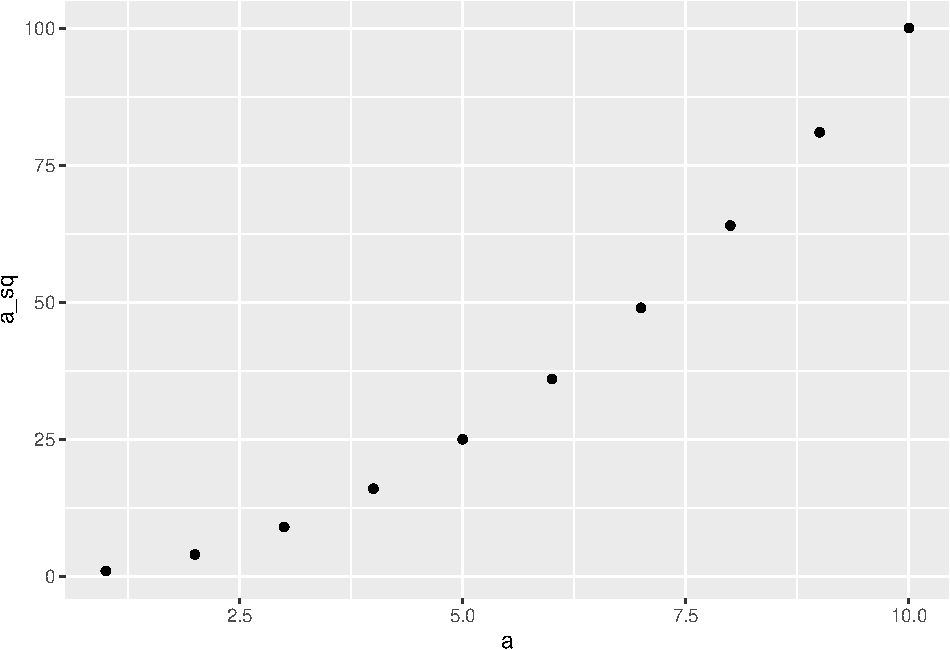
\includegraphics{main_files/figure-latex/unnamed-chunk-136-1.pdf}

\begin{Shaded}
\begin{Highlighting}[]
\FunctionTok{ggplot}\NormalTok{(}\AttributeTok{data =}\NormalTok{ df, }\AttributeTok{mapping =} \FunctionTok{aes}\NormalTok{(}\AttributeTok{x =}\NormalTok{ a, }\AttributeTok{y =}\NormalTok{ a\_sq)) }\SpecialCharTok{+} \FunctionTok{geom\_bar}\NormalTok{(}\AttributeTok{stat=}\StringTok{"identity"}\NormalTok{)}
\end{Highlighting}
\end{Shaded}

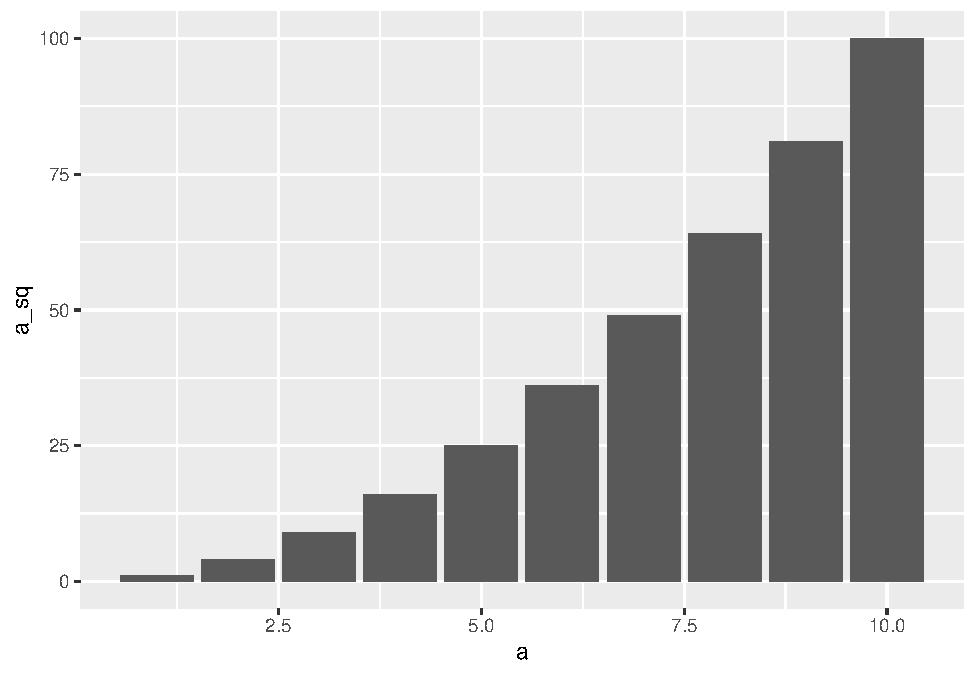
\includegraphics{main_files/figure-latex/unnamed-chunk-137-1.pdf}

\begin{Shaded}
\begin{Highlighting}[]
\FunctionTok{ggplot}\NormalTok{(}\AttributeTok{data =}\NormalTok{ df, }\AttributeTok{mapping =} \FunctionTok{aes}\NormalTok{(}\AttributeTok{x =}\NormalTok{ a\_sq, }\AttributeTok{y =}\NormalTok{ a)) }\SpecialCharTok{+} \FunctionTok{geom\_point}\NormalTok{()}
\end{Highlighting}
\end{Shaded}

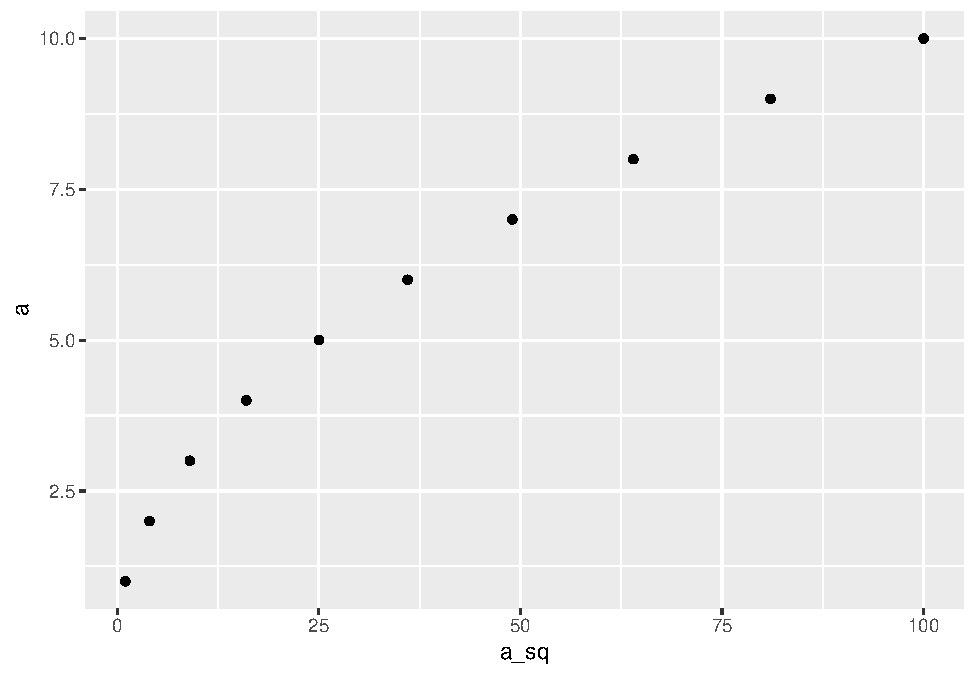
\includegraphics{main_files/figure-latex/unnamed-chunk-138-1.pdf}

\begin{Shaded}
\begin{Highlighting}[]
\FunctionTok{ggplot}\NormalTok{(}\AttributeTok{data =}\NormalTok{ df, }\AttributeTok{mapping =} \FunctionTok{aes}\NormalTok{(}\AttributeTok{x =}\NormalTok{ a\_sq, }\AttributeTok{y =}\NormalTok{ a)) }\SpecialCharTok{+} \FunctionTok{geom\_bar}\NormalTok{(}\AttributeTok{stat=}\StringTok{"identity"}\NormalTok{)}
\end{Highlighting}
\end{Shaded}

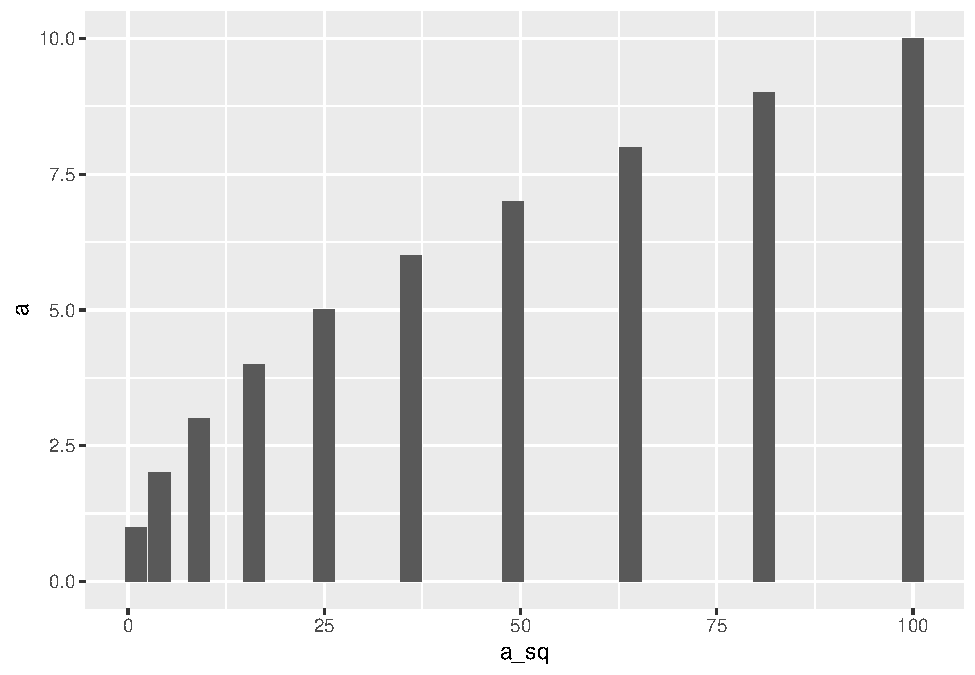
\includegraphics{main_files/figure-latex/unnamed-chunk-139-1.pdf}

\hypertarget{the-basics-of-ggplot2-1}{%
\section{The basics of ggplot2}\label{the-basics-of-ggplot2-1}}

\begin{itemize}
\item
  So what do those function calls mean?
\item
  Let's take a look at it again: This is pretty much the minimal useful plotting command in R.
\end{itemize}

\begin{Shaded}
\begin{Highlighting}[]
\FunctionTok{ggplot}\NormalTok{(}\AttributeTok{data =}\NormalTok{ df, }\AttributeTok{mapping =} \FunctionTok{aes}\NormalTok{(}\AttributeTok{x =}\NormalTok{ a, }\AttributeTok{y =}\NormalTok{ a\_sq)) }\SpecialCharTok{+} \FunctionTok{geom\_point}\NormalTok{()}
\end{Highlighting}
\end{Shaded}

\begin{itemize}
\tightlist
\item
  Each ggplot2 plot specification consists, at a minimum, of three parts:

  \begin{enumerate}
  \def\labelenumi{\arabic{enumi}.}
  \tightlist
  \item
    {the data to plot}
  \item
    {\emph{an abstract specification of the plot} (a rough mapping between variables and axes and other plot elements, such as \emph{groups}, \emph{facets}, etc.)}
  \item
    {\emph{concrete instructions on what to draw} (a specification of the actual visual elements to use)}
  \end{enumerate}
\item
  They correspond to three parts of the \texttt{ggplot()} function call

  \begin{enumerate}
  \def\labelenumi{\arabic{enumi}.}
  \tightlist
  \item
    {\textbf{data:} \texttt{data\ =\ df}}
  \item
    {\textbf{`aesthetic':} \texttt{mapping\ =\ aes(x,\ y)}}
  \item
    {\textbf{`geoms':} \texttt{+\ geom\_point()}}
  \end{enumerate}
\item
  You can read the instruction below as \emph{``Create a plot {using the data in data frame df}, {placing \texttt{a} on the x-axis and \texttt{a\_sq} on the y-axis}, {and visualize the data using points}''}.
\item
  Keep in mind that information regarding x and y axes is specified within a function called \texttt{aes()}.
\end{itemize}

\begin{Shaded}
\begin{Highlighting}[]
\FunctionTok{ggplot}\NormalTok{(}\AttributeTok{data =}\NormalTok{ df, }\AttributeTok{mapping =} \FunctionTok{aes}\NormalTok{(}\AttributeTok{x =}\NormalTok{ a, }\AttributeTok{y =}\NormalTok{ a\_sq)) }\SpecialCharTok{+} \FunctionTok{geom\_point}\NormalTok{()}
\end{Highlighting}
\end{Shaded}

\begin{itemize}
\tightlist
\item
  As an aside: A shorter way to write the same code is below, and I'll mostly use some mixed form.
\end{itemize}

\begin{Shaded}
\begin{Highlighting}[]
\FunctionTok{ggplot}\NormalTok{(df, }\FunctionTok{aes}\NormalTok{(a, a\_sq)) }\SpecialCharTok{+} \FunctionTok{geom\_point}\NormalTok{()}
\end{Highlighting}
\end{Shaded}

\hypertarget{using-lines-in-plots}{%
\section{Using lines in plots}\label{using-lines-in-plots}}

\begin{itemize}
\item
  We already know \texttt{geom\_point} and \texttt{geom\_bar}. Let's take a look at some other \emph{geoms}:.
\item
  \texttt{geom\_line} connects the (invisible, in this case) points in the plot.
\end{itemize}

\begin{Shaded}
\begin{Highlighting}[]
\FunctionTok{ggplot}\NormalTok{(df, }\FunctionTok{aes}\NormalTok{(a, a\_sq)) }\SpecialCharTok{+} \FunctionTok{geom\_line}\NormalTok{()}
\end{Highlighting}
\end{Shaded}

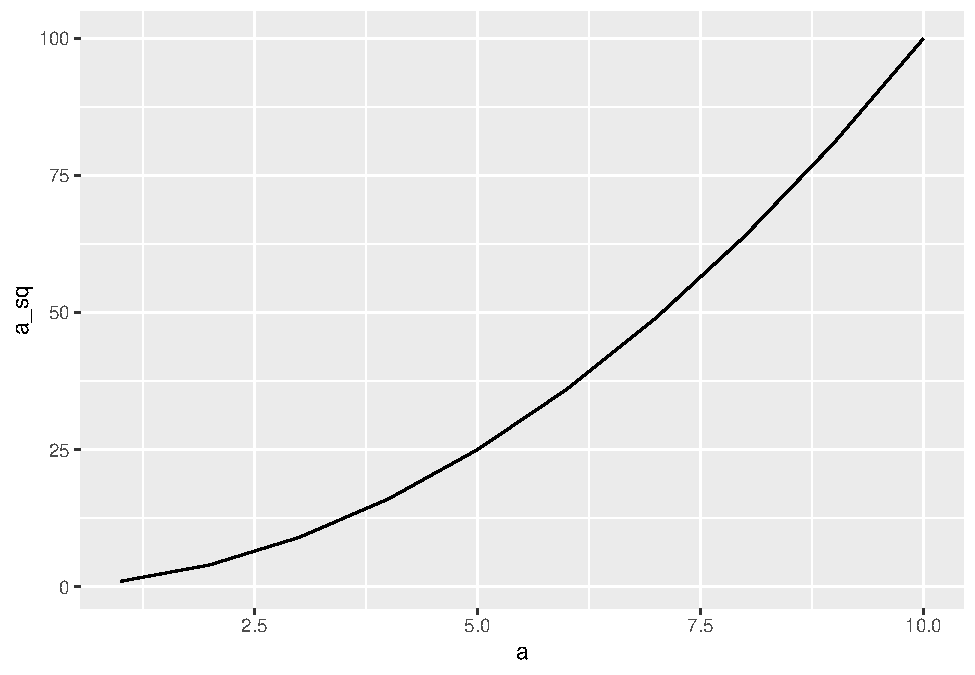
\includegraphics{main_files/figure-latex/unnamed-chunk-143-1.pdf}

\begin{itemize}
\tightlist
\item
  We can even combine geoms:
\end{itemize}

\begin{Shaded}
\begin{Highlighting}[]
\FunctionTok{ggplot}\NormalTok{(df, }\FunctionTok{aes}\NormalTok{(a, a\_sq)) }\SpecialCharTok{+} \FunctionTok{geom\_point}\NormalTok{() }\SpecialCharTok{+} \FunctionTok{geom\_line}\NormalTok{()}
\end{Highlighting}
\end{Shaded}

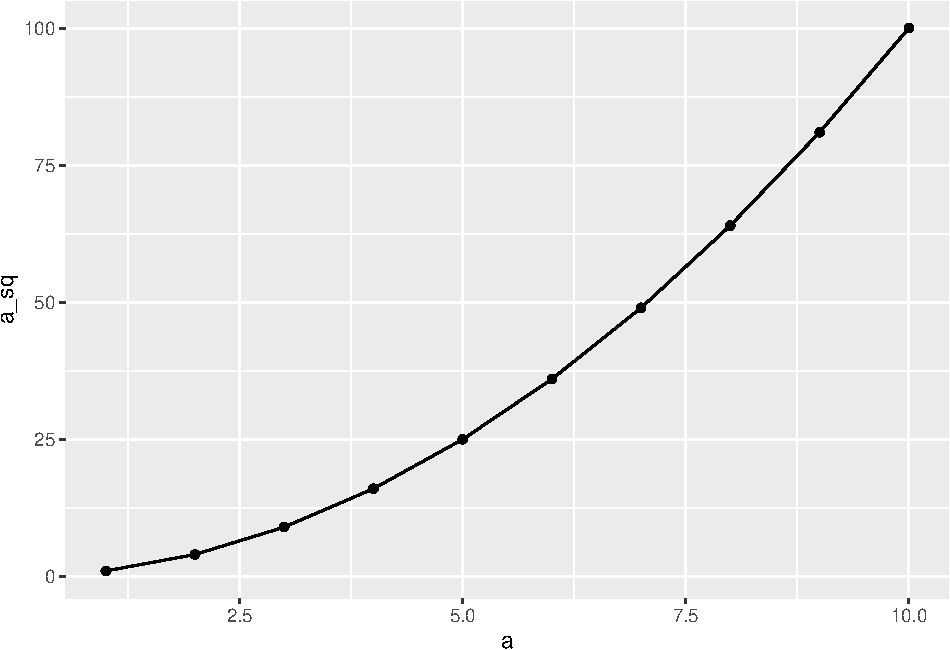
\includegraphics{main_files/figure-latex/unnamed-chunk-144-1.pdf}

\begin{itemize}
\tightlist
\item
  \ldots{} in fact, as many as we want. But there is no guarantee that the result will look good, or even make sense.
\end{itemize}

\begin{Shaded}
\begin{Highlighting}[]
\FunctionTok{ggplot}\NormalTok{(df, }\FunctionTok{aes}\NormalTok{(a, a\_sq)) }\SpecialCharTok{+} \FunctionTok{geom\_point}\NormalTok{() }\SpecialCharTok{+} \FunctionTok{geom\_line}\NormalTok{() }\SpecialCharTok{+} \FunctionTok{geom\_bar}\NormalTok{(}\AttributeTok{stat =} \StringTok{"identity"}\NormalTok{)}
\end{Highlighting}
\end{Shaded}

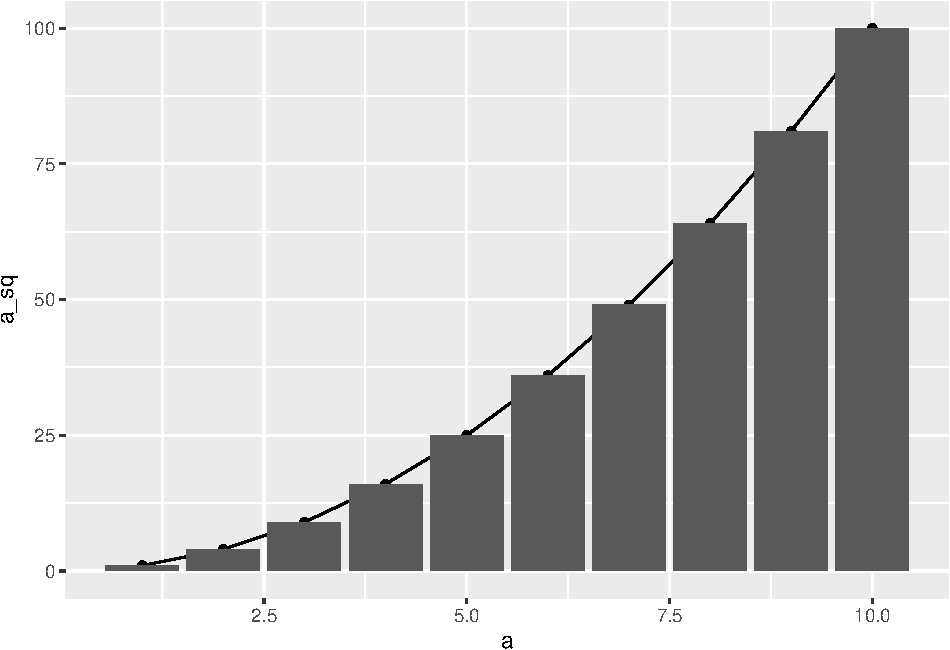
\includegraphics{main_files/figure-latex/unnamed-chunk-145-1.pdf}

\begin{itemize}
\tightlist
\item
  The order of their specification matter a little bit. Here, the line is plotted over the bars, in contrast to the previous plot.
\end{itemize}

\begin{Shaded}
\begin{Highlighting}[]
\FunctionTok{ggplot}\NormalTok{(df, }\FunctionTok{aes}\NormalTok{(a, a\_sq)) }\SpecialCharTok{+} \FunctionTok{geom\_point}\NormalTok{() }\SpecialCharTok{+} \FunctionTok{geom\_bar}\NormalTok{(}\AttributeTok{stat =} \StringTok{"identity"}\NormalTok{) }\SpecialCharTok{+} \FunctionTok{geom\_line}\NormalTok{()}
\end{Highlighting}
\end{Shaded}

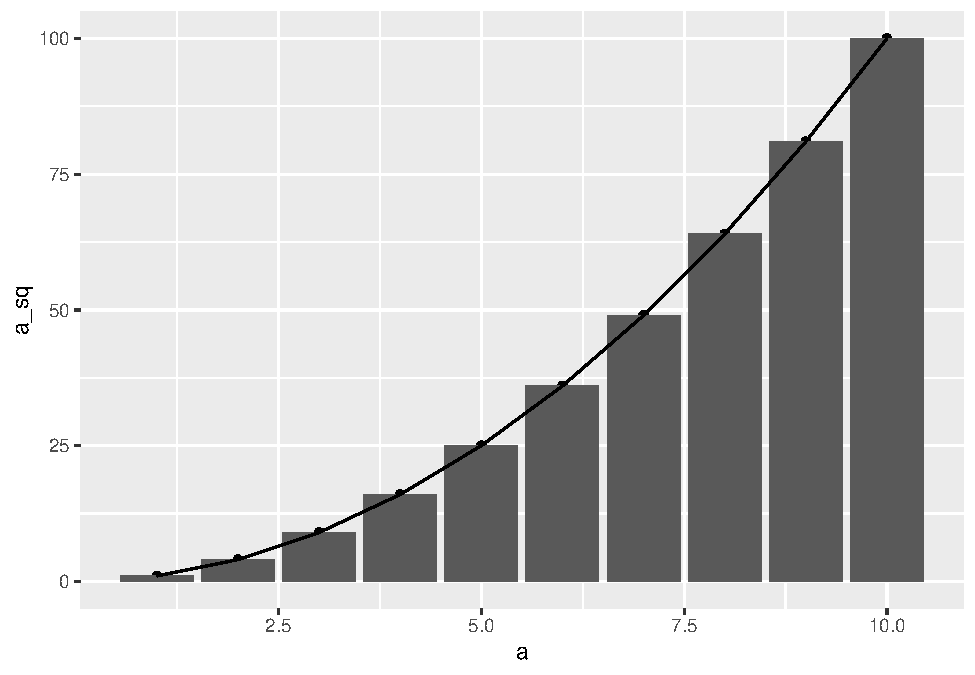
\includegraphics{main_files/figure-latex/unnamed-chunk-146-1.pdf}

\hypertarget{color-and-fill}{%
\section{Color and fill}\label{color-and-fill}}

\begin{itemize}
\item
  Relationships between two variables are usually easy to visualize, but often there is a third variable.
\item
  There are various ways for dealing with it.
\item
  Let's first try using color coding for the third variable.
\end{itemize}

\begin{Shaded}
\begin{Highlighting}[]
\FunctionTok{ggplot}\NormalTok{(df, }\FunctionTok{aes}\NormalTok{(a, a\_sq, }\AttributeTok{color =}\NormalTok{ my\_group)) }\SpecialCharTok{+} \FunctionTok{geom\_point}\NormalTok{(}\AttributeTok{stat =} \StringTok{"identity"}\NormalTok{)}
\end{Highlighting}
\end{Shaded}

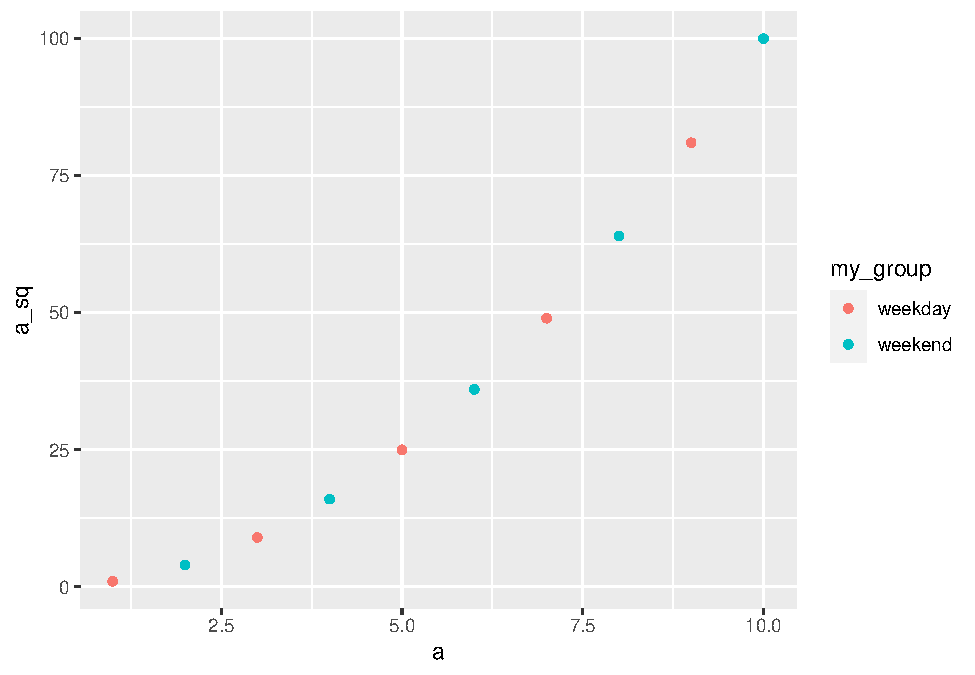
\includegraphics{main_files/figure-latex/unnamed-chunk-147-1.pdf}

\begin{itemize}
\tightlist
\item
  Let's try this with bar plots. Not at all what you expected, is it?
\end{itemize}

\begin{Shaded}
\begin{Highlighting}[]
\FunctionTok{ggplot}\NormalTok{(df, }\FunctionTok{aes}\NormalTok{(a, a\_sq, }\AttributeTok{color =}\NormalTok{ my\_group)) }\SpecialCharTok{+} \FunctionTok{geom\_bar}\NormalTok{(}\AttributeTok{stat =} \StringTok{"identity"}\NormalTok{)}
\end{Highlighting}
\end{Shaded}

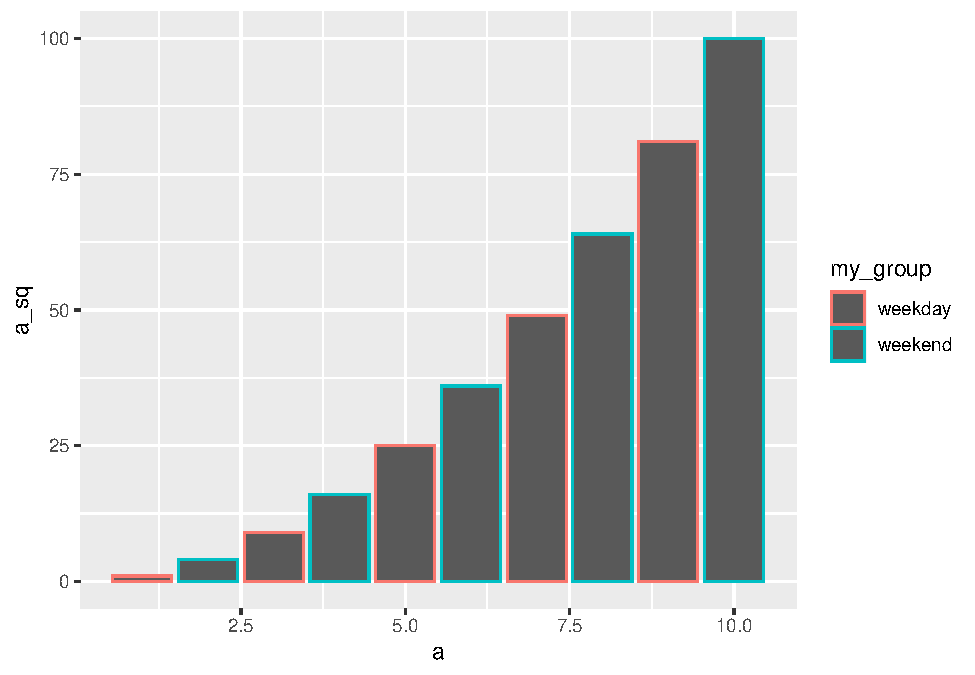
\includegraphics{main_files/figure-latex/unnamed-chunk-148-1.pdf}

\begin{itemize}
\tightlist
\item
  This is what we wanted. The right argument for bar plots is \texttt{fill}.
\end{itemize}

\begin{Shaded}
\begin{Highlighting}[]
\FunctionTok{ggplot}\NormalTok{(df, }\FunctionTok{aes}\NormalTok{(a, a\_sq, }\AttributeTok{fill =}\NormalTok{ my\_group)) }\SpecialCharTok{+} \FunctionTok{geom\_bar}\NormalTok{(}\AttributeTok{stat =} \StringTok{"identity"}\NormalTok{)}
\end{Highlighting}
\end{Shaded}

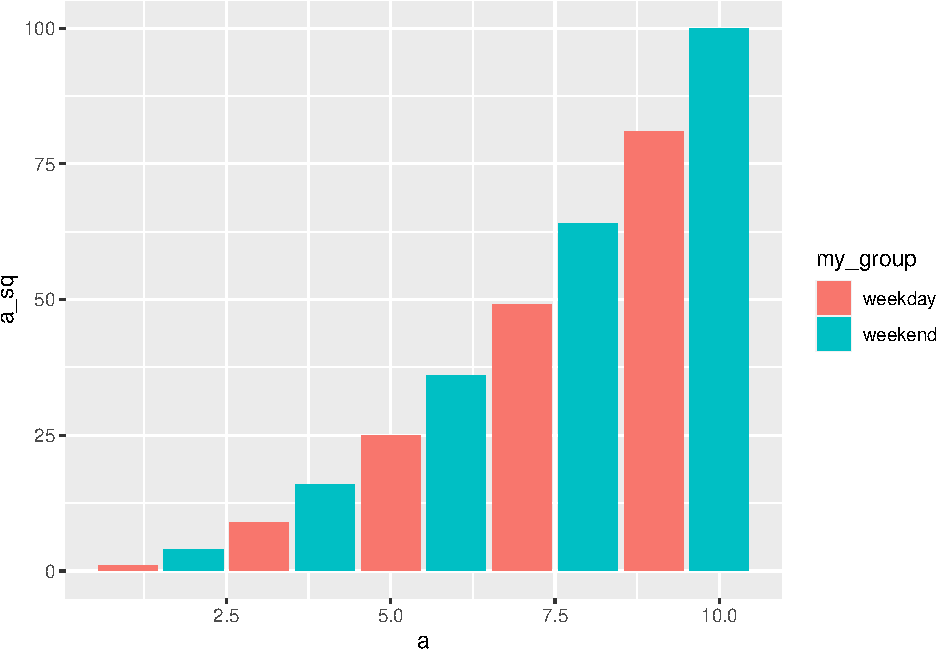
\includegraphics{main_files/figure-latex/unnamed-chunk-149-1.pdf}

\begin{itemize}
\item
  So why isn't the aesthetic argument for bar plots not also \texttt{color}?
\item
  Because geoms in ggplot2 have \texttt{fill} (the color of the inner part of the object), and a \texttt{color} (the color of the line with which they are drawn).
\item
  Points don't have a fill. (Don't ask me why.)
\item
  We can try, if you do not believe me. See that even though we specify a \texttt{fill} argument for geom\_point, \texttt{color} argument overwrites it.
\end{itemize}

\begin{Shaded}
\begin{Highlighting}[]
\FunctionTok{ggplot}\NormalTok{(df, }\FunctionTok{aes}\NormalTok{(a, a\_sq, }\AttributeTok{color =}\NormalTok{ my\_group)) }\SpecialCharTok{+} \FunctionTok{geom\_point}\NormalTok{(}\AttributeTok{size=}\DecValTok{10}\NormalTok{, }\AttributeTok{fill =} \StringTok{"black"}\NormalTok{)}
\end{Highlighting}
\end{Shaded}

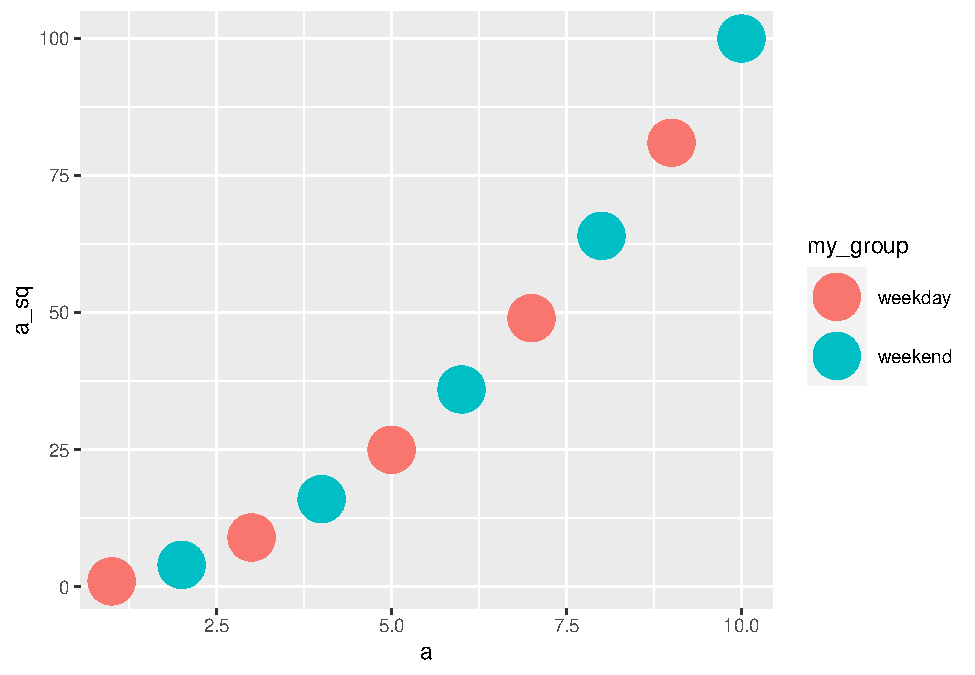
\includegraphics{main_files/figure-latex/unnamed-chunk-150-1.pdf}
- If points had a fill, we would expect the argument that comes last to overwrite the previous one.
- Bars have both fill and color arguments.

\begin{Shaded}
\begin{Highlighting}[]
\FunctionTok{ggplot}\NormalTok{(df, }\FunctionTok{aes}\NormalTok{(a, a\_sq, }\AttributeTok{fill =}\NormalTok{ my\_group)) }\SpecialCharTok{+} \FunctionTok{geom\_bar}\NormalTok{(}\AttributeTok{stat=}\StringTok{"identity"}\NormalTok{, }\AttributeTok{color =} \StringTok{"black"}\NormalTok{)}
\end{Highlighting}
\end{Shaded}

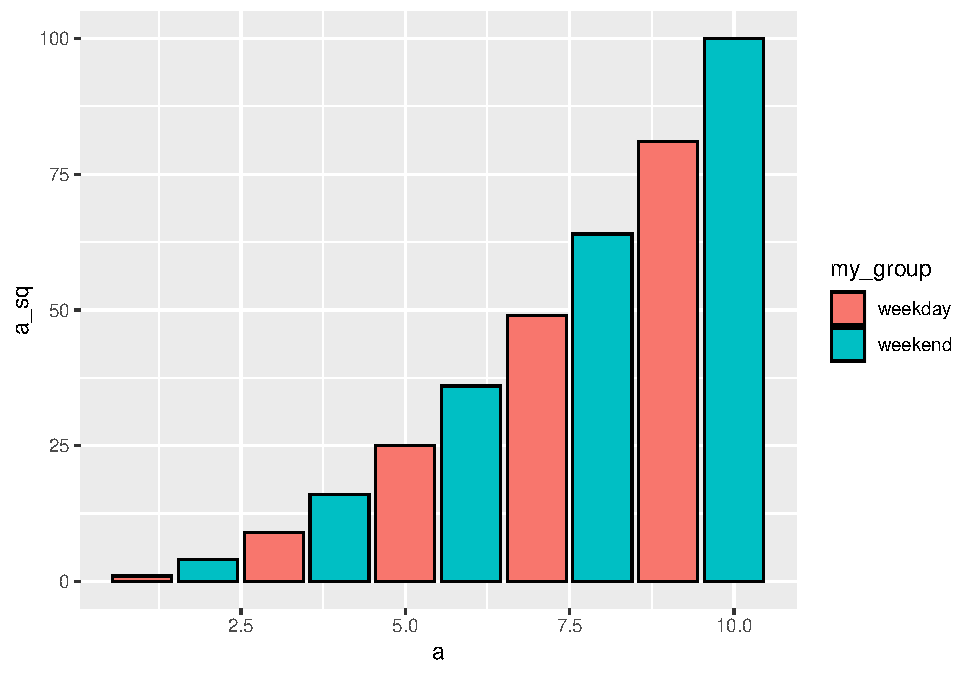
\includegraphics{main_files/figure-latex/unnamed-chunk-151-1.pdf}

\begin{Shaded}
\begin{Highlighting}[]
\FunctionTok{ggplot}\NormalTok{(df, }\FunctionTok{aes}\NormalTok{(a, a\_sq, }\AttributeTok{color =}\NormalTok{ my\_group)) }\SpecialCharTok{+} \FunctionTok{geom\_bar}\NormalTok{(}\AttributeTok{stat=}\StringTok{"identity"}\NormalTok{, }\AttributeTok{fill =} \StringTok{"black"}\NormalTok{)}
\end{Highlighting}
\end{Shaded}

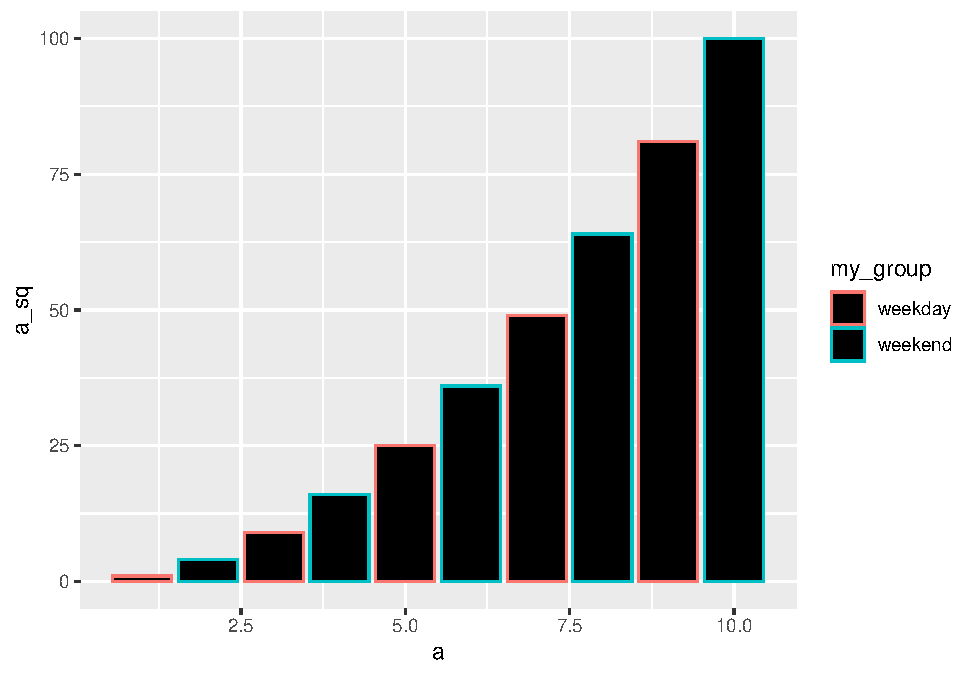
\includegraphics{main_files/figure-latex/unnamed-chunk-152-1.pdf}

\hypertarget{grouping-and-facets}{%
\section{Grouping and facets}\label{grouping-and-facets}}

\begin{itemize}
\tightlist
\item
  Color, fill, etc. implicitly group the data set into different subgroups.
\item
  You can see that better if you connect the points by lines.
\end{itemize}

\begin{Shaded}
\begin{Highlighting}[]
\FunctionTok{ggplot}\NormalTok{(df, }\FunctionTok{aes}\NormalTok{(a, a\_sq, }\AttributeTok{color =}\NormalTok{ my\_group)) }\SpecialCharTok{+} \FunctionTok{geom\_point}\NormalTok{()  }\SpecialCharTok{+} \FunctionTok{geom\_line}\NormalTok{()}
\end{Highlighting}
\end{Shaded}

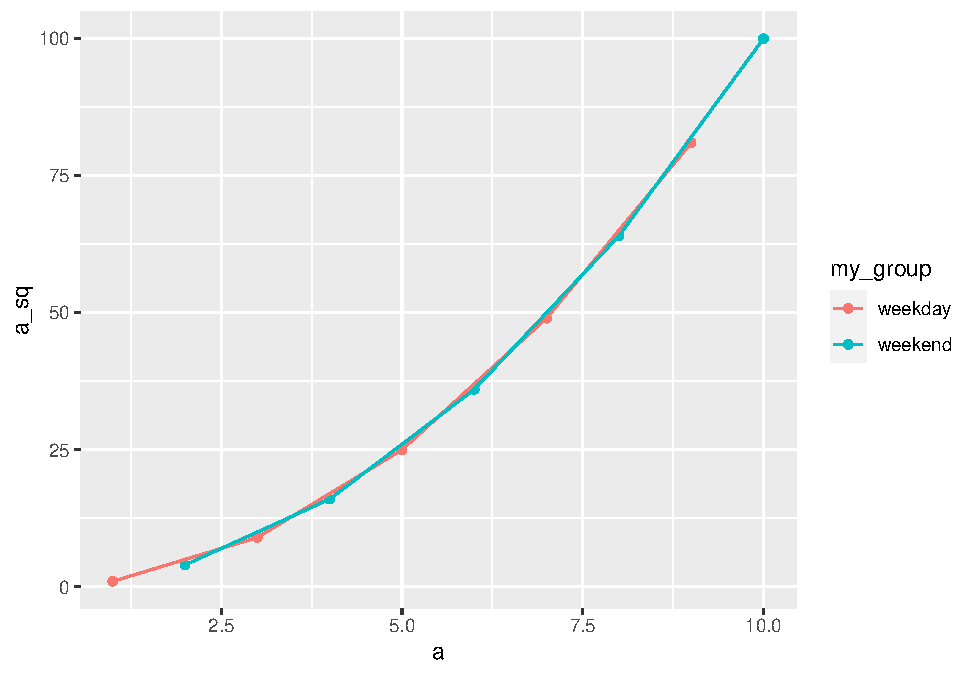
\includegraphics{main_files/figure-latex/unnamed-chunk-153-1.pdf}

\begin{itemize}
\tightlist
\item
  This can be done explicitly as well.
\end{itemize}

\begin{Shaded}
\begin{Highlighting}[]
\FunctionTok{ggplot}\NormalTok{(df, }\FunctionTok{aes}\NormalTok{(a, a\_sq, }\AttributeTok{group =}\NormalTok{ my\_group)) }\SpecialCharTok{+} \FunctionTok{geom\_point}\NormalTok{()  }\SpecialCharTok{+} \FunctionTok{geom\_line}\NormalTok{()}
\end{Highlighting}
\end{Shaded}

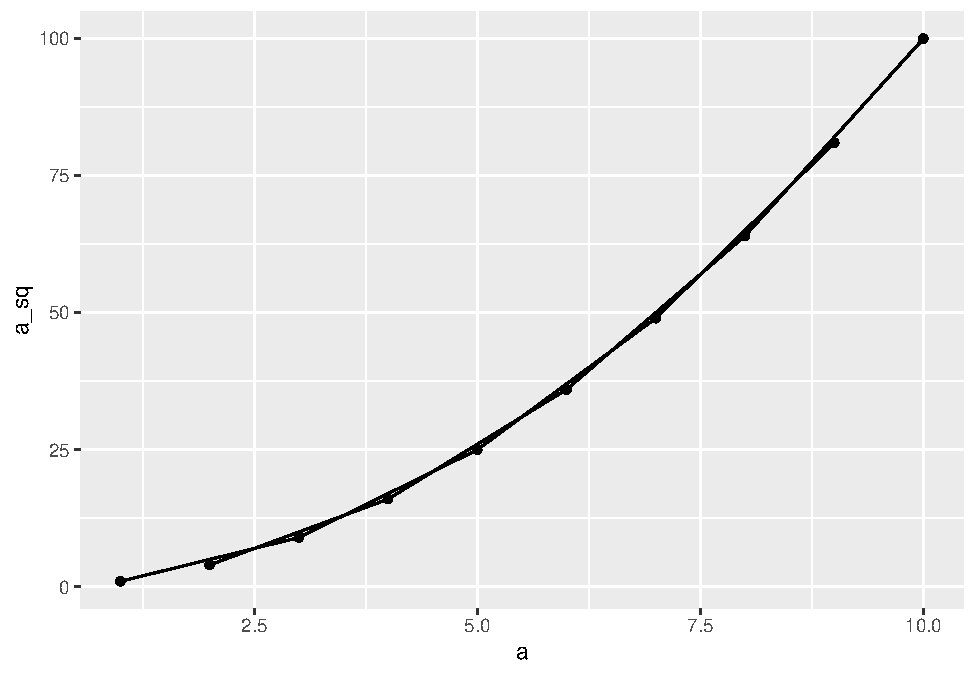
\includegraphics{main_files/figure-latex/unnamed-chunk-154-1.pdf}

\begin{itemize}
\tightlist
\item
  Now it's very hard to see which line is which, so let's at least separate it into different \textbf{facets} (aka \emph{`panels'}).
\item
  We can introduce our new facets with the function \texttt{facet\_wrap()}. Keep in mind that the grouping variable is introduced with \texttt{\textasciitilde{}}.
\item
  The name of the groups can be seen at the top of the plots.
\end{itemize}

\begin{Shaded}
\begin{Highlighting}[]
\FunctionTok{ggplot}\NormalTok{(df, }\FunctionTok{aes}\NormalTok{(a, a\_sq, }\AttributeTok{color =}\NormalTok{ my\_group)) }\SpecialCharTok{+} \FunctionTok{geom\_point}\NormalTok{()  }\SpecialCharTok{+} \FunctionTok{geom\_line}\NormalTok{() }\SpecialCharTok{+} \FunctionTok{facet\_wrap}\NormalTok{(}\SpecialCharTok{\textasciitilde{}}\NormalTok{my\_group)}
\end{Highlighting}
\end{Shaded}

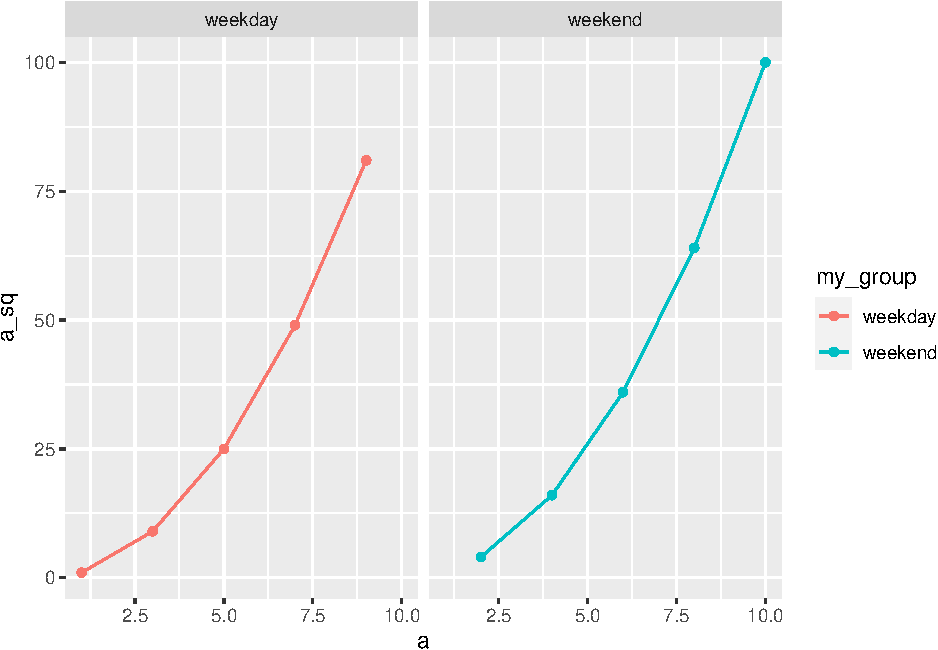
\includegraphics{main_files/figure-latex/unnamed-chunk-155-1.pdf}

\hypertarget{descriptive-statistics}{%
\chapter{Descriptive Statistics}\label{descriptive-statistics}}

Anytime you have some data, one of the first tasks you need to do is to find ways to summarize your data neatly. Raw data by itself will not make much sense. So, you want to calculate some summary statistics that describes your data. This is \textbf{descriptive statistics} (as opposed to \textbf{inferential statistics}).

Let us start with a simple dataset about the mammalian sleep hours.

\begin{Shaded}
\begin{Highlighting}[]
\FunctionTok{library}\NormalTok{(tidyverse)}
\FunctionTok{library}\NormalTok{(magrittr)}
\FunctionTok{library}\NormalTok{(lsr)}
\NormalTok{mammalian\_sleep }\OtherTok{\textless{}{-}} 
      \FunctionTok{read\_csv}\NormalTok{(}\StringTok{"./data/msleep\_ggplot2.csv"}\NormalTok{) }\SpecialCharTok{\%\textgreater{}\%} 
      \FunctionTok{select}\NormalTok{(name, sleep\_total, bodywt) }\SpecialCharTok{\%\textgreater{}\%}
      \FunctionTok{rename}\NormalTok{(}\AttributeTok{sleep\_total\_h =}\NormalTok{ sleep\_total, }\AttributeTok{bodywt\_kg =}\NormalTok{ bodywt) }\SpecialCharTok{\%\textgreater{}\%}
      \FunctionTok{mutate}\NormalTok{(}\AttributeTok{sleep\_total\_h =} \FunctionTok{round}\NormalTok{(sleep\_total\_h) )}
\end{Highlighting}
\end{Shaded}

\begin{verbatim}
## Rows: 83 Columns: 11
## -- Column specification --------------------------------------------------------
## Delimiter: ","
## chr (5): name, genus, vore, order, conservation
## dbl (6): sleep_total, sleep_rem, sleep_cycle, awake, brainwt, bodywt
## 
## i Use `spec()` to retrieve the full column specification for this data.
## i Specify the column types or set `show_col_types = FALSE` to quiet this message.
\end{verbatim}

\begin{Shaded}
\begin{Highlighting}[]
\FunctionTok{head}\NormalTok{(mammalian\_sleep)}
\end{Highlighting}
\end{Shaded}

\begin{Shaded}
\begin{Highlighting}[]
\NormalTok{\#\# \# A tibble: 6 x 3}
\NormalTok{\#\#   name                       sleep\_total\_h bodywt\_kg}
\NormalTok{\#\#   \textless{}chr\textgreater{}                              \textless{}dbl\textgreater{}     \textless{}dbl\textgreater{}}
\NormalTok{\#\# 1 Cheetah                               12    50    }
\NormalTok{\#\# 2 Owl monkey                            17     0.48 }
\NormalTok{\#\# 3 Mountain beaver                       14     1.35 }
\NormalTok{\#\# 4 Greater short{-}tailed shrew            15     0.019}
\NormalTok{\#\# 5 Cow                                    4   600    }
\NormalTok{\#\# 6 Three{-}toed sloth                      14     3.85}
\end{Highlighting}
\end{Shaded}

\begin{itemize}
\item
  There are three variables here, \texttt{name}, \texttt{sleep\_total\_h} and \texttt{bodywt\_kg}. For each animal named in \texttt{name}, the \texttt{sleep\_total\_h} variable contains the average number of hours animals of this kind sleep per day. The variable \texttt{bodywt\_kg} contains the average weight of that animal in kg.
\item
  Let's have a look at the \texttt{sleep\_total\_h} variable:
\end{itemize}

\begin{Shaded}
\begin{Highlighting}[]
\FunctionTok{print}\NormalTok{(mammalian\_sleep}\SpecialCharTok{$}\NormalTok{sleep\_total\_h)}
\end{Highlighting}
\end{Shaded}

\begin{Shaded}
\begin{Highlighting}[]
\NormalTok{\#\#  [1] 12 17 14 15  4 14  9  7 10  3  5  9 10 12 10  8  9 17  5 18  4 20  3  3 10}
\NormalTok{\#\# [26] 11 15 12 10  2  3  6  6  8 10  3 19 10 14 14 13 12 20 15 11  8 14  8  4 10}
\NormalTok{\#\# [51] 16 10 14  9 10 11 12 14  4  6 11 18  5 13  9 10  8 11 11 17 14 16 13  9  9}
\NormalTok{\#\# [76] 16  4 16  9  5  6 12 10}
\end{Highlighting}
\end{Shaded}

\begin{itemize}
\tightlist
\item
  This output doesn't make it easy to get a sense of what the data are actually saying. Just ``looking at the data'' isn't a terribly effective way of understanding data. In order to get some idea about what's going on, we need to calculate some descriptive statistics and draw some nice pictures.
\end{itemize}

\begin{Shaded}
\begin{Highlighting}[]
\FunctionTok{ggplot}\NormalTok{(mammalian\_sleep, }\FunctionTok{aes}\NormalTok{(sleep\_total\_h)) }\SpecialCharTok{+}
        \FunctionTok{geom\_histogram}\NormalTok{(}\AttributeTok{binwidth=}\DecValTok{1}\NormalTok{,}
                       \AttributeTok{color =} \StringTok{\textquotesingle{}black\textquotesingle{}}\NormalTok{,}
                       \AttributeTok{fill =} \StringTok{\textquotesingle{}lightblue\textquotesingle{}}\NormalTok{)}
\end{Highlighting}
\end{Shaded}

\begin{figure}
\centering
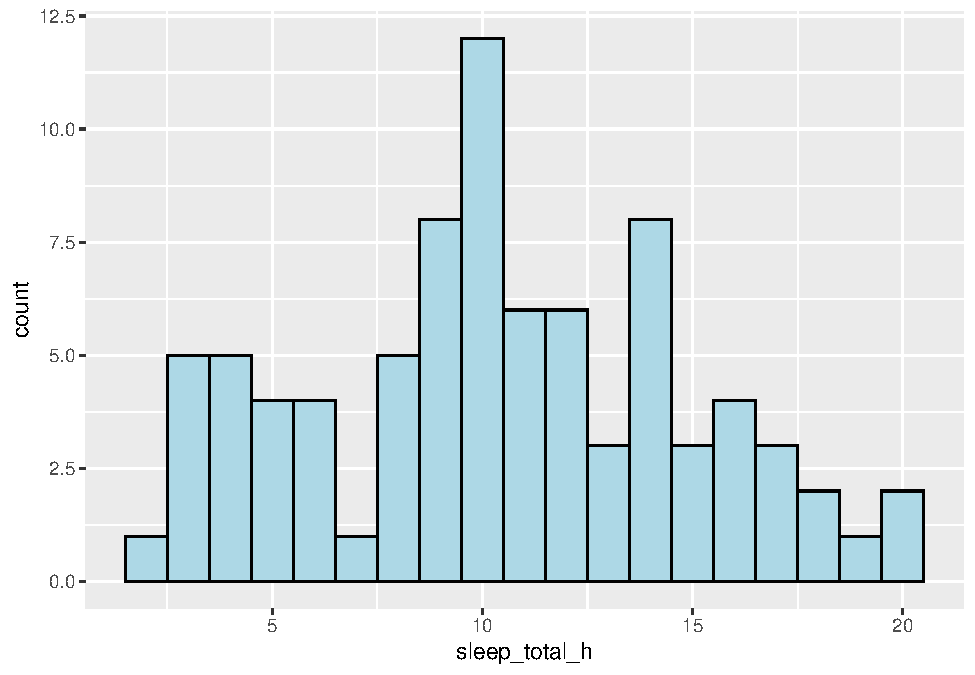
\includegraphics{main_files/figure-latex/histogram1-1.pdf}
\caption{\label{fig:histogram1}A histogram of the average amount of sleep by animal (the \texttt{sleep\_total\_h} variable). As you might expect, the larger the margin the less frequently you tend to see it.}
\end{figure}

\hypertarget{distributions}{%
\section{Distributions}\label{distributions}}

Let us see a couple more data examples to get a sense of what data might look like in the wild. First, let us generate some random data with a \textbf{uniform distribution} using the \texttt{runif()} function.

\begin{Shaded}
\begin{Highlighting}[]
\NormalTok{uniform }\OtherTok{\textless{}{-}} \FunctionTok{as\_tibble\_col}\NormalTok{(}\FunctionTok{runif}\NormalTok{(}\DecValTok{120}\NormalTok{, }\AttributeTok{min =} \DecValTok{1}\NormalTok{, }\AttributeTok{max =} \DecValTok{6}\NormalTok{),}\AttributeTok{column\_name =} \StringTok{"some\_value"}\NormalTok{)}

\NormalTok{uniform}
\end{Highlighting}
\end{Shaded}

\begin{Shaded}
\begin{Highlighting}[]
\NormalTok{\#\# \# A tibble: 120 x 1}
\NormalTok{\#\#    some\_value}
\NormalTok{\#\#         \textless{}dbl\textgreater{}}
\NormalTok{\#\#  1       2.23}
\NormalTok{\#\#  2       1.21}
\NormalTok{\#\#  3       2.64}
\NormalTok{\#\#  4       5.77}
\NormalTok{\#\#  5       5.45}
\NormalTok{\#\#  6       4.46}
\NormalTok{\#\#  7       4.20}
\NormalTok{\#\#  8       5.97}
\NormalTok{\#\#  9       4.28}
\NormalTok{\#\# 10       4.54}
\NormalTok{\#\# \# ... with 110 more rows}
\end{Highlighting}
\end{Shaded}

Let us plot the uniformly distributed data using a histogram.

\begin{Shaded}
\begin{Highlighting}[]
\FunctionTok{ggplot}\NormalTok{(uniform, }\FunctionTok{aes}\NormalTok{(some\_value)) }\SpecialCharTok{+}
        \FunctionTok{geom\_histogram}\NormalTok{(}\AttributeTok{binwidth=}\FloatTok{0.5}\NormalTok{,}\AttributeTok{boundary=}\DecValTok{0}\NormalTok{,}
                       \AttributeTok{color =} \StringTok{\textquotesingle{}black\textquotesingle{}}\NormalTok{,}
                       \AttributeTok{fill =} \StringTok{\textquotesingle{}lightblue\textquotesingle{}}\NormalTok{)}
\end{Highlighting}
\end{Shaded}

\begin{figure}
\centering
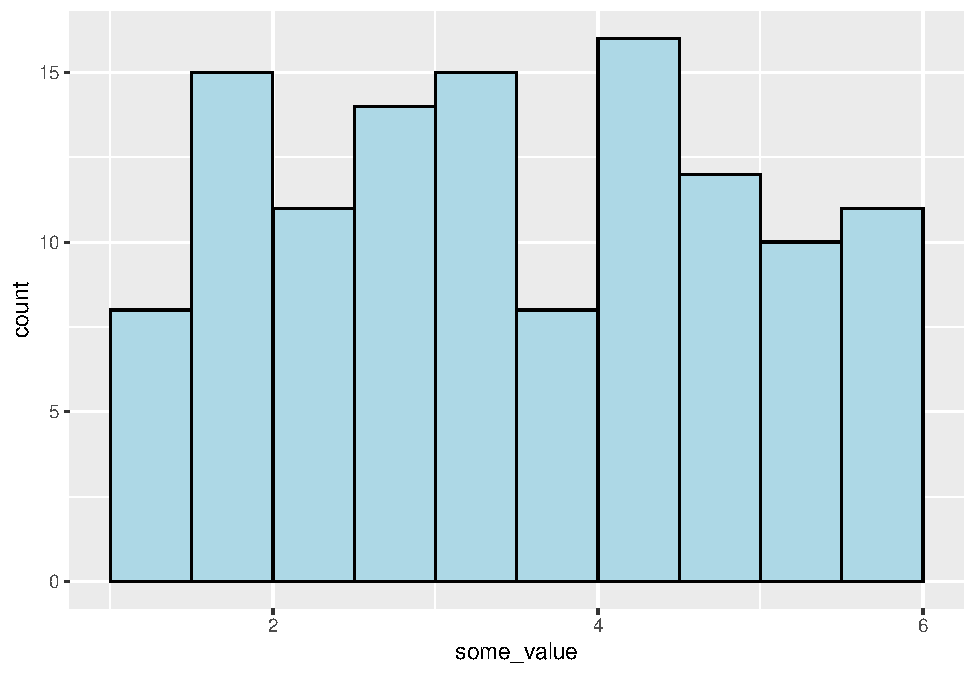
\includegraphics{main_files/figure-latex/histogram2-1.pdf}
\caption{\label{fig:histogram2}Histogram of a uniform distribution.}
\end{figure}

This looks good but it doesn't make as much intuitive sense as we'd like. Let us tweak this slightly. Assume that you have a fair dice with 6 sides. So, whenever we roll the dice, each side has an equal probability (i.e.~1/6). Let us simulate this. The data is going to be very similar, except that this time we will need \textbf{discrete} values rather than \textbf{continuous} values. For that, we need to use the \texttt{rdunif()} function which generates random values with a discrete uniform distribution.

\begin{Shaded}
\begin{Highlighting}[]
\NormalTok{uniform }\OtherTok{\textless{}{-}} \FunctionTok{as\_tibble\_col}\NormalTok{(}\FunctionTok{rdunif}\NormalTok{(}\DecValTok{120}\NormalTok{, }\DecValTok{6}\NormalTok{, }\DecValTok{1}\NormalTok{), }\AttributeTok{column\_name=}\StringTok{"dice\_value"}\NormalTok{)}
\NormalTok{uniform}
\end{Highlighting}
\end{Shaded}

\begin{Shaded}
\begin{Highlighting}[]
\NormalTok{\#\# \# A tibble: 120 x 1}
\NormalTok{\#\#    dice\_value}
\NormalTok{\#\#         \textless{}dbl\textgreater{}}
\NormalTok{\#\#  1          2}
\NormalTok{\#\#  2          2}
\NormalTok{\#\#  3          6}
\NormalTok{\#\#  4          4}
\NormalTok{\#\#  5          4}
\NormalTok{\#\#  6          6}
\NormalTok{\#\#  7          1}
\NormalTok{\#\#  8          6}
\NormalTok{\#\#  9          6}
\NormalTok{\#\# 10          6}
\NormalTok{\#\# \# ... with 110 more rows}
\end{Highlighting}
\end{Shaded}

\begin{Shaded}
\begin{Highlighting}[]
\FunctionTok{ggplot}\NormalTok{(uniform, }\FunctionTok{aes}\NormalTok{(dice\_value)) }\SpecialCharTok{+}
  \FunctionTok{geom\_bar}\NormalTok{(}\AttributeTok{color =} \StringTok{\textquotesingle{}black\textquotesingle{}}\NormalTok{,}
           \AttributeTok{fill =} \StringTok{\textquotesingle{}lightblue\textquotesingle{}}\NormalTok{)}
\end{Highlighting}
\end{Shaded}

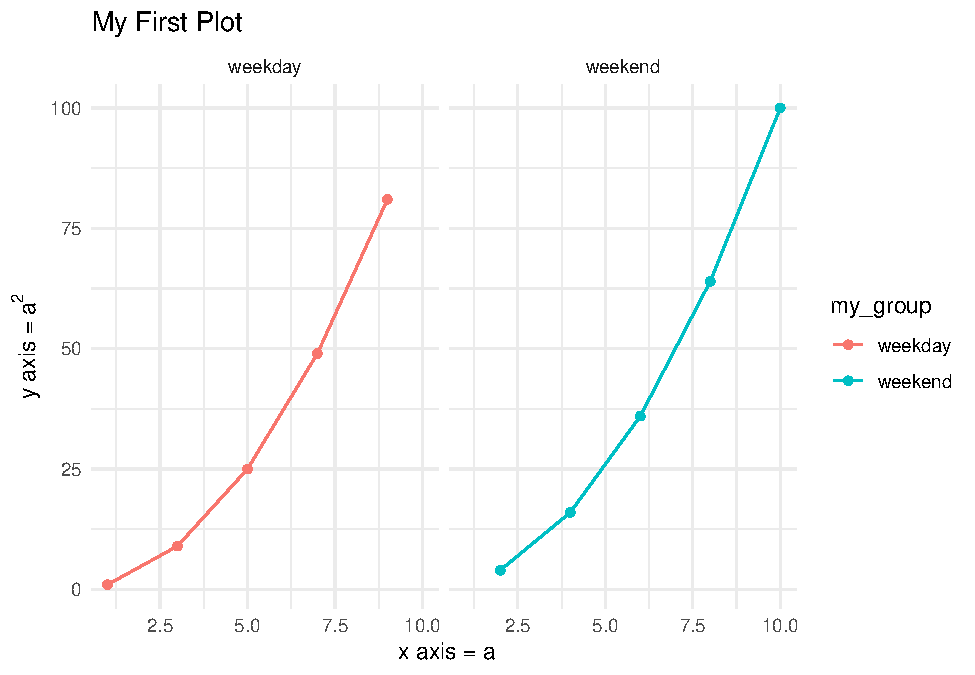
\includegraphics{main_files/figure-latex/unnamed-chunk-159-1.pdf}

\begin{verbatim}
Just a quick point to think about. Why did we use a histogram for the 
continuous uniform distribution and a bar graph for a discrete one? 
Also, why didn't we use the **stat="identity"** argument in the bar graph?
\end{verbatim}

Now, let us generate some random data with a \textbf{normal distribution} using the \texttt{rnorm}()` function.

\begin{Shaded}
\begin{Highlighting}[]
\NormalTok{normal }\OtherTok{\textless{}{-}} \FunctionTok{as\_tibble}\NormalTok{(}\FunctionTok{rnorm}\NormalTok{(}\DecValTok{160}\NormalTok{))}
\end{Highlighting}
\end{Shaded}

Let us plot the normally distributed data using a histogram.

\begin{Shaded}
\begin{Highlighting}[]
\FunctionTok{ggplot}\NormalTok{(normal, }\FunctionTok{aes}\NormalTok{(value)) }\SpecialCharTok{+}
        \FunctionTok{geom\_histogram}\NormalTok{(}\AttributeTok{binwidth=}\FloatTok{0.2}\NormalTok{,}
                       \AttributeTok{color =} \StringTok{\textquotesingle{}black\textquotesingle{}}\NormalTok{,}
                       \AttributeTok{fill =} \StringTok{\textquotesingle{}lightblue\textquotesingle{}}\NormalTok{)}
\end{Highlighting}
\end{Shaded}

\begin{figure}
\centering
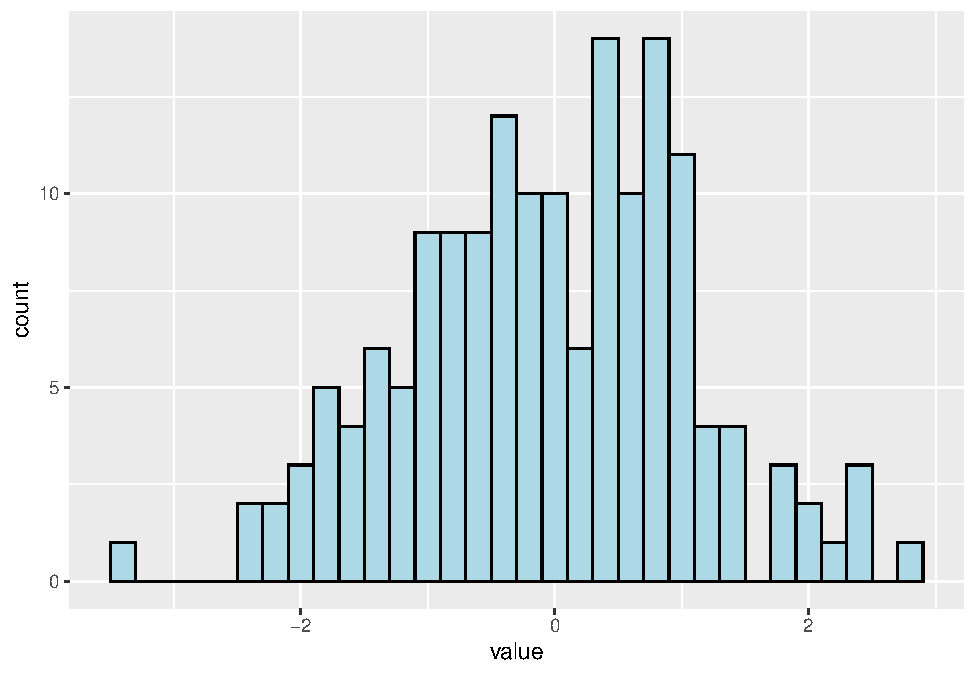
\includegraphics{main_files/figure-latex/histogram3-1.pdf}
\caption{\label{fig:histogram3}Histogram of a normal distribution.}
\end{figure}

Here's another one where we provide the \textbf{mean} and \textbf{standard deviation} parameteres.

\begin{Shaded}
\begin{Highlighting}[]
\NormalTok{normal2 }\OtherTok{\textless{}{-}} \FunctionTok{as\_tibble}\NormalTok{(}\FunctionTok{rnorm}\NormalTok{(}\DecValTok{160}\NormalTok{, }\AttributeTok{mean =} \DecValTok{8}\NormalTok{, }\AttributeTok{sd=} \FloatTok{0.5}\NormalTok{))}
\end{Highlighting}
\end{Shaded}

Let us plot the seconf normally distributed data using a histogram.

\begin{Shaded}
\begin{Highlighting}[]
\FunctionTok{ggplot}\NormalTok{(normal2, }\FunctionTok{aes}\NormalTok{(value)) }\SpecialCharTok{+}
        \FunctionTok{geom\_histogram}\NormalTok{(}\AttributeTok{binwidth=}\FloatTok{0.2}\NormalTok{,}
                       \AttributeTok{color =} \StringTok{\textquotesingle{}black\textquotesingle{}}\NormalTok{,}
                       \AttributeTok{fill =} \StringTok{\textquotesingle{}steelblue\textquotesingle{}}\NormalTok{)}
\end{Highlighting}
\end{Shaded}

\begin{figure}
\centering
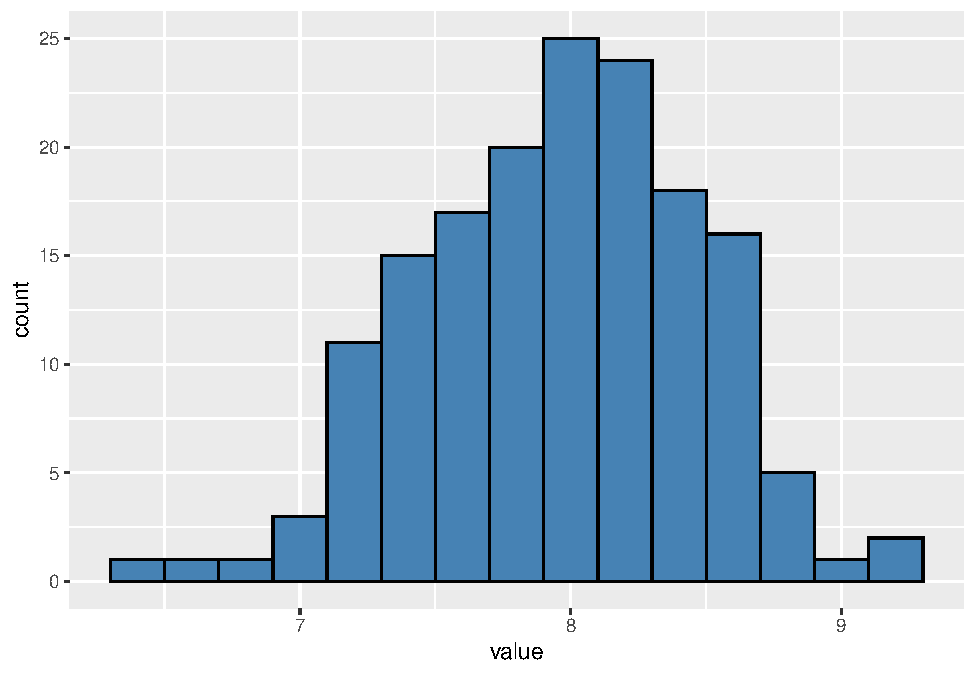
\includegraphics{main_files/figure-latex/histogram4-1.pdf}
\caption{\label{fig:histogram4}Histogram of a normal distribution.}
\end{figure}

Finally, let us plot both of the normally distributed data on the same plot to see them side by side.

\begin{Shaded}
\begin{Highlighting}[]
\FunctionTok{ggplot}\NormalTok{(normal, }\FunctionTok{aes}\NormalTok{(value)) }\SpecialCharTok{+}
        \FunctionTok{geom\_histogram}\NormalTok{(}\AttributeTok{binwidth=}\FloatTok{0.2}\NormalTok{,}
                       \AttributeTok{color =} \StringTok{\textquotesingle{}black\textquotesingle{}}\NormalTok{,}
                       \AttributeTok{fill =} \StringTok{\textquotesingle{}lightblue\textquotesingle{}}\NormalTok{) }\SpecialCharTok{+}
          \FunctionTok{geom\_histogram}\NormalTok{(}\AttributeTok{data=}\NormalTok{normal2, }\AttributeTok{binwidth=}\FloatTok{0.2}\NormalTok{,}\AttributeTok{boundary=}\DecValTok{0}\NormalTok{,}
                       \AttributeTok{color =} \StringTok{\textquotesingle{}black\textquotesingle{}}\NormalTok{,}
                       \AttributeTok{fill =} \StringTok{\textquotesingle{}steelblue\textquotesingle{}}\NormalTok{)}
\end{Highlighting}
\end{Shaded}

\begin{figure}
\centering
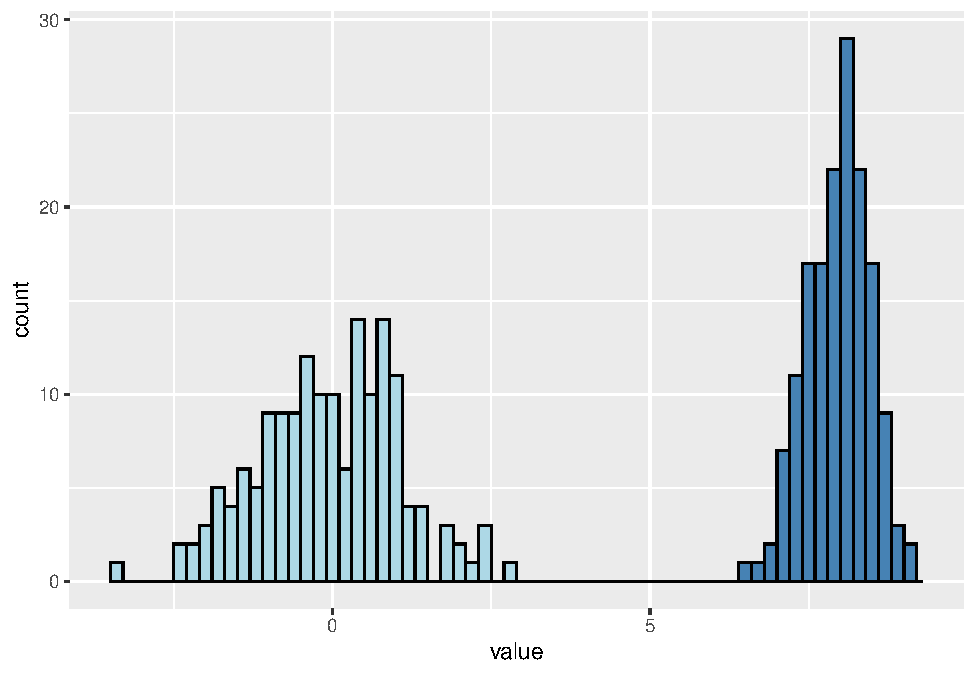
\includegraphics{main_files/figure-latex/histogram5-1.pdf}
\caption{\label{fig:histogram5}Histogram of two normal distributions side by side.}
\end{figure}

\begin{figure}
\centering
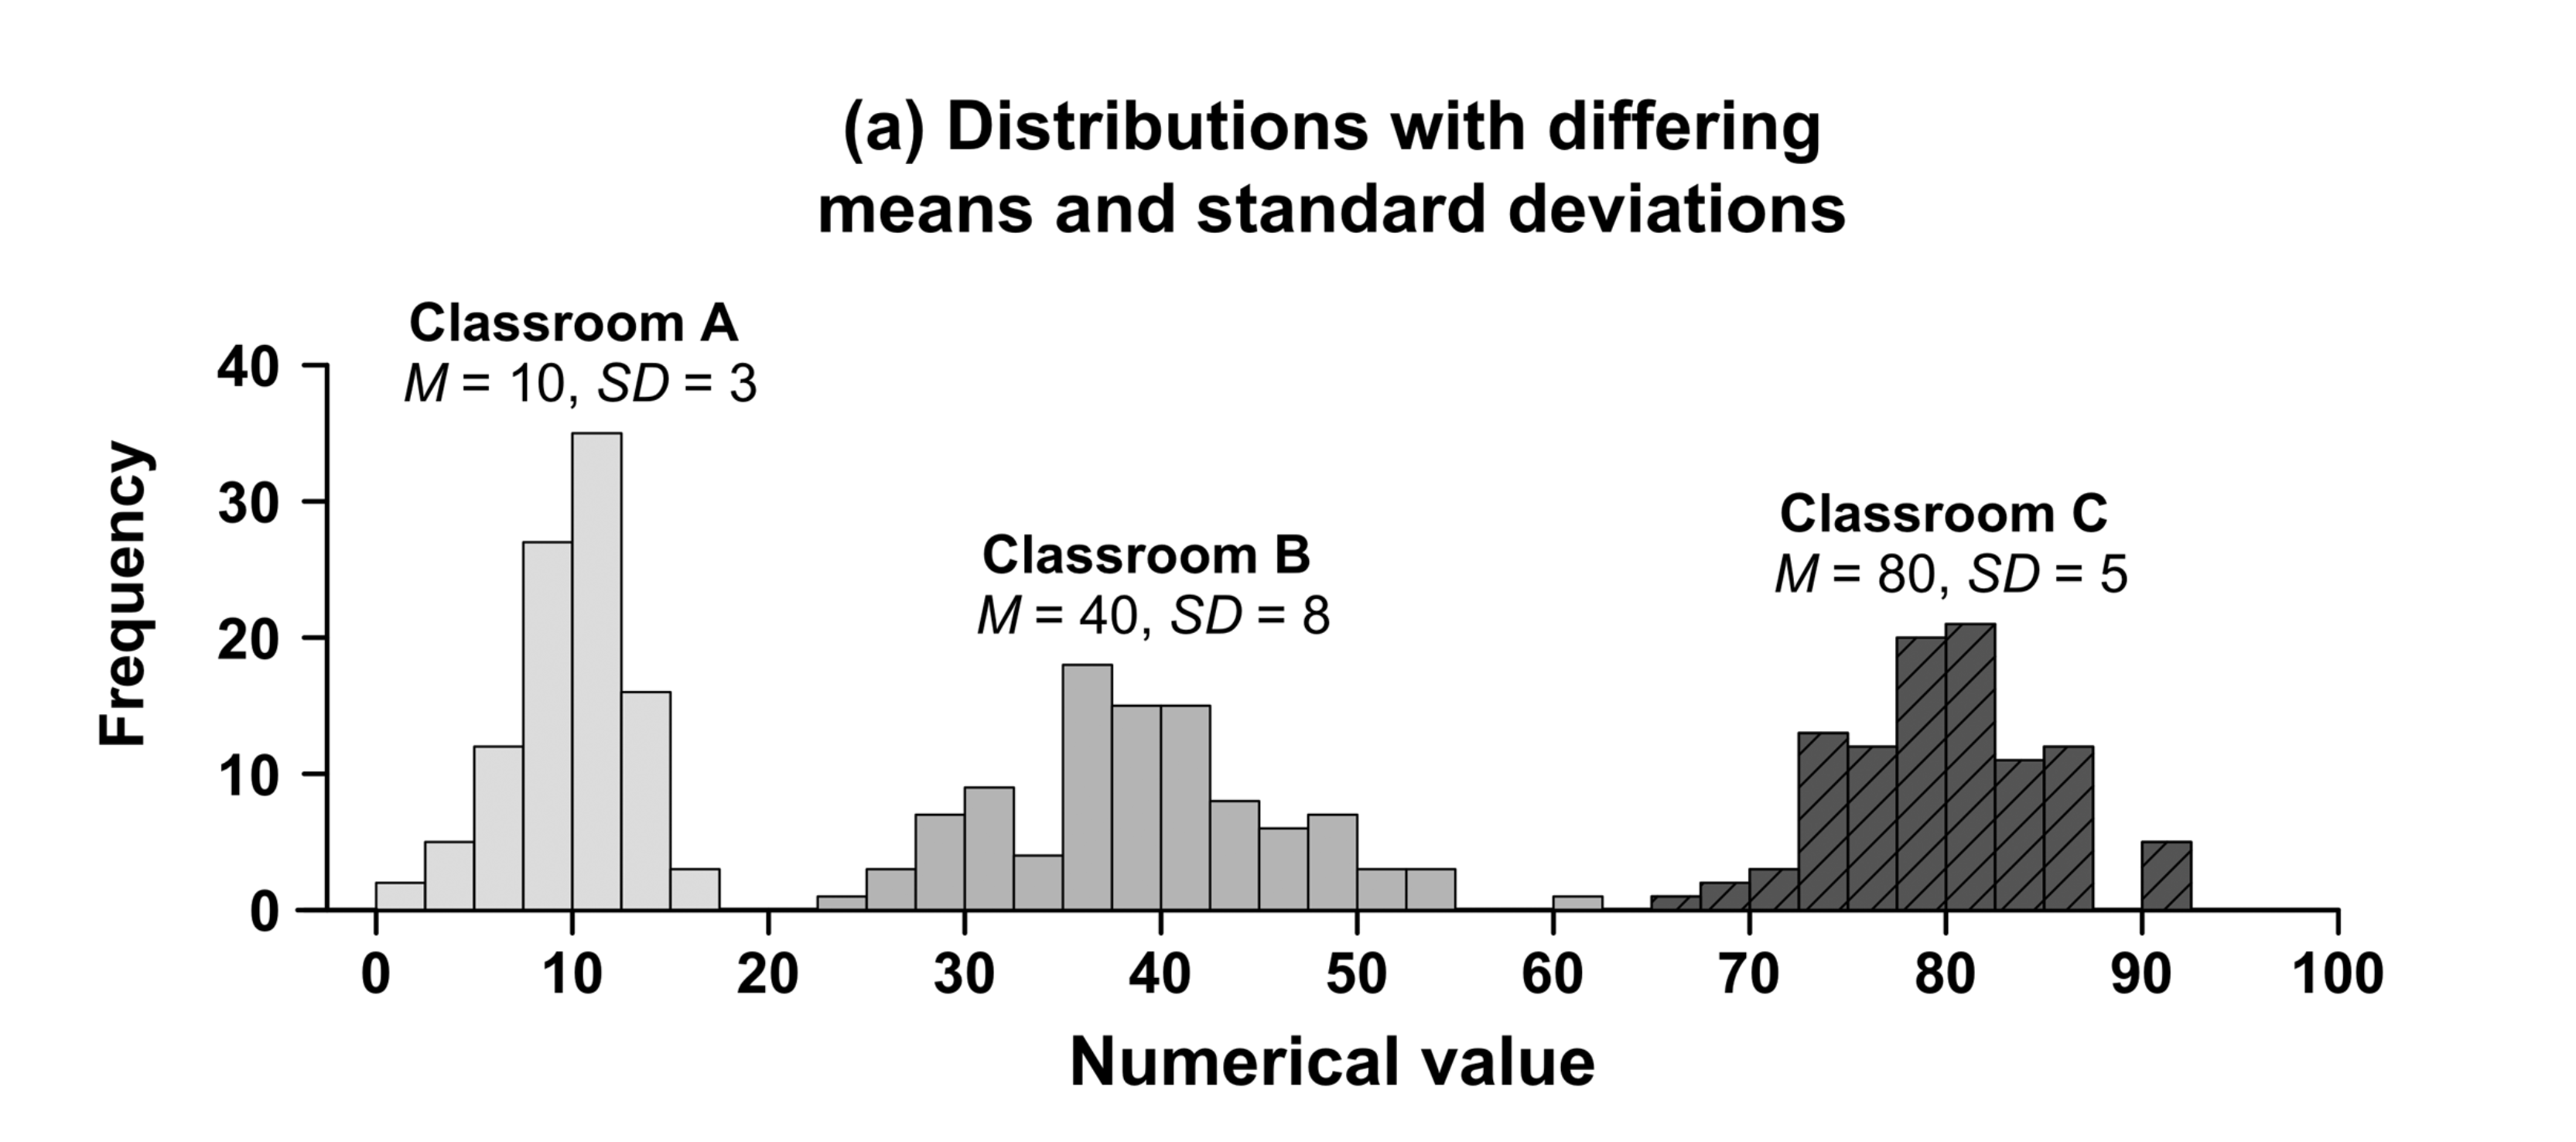
\includegraphics{./img/descriptives2/data_distribution.png}
\caption{\label{fig:normaldatadistributions}Distributions with different means and standard deviations.}
\end{figure}

\begin{figure}
\centering
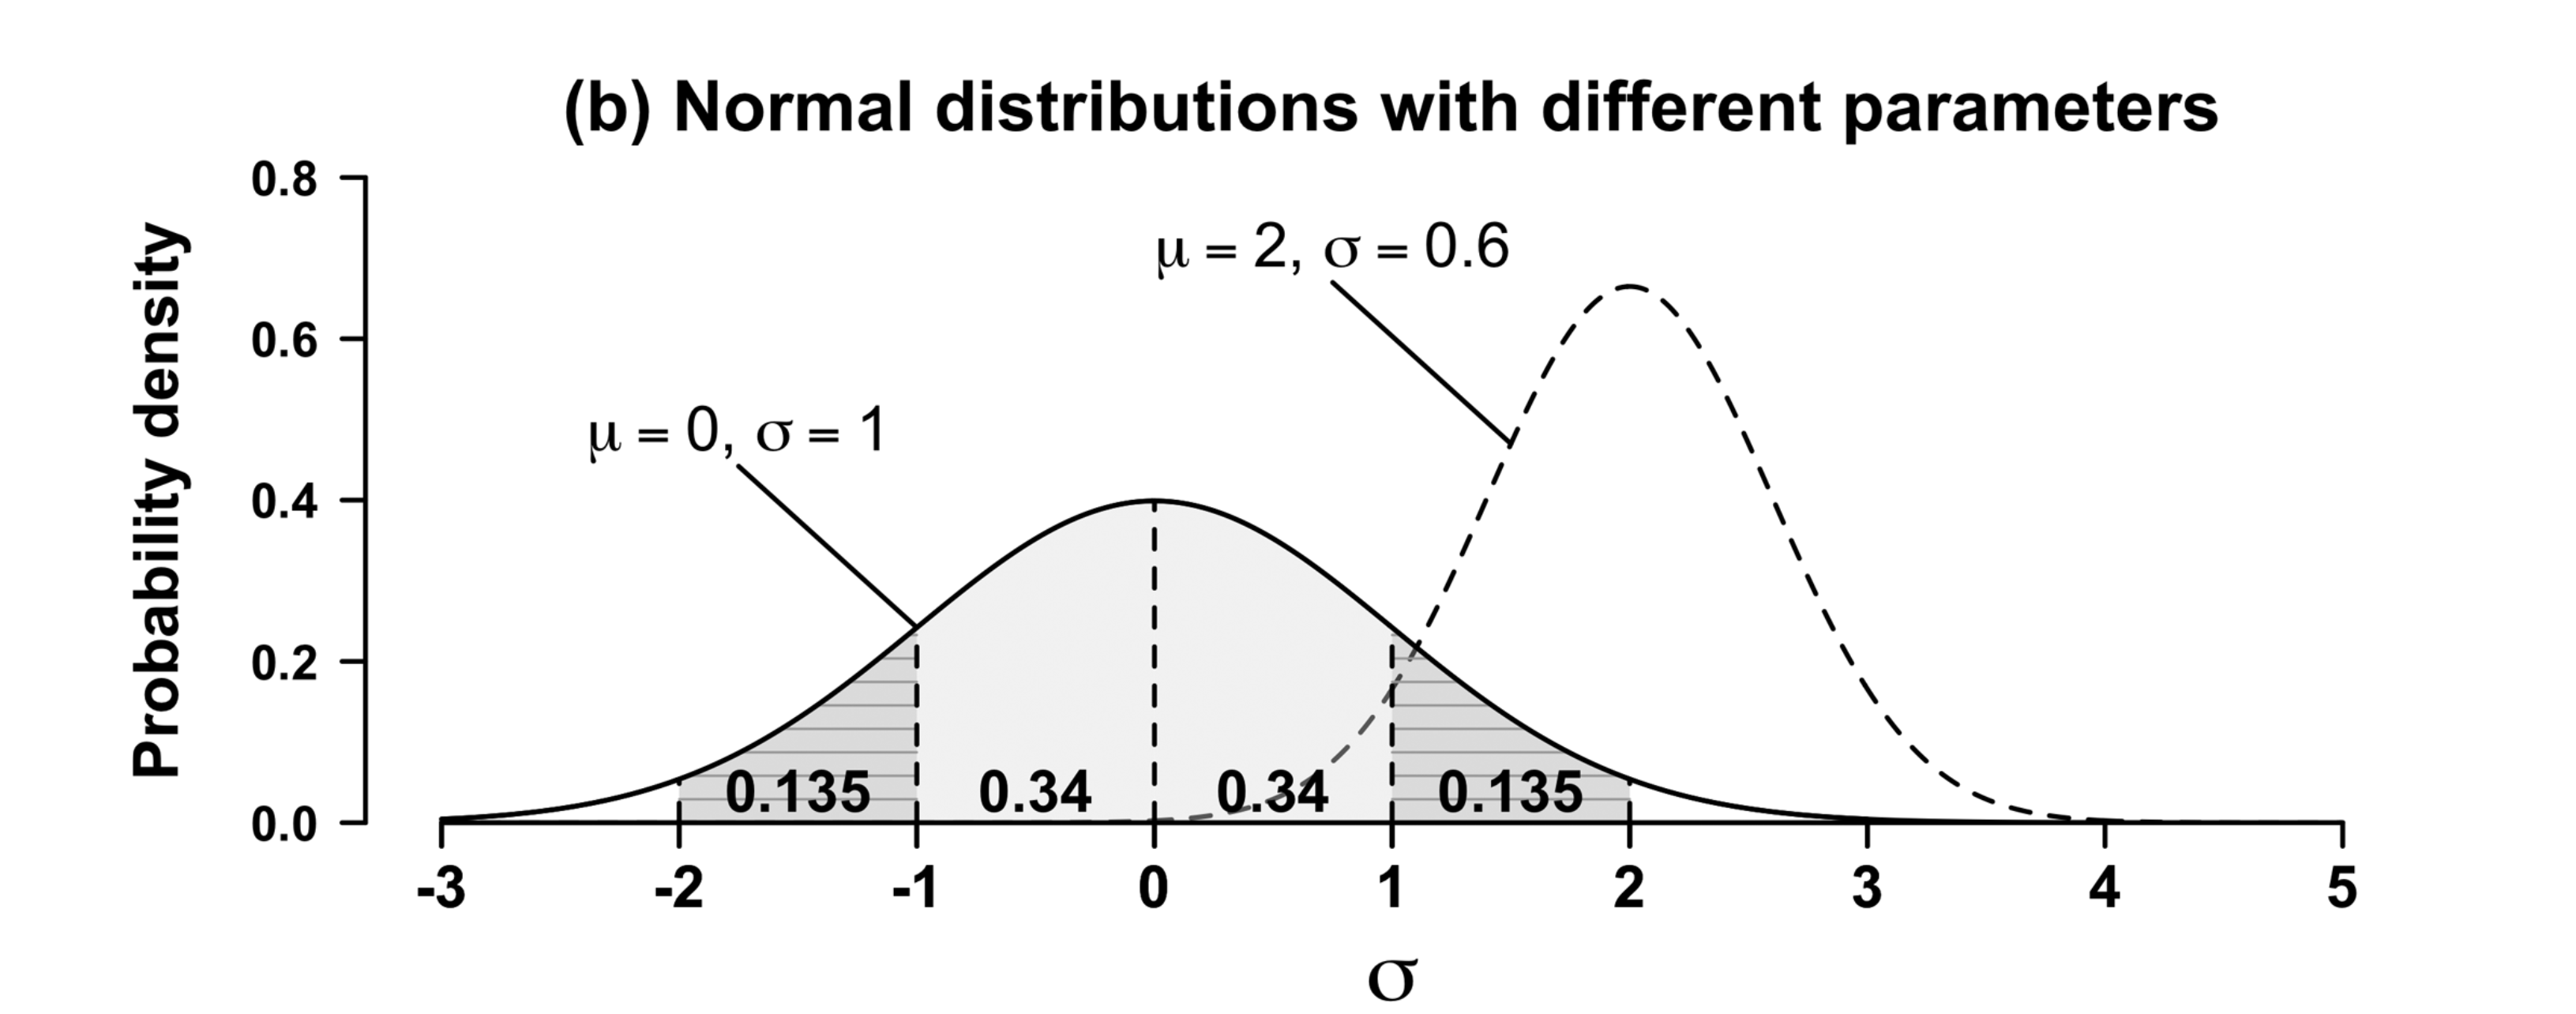
\includegraphics{./img/descriptives2/normal_distribution.png}
\caption{\label{fig:normalparameterdistributions}Distributions with different means and standard deviations. The light gray area covers the 68\% of the data and the total of the gray areas cover the 95\% of the data.}
\end{figure}

\hypertarget{centraltendency}{%
\section{Measures of central tendency}\label{centraltendency}}

Drawing pictures of the data, as I did in Figure \ref{fig:histogram1} is an excellent way to convey the ``gist'' of what the data is trying to tell you, it's often extremely useful to try to condense the data into a few simple ``summary'' statistics. In most situations, the first thing that you'll want to calculate is a measure of \textbf{\emph{central tendency}}. That is, you'd like to know something about the ``average'' or ``middle'' of your data lies. The three most commonly used measures are the \textbf{mean}, \textbf{median} and \textbf{mode}; occasionally people will also report a trimmed mean. I'll explain each of these in turn, and then discuss when each of them is useful.

\hypertarget{mean}{%
\subsection{The mean}\label{mean}}

\begin{itemize}
\item
  The \textbf{\emph{mean}} of a set of observations is just a normal, old-fashioned average: add all of the values up, and then divide by the total number of values. The first five animals' typical amount of sleep is 12 + 17 + 14 + 15 + 4, so the mean of these observations is just:
  \[
  \frac{12 + 17 + 14 + 15 + 4}{5} = \frac{62.4}{5} = 12.48
  \]
\item
  Of course, this definition of the mean isn't news to anyone: averages (i.e., means) are used so often in everyday life that this is pretty familiar stuff. However, since the concept of a mean is something that everyone already understands, I'll use this as an excuse to start introducing some of the mathematical notation that statisticians use to describe this calculation, and talk about how the calculations would be done in R.
\item
  The first piece of notation to introduce is \(N\), which we'll use to refer to the number of observations that we're averaging (in this case \(N = 5\)).
\item
  Next, we need to attach a label to the observations themselves. It's traditional to use \(X\) for this, and to use subscripts to indicate which observation we're actually talking about.
\item
  That is, we'll use \(X_1\) to refer to the first observation, \(X_2\) to refer to the second observation, and so on, all the way up to \(X_N\) for the last one. Or, to say the same thing in a slightly more abstract way, we use \(X_i\) to refer to the \(i\)-th observation. Just to make sure we're clear on the notation, the following table lists the 5 observations in the \texttt{sleep\_total\_h} variable, along with the mathematical symbol used to refer to it, and the actual value that the observation corresponds to:
\end{itemize}

\begin{tabular}{lll}
\toprule
the observation & its symbol & the observed value\\
\midrule
Cheetah (animal 1) & \$X\_1\$ & 12 hours\\
Owl monkey (animal 2) & \$X\_2\$ & 17 hours\\
Mountain beaver (animal 3) & \$X\_3\$ & 14 hours\\
Greater short-tailed shrew (animal 4) & \$X\_4\$ & 15 hours\\
Cow (animal 5) & \$X\_5\$ & 4 hours\\
\bottomrule
\end{tabular}

\begin{itemize}
\item
  Okay, now let's try to write a formula for the mean. By tradition, we use \(\bar{X}\) as the notation for the mean. So the calculation for the mean could be expressed using the following formula:
  \[
  \bar{X} = \frac{X_1 + X_2 + ... + X_{N-1} + X_N}{N}
  \]
\item
  This formula is entirely correct, but it's terribly long, so we make use of the \textbf{\emph{summation symbol}} \(\scriptstyle\sum\) to shorten it.\footnote{The choice to use \(\Sigma\) to denote summation isn't arbitrary: it's the Greek upper case letter sigma, which is the analogue of the letter S in that alphabet. Similarly, there's an equivalent symbol used to denote the multiplication of lots of numbers: because multiplications are also called ``products'', we use the \(\Pi\) symbol for this; the Greek upper case pi, which is the analogue of the letter P.} If I want to add up the first five observations, I could write out the sum the long way, \(X_1 + X_2 + X_3 + X_4 +X_5\) or I could use the summation symbol to shorten it to this:
  \[
  \sum_{i=1}^5 X_i
  \]
\item
  Taken literally, this could be read as ``the sum, taken over all \(i\) values from 1 to 5, of the value \(X_i\)''. But basically, what it means is ``add up the first five observations''. In any case, we can use this notation to write out the formula for the mean, which looks like this:
  \[
  \bar{X} = \frac{1}{N} \sum_{i=1}^N X_i 
  \]
\item
  In all honesty, I can't imagine that all this mathematical notation helps clarify the concept of the mean at all. In fact, it's really just a fancy way of writing out the same thing I said in words: add all the values up, and then divide by the total number of items. However, that's not really the reason I went into all that detail.
\item
  My goal was to try to make sure that everyone reading this book is clear on the notation that we'll be using throughout the book: \(\bar{X}\) for the mean, \(\scriptstyle\sum\) for the idea of summation, \(X_i\) for the \(i\)th observation, and \(N\) for the total number of observations.
\item
  We're going to be re-using these symbols a fair bit, so it's important that you understand them well enough to be able to ``read'' the equations, and to be able to see that it's just saying ``add up lots of things and then divide by another thing''.
\end{itemize}

\hypertarget{calculating-the-mean-in-r}{%
\subsection{Calculating the mean in R}\label{calculating-the-mean-in-r}}

Okay that's the maths, how do we get the magic computing box to do the work for us? If you really wanted to, you could do this calculation directly in R. For the first numbers, do this just by typing it in as if R were a calculator\ldots{}

\begin{Shaded}
\begin{Highlighting}[]
\NormalTok{(}\DecValTok{12} \SpecialCharTok{+} \DecValTok{17} \SpecialCharTok{+} \DecValTok{14} \SpecialCharTok{+} \DecValTok{15} \SpecialCharTok{+} \DecValTok{4}\NormalTok{) }\SpecialCharTok{/} \DecValTok{5}
\end{Highlighting}
\end{Shaded}

\begin{Shaded}
\begin{Highlighting}[]
\NormalTok{\#\# [1] 12.4}
\end{Highlighting}
\end{Shaded}

\ldots{} in which case R outputs the answer 12.4, just as if it were a calculator.

\begin{itemize}
\tightlist
\item
  However, we learned quicker ways of doing that
\end{itemize}

\begin{Shaded}
\begin{Highlighting}[]
\FunctionTok{sum}\NormalTok{( mammalian\_sleep}\SpecialCharTok{$}\NormalTok{sleep\_total\_h[}\DecValTok{1}\SpecialCharTok{:}\DecValTok{5}\NormalTok{] )}\SpecialCharTok{/} \DecValTok{5}
\end{Highlighting}
\end{Shaded}

\begin{Shaded}
\begin{Highlighting}[]
\NormalTok{\#\# [1] 12.4}
\end{Highlighting}
\end{Shaded}

\begin{Shaded}
\begin{Highlighting}[]
\CommentTok{\# or:}
\FunctionTok{mean}\NormalTok{( mammalian\_sleep}\SpecialCharTok{$}\NormalTok{sleep\_total\_h[}\DecValTok{1}\SpecialCharTok{:}\DecValTok{5}\NormalTok{] )}
\end{Highlighting}
\end{Shaded}

\begin{Shaded}
\begin{Highlighting}[]
\NormalTok{\#\# [1] 12.4}
\end{Highlighting}
\end{Shaded}

\hypertarget{median}{%
\subsection{The median}\label{median}}

\begin{itemize}
\item
  The second measure of central tendency that people use a lot is the \textbf{\emph{median}}, and it's even easier to describe than the mean. The median of a set of observations is just the middle value.
\item
  As before let's imagine we were interested only in the first 5 animals: They sleep 12, 17, 14, 15, and 4 hours respectively. To figure out the median, we sort these numbers into ascending order:
  \[
  4, 12, \color{red}{14}, 15, 17
  \]
\item
  From inspection, it's obvious that the median value of these 5 observations is 14, since that's the middle one in the sorted list (I've put it in red to make it even more obvious). Easy stuff.
\item
  But what should we do if we were interested in the first 6 animals rather than the first 5? Since the sixth animal sleeps for 14 hours, our sorted list is now:
  \[
  4, 12, \color{red}{14}, \color{red}{14}, 15, 17
  \]
\item
  That's also easy. It's still 14.
\item
  But what we do if we were interested in the first 8 animals? Here is our new sorted list.
  \[
  4,  7,  9, \color{red}{12}, \color{red}{14}, 14, 15, 17
  \]
\item
  There are now \emph{two} middle numbers, 12 and 14. The median is defined as the average of those two numbers, which is of course 13.
\item
  To understand why, think of the median as the value that divides the sorted list of numbers into two halves -- those on its left, and those on its right.
\item
  As before, it's very tedious to do this by hand when you've got lots of numbers. To illustrate this, here's what happens when you use R to sort all the sleep durations. First, I'll use the \texttt{sort()} function to display the 83 numbers in increasing numerical order:
\end{itemize}

\begin{Shaded}
\begin{Highlighting}[]
\FunctionTok{sort}\NormalTok{( mammalian\_sleep}\SpecialCharTok{$}\NormalTok{sleep\_total\_h )}
\end{Highlighting}
\end{Shaded}

\begin{Shaded}
\begin{Highlighting}[]
\NormalTok{\#\#  [1]  2  3  3  3  3  3  4  4  4  4  4  5  5  5  5  6  6  6  6  7  8  8  8  8  8}
\NormalTok{\#\# [26]  9  9  9  9  9  9  9  9 10 10 10 10 10 10 10 10 10 10 10 10 11 11 11 11 11}
\NormalTok{\#\# [51] 11 12 12 12 12 12 12 13 13 13 14 14 14 14 14 14 14 14 15 15 15 16 16 16 16}
\NormalTok{\#\# [76] 17 17 17 18 18 19 20 20}
\end{Highlighting}
\end{Shaded}

\begin{itemize}
\tightlist
\item
  Because the vector is 83 elements long, the middle value is at position 42. This means that the median of this vector is 10. In real life, of course, no-one actually calculates the median by sorting the data and then looking for the middle value. In real life, we use the median command:
\end{itemize}

\begin{Shaded}
\begin{Highlighting}[]
\FunctionTok{median}\NormalTok{( mammalian\_sleep}\SpecialCharTok{$}\NormalTok{sleep\_total\_h )}
\end{Highlighting}
\end{Shaded}

\begin{Shaded}
\begin{Highlighting}[]
\NormalTok{\#\# [1] 10}
\end{Highlighting}
\end{Shaded}

which outputs the median value of 10.

\hypertarget{mean-or-median-whats-the-difference}{%
\subsection{Mean or median? What's the difference?}\label{mean-or-median-whats-the-difference}}

\begin{figure}
\centering
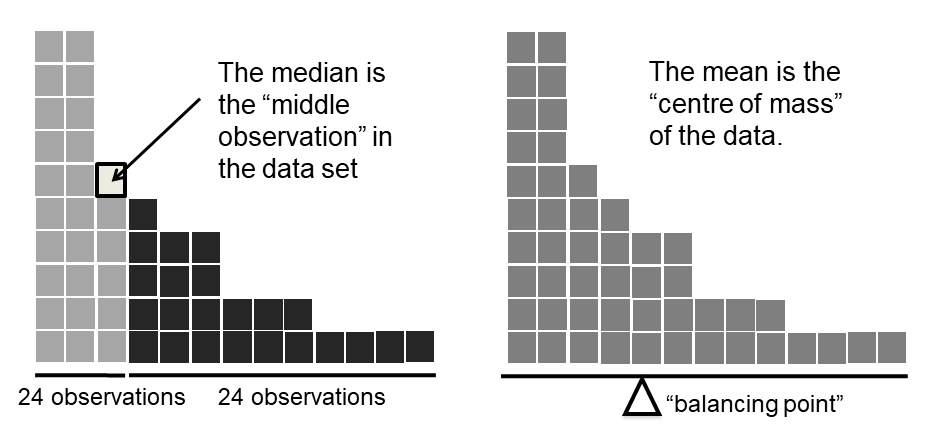
\includegraphics{./img/descriptives2/meanmedian.png}
\caption{\label{fig:meanmedian}An illustration of the difference between how the mean and the median should be interpreted. The mean is basically the ``centre of gravity'' of the data set: if you imagine that the histogram of the data is a solid object, then the point on which you could balance it (as if on a see-saw) is the mean. In contrast, the median is the middle observation. Half of the observations are smaller, and half of the observations are larger.}
\end{figure}

\begin{itemize}
\item
  Knowing how to calculate means and medians is only a part of the story. You also need to understand what each one is saying about the data, and what that implies for when you should use each one. This is illustrated in Figure \ref{fig:meanmedian} the mean is kind of like the ``centre of gravity'' of the data set, whereas the median is the ``middle value'' in the data. What this implies, as far as which one you should use, depends a little on what type of data you've got and what you're trying to achieve. As a rough guide:
\item
  One consequence is that there's systematic differences between the mean and the median when the histogram is asymmetric (skewed; see Section \ref{skewandkurtosis}). This is illustrated in Figure \ref{fig:meanmedian} notice that the median (right hand side) is located closer to the ``body'' of the histogram, whereas the mean (left hand side) gets dragged towards the ``tail'' (where the extreme values are).
\item
  To give a concrete example, suppose Bob (income \$50,000), Kate (income \$60,000) and Jane (income \$65,000) are sitting at a table: the average income at the table is \$58,333 and the median income is \$60,000. Then Bill sits down with them (income \$100,000,000). The average income has now jumped to \$25,043,750 but the median rises only to \$62,500. If you're interested in looking at the overall income at the table, the mean might be the right answer; but if you're interested in what counts as a typical income at the table, the median would be a better choice here.
\end{itemize}

\begin{figure}
\centering
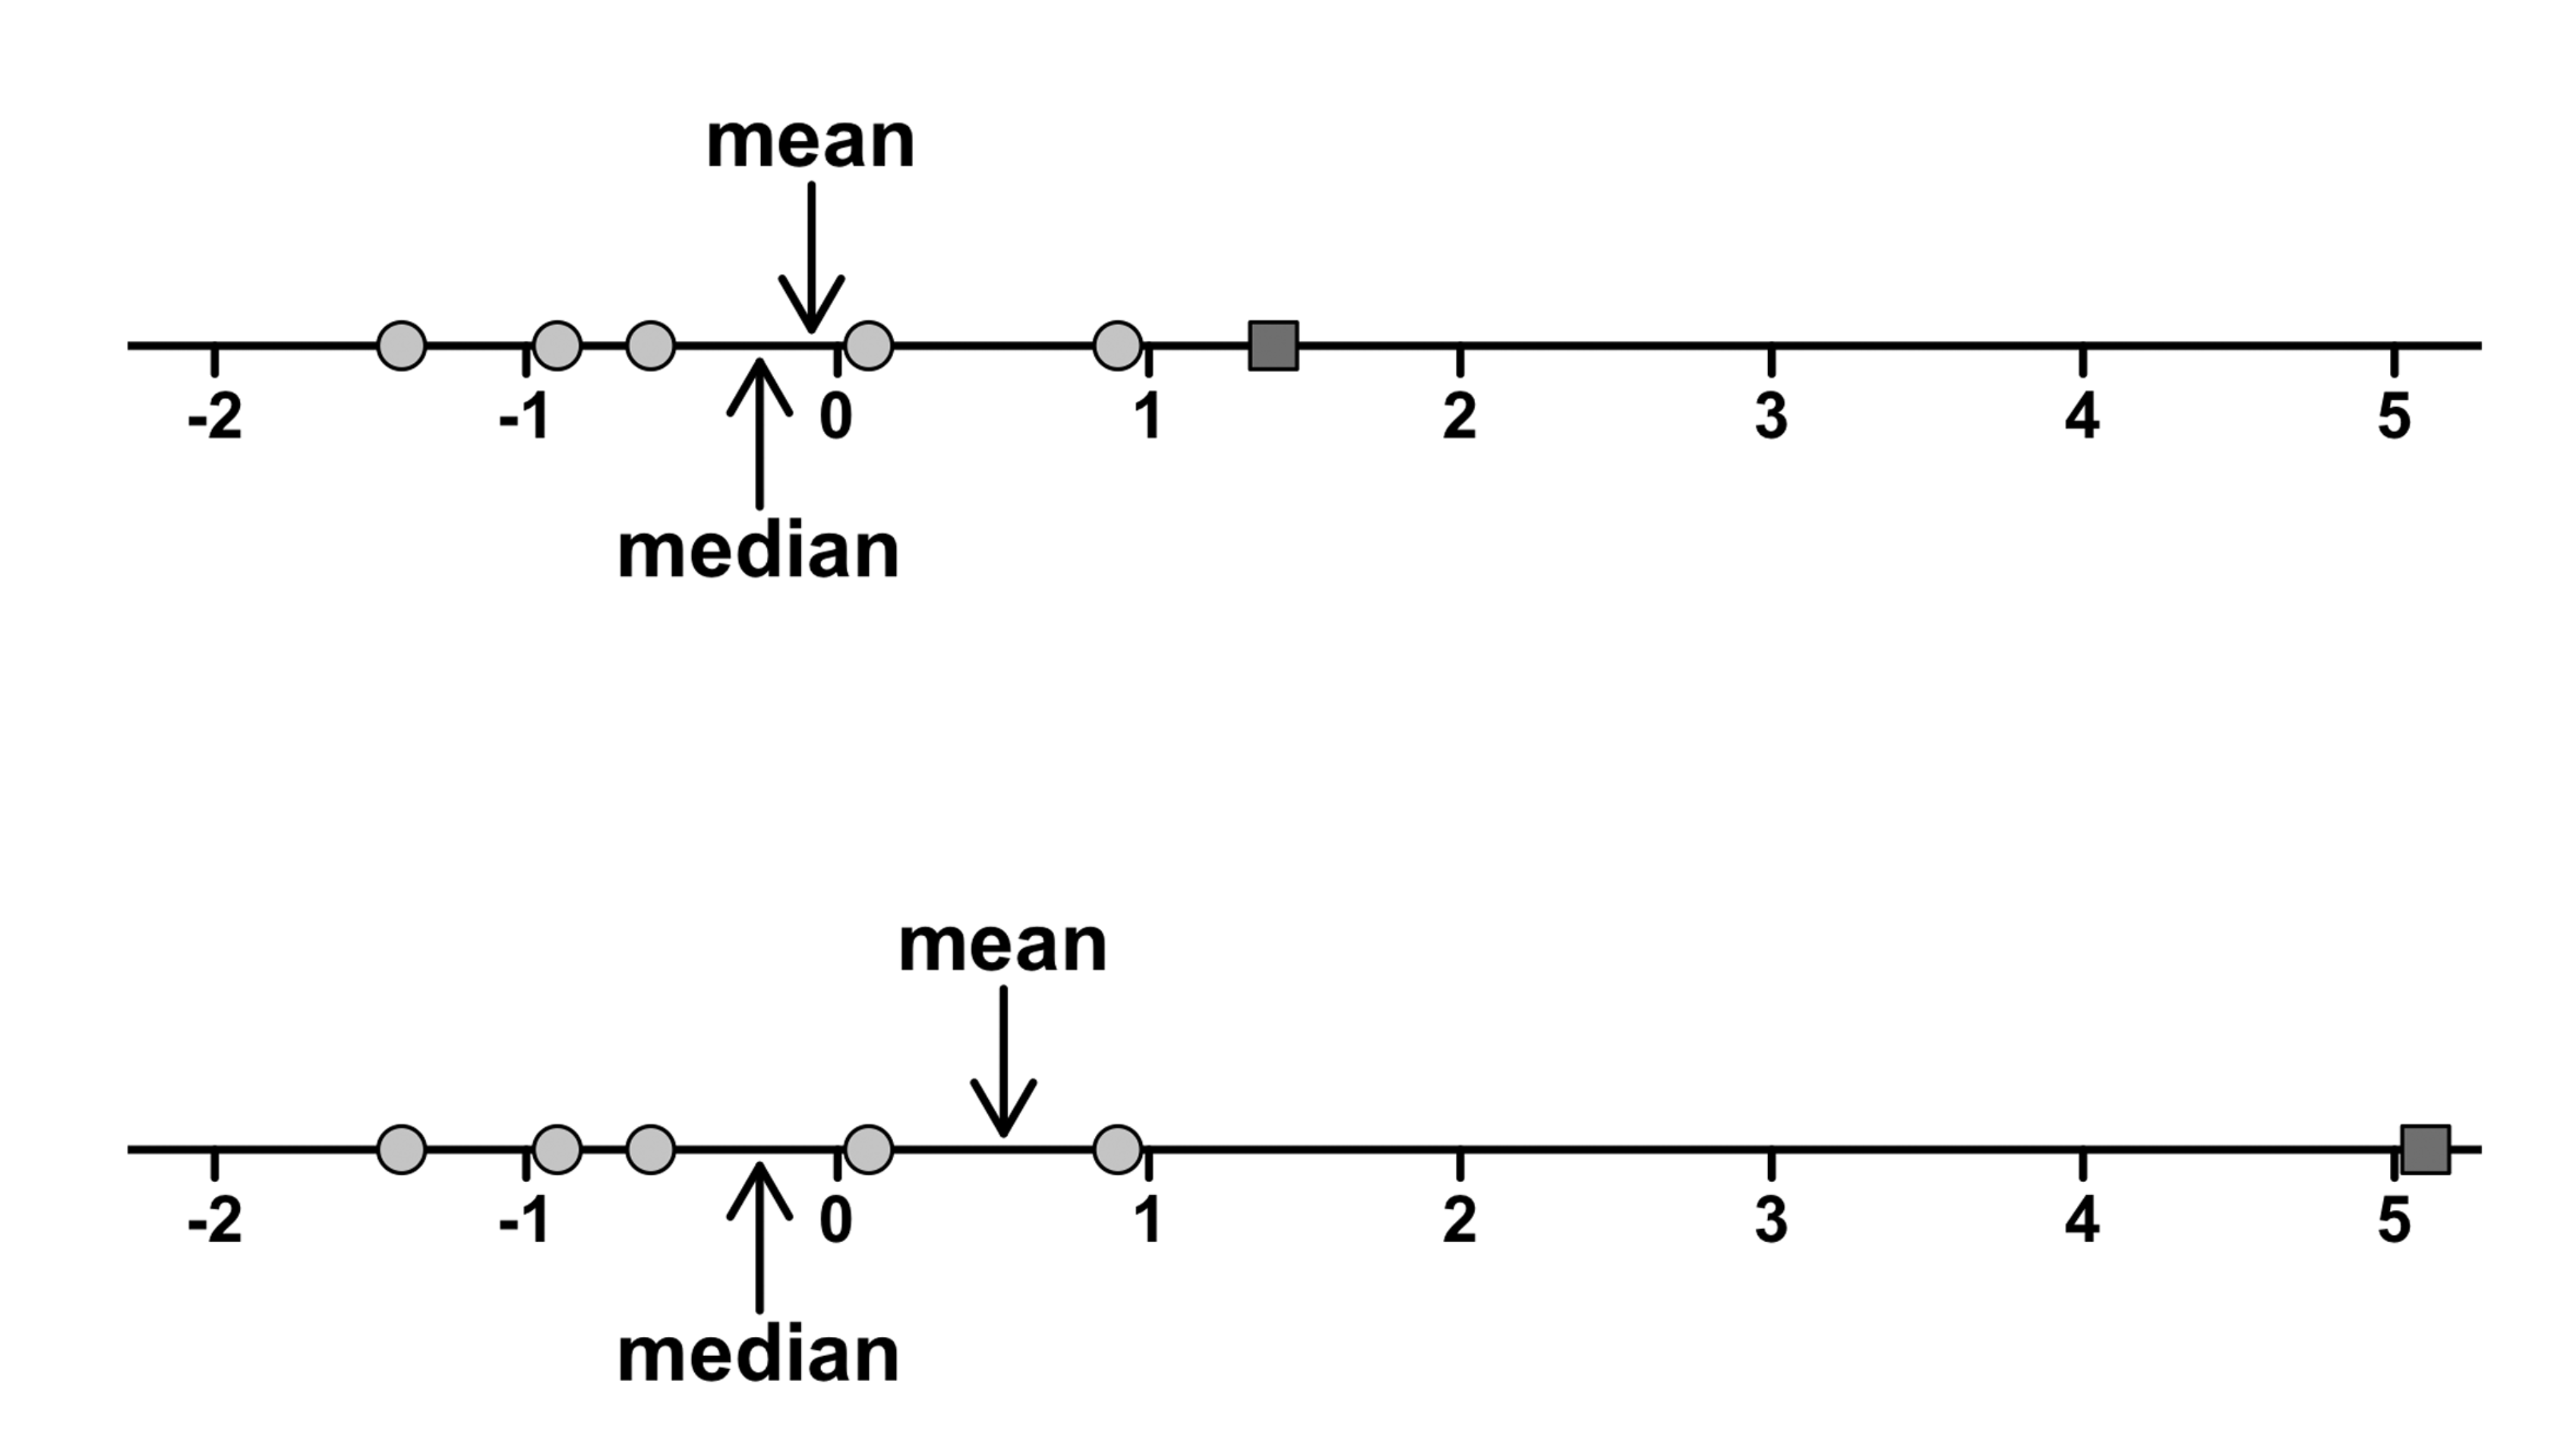
\includegraphics{./img/descriptives2/mean_median.png}
\caption{\label{fig:meanmedian2}Another example of mean and median where mean is moved by the outliers but median is constant.}
\end{figure}

\hypertarget{trimmedmean}{%
\subsection{Trimmed mean}\label{trimmedmean}}

\begin{itemize}
\item
  One of the fundamental rules of applied statistics is that the data are messy. Real life is never simple, and so the data sets that you obtain are never as straightforward as the statistical theory says.\footnote{Or at least, the basic statistical theory -- these days there is a whole subfield of statistics called \emph{robust statistics} that tries to grapple with the messiness of real data and develop theory that can cope with it.} This can have awkward consequences. To illustrate, consider this rather strange looking data set (nevermind what it represents):
  \[
  -100,2,3,4,5,6,7,8,9,10
  \]
\item
  If you were to observe this in a real life data set, you'd probably suspect that something funny was going on with the \(-100\) value. It's probably an \textbf{\emph{outlier}}, a value that doesn't really belong with the others. You might consider removing it from the data set entirely, and in this particular case I'd probably agree with that course of action.
\item
  In real life, however, you don't always get such cut-and-dried examples. For instance, you might get this instead:
  \[
  -15,2,3,4,5,6,7,8,9,12
  \]
\item
  The \(-15\) looks a bit suspicious, but not anywhere near as much as that \(-100\) did. In this case, it's a little trickier. It \emph{might} be a legitimate observation, it might not.
\item
  When faced with a situation where some of the most extreme-valued observations might not be quite trustworthy, the mean is not necessarily a good measure of central tendency. It is highly sensitive to one or two extreme values, and is thus not considered to be a \textbf{\emph{robust}} measure.
\item
  One remedy that we've seen is to use the median. A more general solution is to use a ``trimmed mean''. To calculate a trimmed mean, what you do is ``discard'' the most extreme examples on both ends (i.e., the largest and the smallest), and then take the mean of everything else. The goal is to preserve the best characteristics of the mean and the median:

  \begin{itemize}
  \tightlist
  \item
    just like a median, you aren't highly influenced by extreme outliers, but \ldots{}
  \item
    like the mean, you ``use'' more than one of the observations.
  \end{itemize}
\item
  Generally, we describe a trimmed mean in terms of the percentage of observation on either side that are discarded. So, for instance, a 10\% trimmed mean discards the largest 10\% of the observations \emph{and} the smallest 10\% of the observations, and then takes the mean of the remaining 80\% of the observations.
\item
  Not surprisingly, the 0\% trimmed mean is just the regular mean, and the 50\% trimmed mean is the median. In that sense, trimmed means provide a whole family of central tendency measures that span the range from the mean to the median.
\item
  For our toy example above, we have 10 observations, and so a 10\% trimmed mean is calculated by ignoring the largest value (i.e., \texttt{12}) and the smallest value (i.e., \texttt{-15}) and taking the mean of the remaining values. First, let's enter the data
\end{itemize}

\begin{Shaded}
\begin{Highlighting}[]
\NormalTok{dataset }\OtherTok{\textless{}{-}} \FunctionTok{c}\NormalTok{( }\SpecialCharTok{{-}}\DecValTok{15}\NormalTok{,}\DecValTok{2}\NormalTok{,}\DecValTok{3}\NormalTok{,}\DecValTok{4}\NormalTok{,}\DecValTok{5}\NormalTok{,}\DecValTok{6}\NormalTok{,}\DecValTok{7}\NormalTok{,}\DecValTok{8}\NormalTok{,}\DecValTok{9}\NormalTok{,}\DecValTok{12}\NormalTok{ )}
\end{Highlighting}
\end{Shaded}

Next, let's calculate means and medians:

\begin{Shaded}
\begin{Highlighting}[]
\FunctionTok{mean}\NormalTok{( dataset )}
\end{Highlighting}
\end{Shaded}

\begin{Shaded}
\begin{Highlighting}[]
\NormalTok{\#\# [1] 4.1}
\end{Highlighting}
\end{Shaded}

\begin{Shaded}
\begin{Highlighting}[]
\FunctionTok{median}\NormalTok{( dataset )}
\end{Highlighting}
\end{Shaded}

\begin{Shaded}
\begin{Highlighting}[]
\NormalTok{\#\# [1] 5.5}
\end{Highlighting}
\end{Shaded}

\begin{itemize}
\tightlist
\item
  That's a fairly substantial difference, but I'm tempted to think that the mean is being influenced a bit too much by the extreme values at either end of the data set, especially the \(-15\) one. So let's just try trimming the mean a bit. If I take a 10\% trimmed mean, we'll drop the extreme values on either side, and take the mean of the rest:
\end{itemize}

\begin{Shaded}
\begin{Highlighting}[]
\FunctionTok{mean}\NormalTok{( dataset, }\AttributeTok{trim =}\NormalTok{ .}\DecValTok{1}\NormalTok{)}
\end{Highlighting}
\end{Shaded}

\begin{Shaded}
\begin{Highlighting}[]
\NormalTok{\#\# [1] 5.5}
\end{Highlighting}
\end{Shaded}

\begin{itemize}
\tightlist
\item
  In this case it gives exactly the same answer as the median. Note that, to get a 10\% trimmed mean you write \texttt{trim\ =\ .1}, not \texttt{trim\ =\ 10}.
\end{itemize}

\hypertarget{mode}{%
\subsection{Mode}\label{mode}}

\begin{itemize}
\item
  The \textbf{\emph{mode}} is the last measure of central tendency we'll look at. It is very simple: it is the value that occurs most frequently.
\item
  Let's look at the some soccer data: specifically, the European Cup and Champions League results in the time from 1955-2016.
\item
  Lets find out which team has won the most matches. The command below tells R we just want the first 25 rows of the data.frame.
\end{itemize}

\begin{Shaded}
\begin{Highlighting}[]
\FunctionTok{library}\NormalTok{(engsoccerdata)}

\FunctionTok{table}\NormalTok{(champs}\SpecialCharTok{$}\NormalTok{tiewinner) }\SpecialCharTok{\%\textgreater{}\%} \FunctionTok{sort}\NormalTok{(}\AttributeTok{decreasing=}\NormalTok{T) }\SpecialCharTok{\%\textgreater{}\%}\NormalTok{ .[}\DecValTok{1}\SpecialCharTok{:}\DecValTok{25}\NormalTok{]}
\end{Highlighting}
\end{Shaded}

\begin{Shaded}
\begin{Highlighting}[]
\NormalTok{\#\# }
\NormalTok{\#\#       Real Madrid     Bayern Munich        SL Benfica          AC Milan }
\NormalTok{\#\#               183               134               110               103 }
\NormalTok{\#\#         Barcelona         Liverpool          Juventus       Dinamo Kiev }
\NormalTok{\#\#               101                97                87                82 }
\NormalTok{\#\#            Celtic Manchester United    RSC Anderlecht          AFC Ajax }
\NormalTok{\#\#                81                81                75                71 }
\NormalTok{\#\#    Internazionale  Steaua Bucuresti     Crvena Zvezda           Rangers }
\NormalTok{\#\#                66                63                61                58 }
\NormalTok{\#\# Partizan Belgrade     PSV Eindhoven     Dinamo Zagreb          FC Porto }
\NormalTok{\#\#                52                49                48                46 }
\NormalTok{\#\#   Atletico Madrid     Panathinaikos      BATE Borisov        CSKA Sofia }
\NormalTok{\#\#                45                44                40                40 }
\NormalTok{\#\#       Galatasaray }
\NormalTok{\#\#                40}
\end{Highlighting}
\end{Shaded}

\begin{itemize}
\item
  It appears that the mode of the winning team is `Real Madrid'.
\item
  Of course, the mode is the right (and only) summary for nominal variables.
\item
  But we can compute a mode for all types of variables. For example, let's take a look at the mean, median, and mode of the total number of goals per game.
\end{itemize}

\begin{Shaded}
\begin{Highlighting}[]
\NormalTok{champs }\SpecialCharTok{\%\textless{}\textgreater{}\%} \FunctionTok{mutate}\NormalTok{(}\AttributeTok{total\_goals =}\NormalTok{ hgoal }\SpecialCharTok{+}\NormalTok{ vgoal) }\CommentTok{\# total goals is home team goals + visitor goals}
\end{Highlighting}
\end{Shaded}

\begin{Shaded}
\begin{Highlighting}[]
\FunctionTok{mean}\NormalTok{(champs}\SpecialCharTok{$}\NormalTok{total\_goals)}
\end{Highlighting}
\end{Shaded}

\begin{Shaded}
\begin{Highlighting}[]
\NormalTok{\#\# [1] 2.81642}
\end{Highlighting}
\end{Shaded}

\begin{Shaded}
\begin{Highlighting}[]
\FunctionTok{median}\NormalTok{(champs}\SpecialCharTok{$}\NormalTok{total\_goals)}
\end{Highlighting}
\end{Shaded}

\begin{Shaded}
\begin{Highlighting}[]
\NormalTok{\#\# [1] 3}
\end{Highlighting}
\end{Shaded}

\begin{Shaded}
\begin{Highlighting}[]
\FunctionTok{modeOf}\NormalTok{(champs}\SpecialCharTok{$}\NormalTok{total\_goals)}
\end{Highlighting}
\end{Shaded}

\begin{Shaded}
\begin{Highlighting}[]
\NormalTok{\#\# [1] 2}
\end{Highlighting}
\end{Shaded}

\begin{Shaded}
\begin{Highlighting}[]
\NormalTok{mean\_goals }\OtherTok{\textless{}{-}} \FunctionTok{mean}\NormalTok{(champs}\SpecialCharTok{$}\NormalTok{total\_goals)}
\NormalTok{median\_goals }\OtherTok{\textless{}{-}} \FunctionTok{median}\NormalTok{(champs}\SpecialCharTok{$}\NormalTok{total\_goals)}
\NormalTok{mode\_goals }\OtherTok{\textless{}{-}} \FunctionTok{modeOf}\NormalTok{(champs}\SpecialCharTok{$}\NormalTok{total\_goals)}

\FunctionTok{ggplot}\NormalTok{(champs, }\FunctionTok{aes}\NormalTok{(total\_goals)) }\SpecialCharTok{+} \FunctionTok{geom\_histogram}\NormalTok{(}\AttributeTok{fill=} \StringTok{\textquotesingle{}dimgrey\textquotesingle{}}\NormalTok{) }\SpecialCharTok{+} 
    \FunctionTok{geom\_vline}\NormalTok{(}\AttributeTok{xintercept =}\NormalTok{ mean\_goals, }\AttributeTok{color =} \StringTok{"indianred"}\NormalTok{) }\SpecialCharTok{+} 
    \FunctionTok{geom\_vline}\NormalTok{(}\AttributeTok{xintercept =}\NormalTok{ median\_goals, }\AttributeTok{color =} \StringTok{"steelblue"}\NormalTok{) }\SpecialCharTok{+} 
    \FunctionTok{geom\_vline}\NormalTok{(}\AttributeTok{xintercept =}\NormalTok{ mode\_goals, }\AttributeTok{color =} \StringTok{"yellowgreen"}\NormalTok{) }\SpecialCharTok{+} 
    \FunctionTok{geom\_text}\NormalTok{(}\AttributeTok{data=}\ConstantTok{NULL}\NormalTok{, }\AttributeTok{x =}\NormalTok{ mean\_goals}\FloatTok{{-}.6}\NormalTok{, }\AttributeTok{y=}\DecValTok{1470}\NormalTok{, }\AttributeTok{label =} \StringTok{"mean"}\NormalTok{, }\AttributeTok{color =} \StringTok{"indianred"}\NormalTok{) }\SpecialCharTok{+}
    \FunctionTok{geom\_text}\NormalTok{(}\AttributeTok{data=}\ConstantTok{NULL}\NormalTok{, }\AttributeTok{x =}\NormalTok{ median\_goals}\FloatTok{+.75}\NormalTok{, }\AttributeTok{y=}\DecValTok{1500}\NormalTok{, }\AttributeTok{label =} \StringTok{"median"}\NormalTok{, }\AttributeTok{color =} \StringTok{"steelblue"}\NormalTok{) }\SpecialCharTok{+}
    \FunctionTok{geom\_text}\NormalTok{(}\AttributeTok{data=}\ConstantTok{NULL}\NormalTok{, }\AttributeTok{x =}\NormalTok{ mode\_goals}\FloatTok{{-}.6}\NormalTok{, }\AttributeTok{y=}\DecValTok{1530}\NormalTok{, }\AttributeTok{label =} \StringTok{"mode"}\NormalTok{, }\AttributeTok{color =} \StringTok{"yellowgreen"}\NormalTok{)}
\end{Highlighting}
\end{Shaded}

\begin{verbatim}
## `stat_bin()` using `bins = 30`. Pick better value with `binwidth`.
\end{verbatim}

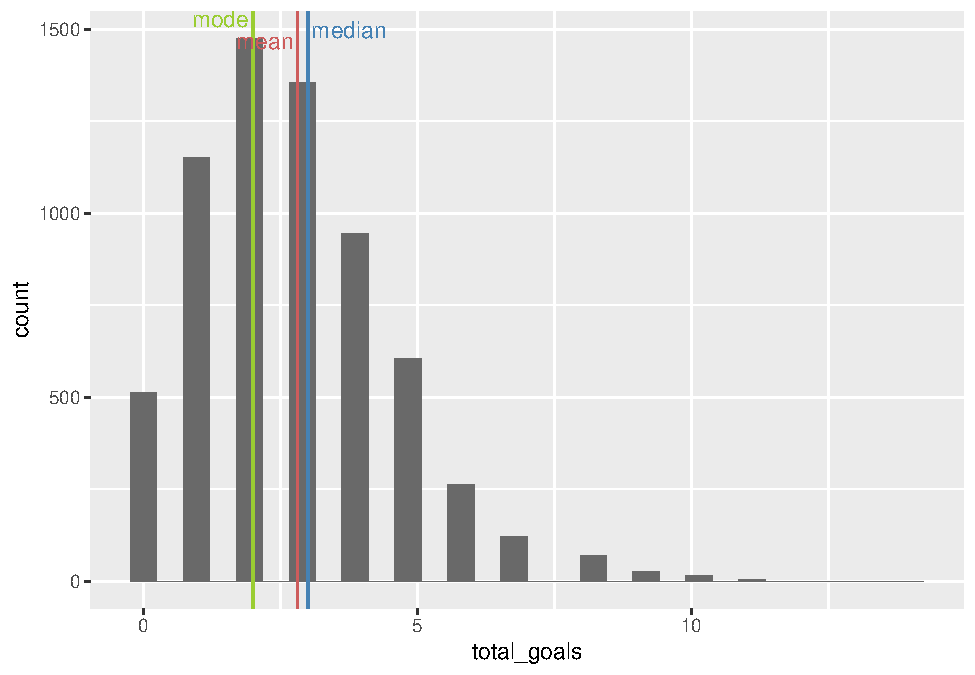
\includegraphics{main_files/figure-latex/unnamed-chunk-175-1.pdf}

\hypertarget{summary}{%
\subsection{Summary}\label{summary}}

\begin{itemize}
\tightlist
\item
  There are multiple measures of central tendency that can be used to summarize an aspect of a distribution: \textbf{\_ (arithmetic) mean, median, and mode\_}.
\item
  They answer different questions about distribution. For example, in the distribution of number of goals per game in the previous section

  \begin{itemize}
  \tightlist
  \item
    mean: ``If the same number of goals were scored in each game, how many goals would be scored?''
  \item
    median: ``What is a `mediocre' game like?''
  \item
    mode: ``What is the most typical game like?''
  \end{itemize}
\end{itemize}

\hypertarget{var}{%
\section{Measures of variability}\label{var}}

\begin{itemize}
\tightlist
\item
  The statistics that we've discussed so far all relate to \emph{central tendency}. That is, they all talk about which values are ``in the middle'' or ``popular'' in the data.
\item
  The second thing that we really want is a measure of the \textbf{\emph{variability}} of the data.

  \begin{itemize}
  \tightlist
  \item
    That is, how ``spread out'' are the data?
  \item
    In other words, how `representative' is our measure of central tendency of most data points.
  \end{itemize}
\item
  Let's consider interval and ratio scale data.
\end{itemize}

\hypertarget{range}{%
\subsection{Range}\label{range}}

\begin{itemize}
\tightlist
\item
  The \textbf{\emph{range}} of a variable is very simple: it's the biggest value minus the smallest value. For the sleep data, the maximum value is 20, and the minimum value is 2. We can calculate these values in R using the \texttt{max()} and \texttt{min()} functions:
\end{itemize}

\begin{Shaded}
\begin{Highlighting}[]
\FunctionTok{max}\NormalTok{( mammalian\_sleep}\SpecialCharTok{$}\NormalTok{sleep\_total\_h )}
\end{Highlighting}
\end{Shaded}

\begin{Shaded}
\begin{Highlighting}[]
\NormalTok{\#\# [1] 20}
\end{Highlighting}
\end{Shaded}

\begin{Shaded}
\begin{Highlighting}[]
\FunctionTok{min}\NormalTok{( mammalian\_sleep}\SpecialCharTok{$}\NormalTok{sleep\_total\_h )}
\end{Highlighting}
\end{Shaded}

\begin{Shaded}
\begin{Highlighting}[]
\NormalTok{\#\# [1] 2}
\end{Highlighting}
\end{Shaded}

where I've omitted the output because it's not interesting.

\begin{itemize}
\tightlist
\item
  The other possibility is to use the \texttt{range()} function; which outputs both the minimum value and the maximum value in a vector, like this:
\end{itemize}

\begin{Shaded}
\begin{Highlighting}[]
\FunctionTok{range}\NormalTok{( mammalian\_sleep}\SpecialCharTok{$}\NormalTok{sleep\_total\_h )}
\end{Highlighting}
\end{Shaded}

\begin{Shaded}
\begin{Highlighting}[]
\NormalTok{\#\# [1]  2 20}
\end{Highlighting}
\end{Shaded}

\begin{itemize}
\tightlist
\item
  Although the range is the simplest way to quantify the notion of ``variability'', it's one of the worst. Recall from our discussion of the mean that we want our summary measure to be robust. If the data set has one or two extremely bad values in it, we'd like our statistics not to be unduly influenced by these cases. If we look once again at our toy example of a data set containing very extreme outliers\ldots{}
  \[
  -100,2,3,4,5,6,7,8,9,10
  \]
  \ldots{} it is clear that the range is not robust, since this has a range of 110, but if the outlier were removed we would have a range of only 8.
\end{itemize}

\hypertarget{quantiles-and-percentile}{%
\subsection{Quantiles and percentile}\label{quantiles-and-percentile}}

\begin{itemize}
\item
  A key concept we will need to build on to conceptualize several other measures of variability are \textbf{\emph{quantiles}} or \textbf{\emph{percentiles}}.
\item
  A \textbf{\emph{percentile}} is the smallest value in a dataset such that a set percentage is smaller than it. (A \textbf{\emph{quantile}} does pretty much the same but is more generic.)
\item
  For example, if the 10-th percentile (i.e., the \(0.1\) quantile) of a list of values is 73, this means that 10 percent of the values are smaller than or equal to 73.
\item
  Let's take a look at the 20 shortest sorted sleep durations and determine the 10-th percentile (\(0.1\) quantile), 30-th percentile (\(0.3\) quantile), 50-th percentile (\(0.5\) quantile), and the 90-th percentile (\(0.9\) quantile).
\item
  Here are the values:
\end{itemize}

\begin{Shaded}
\begin{Highlighting}[]
\FunctionTok{sort}\NormalTok{(mammalian\_sleep}\SpecialCharTok{$}\NormalTok{sleep\_total\_h)[}\DecValTok{1}\SpecialCharTok{:}\DecValTok{20}\NormalTok{]}
\end{Highlighting}
\end{Shaded}

\begin{Shaded}
\begin{Highlighting}[]
\NormalTok{\#\#  [1] 2 3 3 3 3 3 4 4 4 4 4 5 5 5 5 6 6 6 6 7}
\end{Highlighting}
\end{Shaded}

\begin{itemize}
\tightlist
\item
  And here is a sorted plot of the 20 smallest values:
\end{itemize}

\begin{Shaded}
\begin{Highlighting}[]
\NormalTok{quantile }\OtherTok{\textless{}{-}} \FunctionTok{c}\NormalTok{(}\FloatTok{0.1}\NormalTok{,}\FloatTok{0.3}\NormalTok{,}\FloatTok{0.5}\NormalTok{,}\FloatTok{0.9}\NormalTok{)}
\NormalTok{quantile\_points }\OtherTok{\textless{}{-}} \FunctionTok{c}\NormalTok{(}\FloatTok{0.1}\NormalTok{,}\FloatTok{0.3}\NormalTok{,}\FloatTok{0.5}\NormalTok{,}\FloatTok{0.9}\NormalTok{)}\SpecialCharTok{*}\DecValTok{20}
\NormalTok{quantile\_labels }\OtherTok{\textless{}{-}} \FunctionTok{sprintf}\NormalTok{(}\StringTok{"\%0.1f quantile}\SpecialCharTok{\textbackslash{}n}\StringTok{(point \%d of 20)"}\NormalTok{, quantile, quantile\_points)}
\FunctionTok{ggplot}\NormalTok{(}\AttributeTok{data=}\ConstantTok{NULL}\NormalTok{, }\FunctionTok{aes}\NormalTok{(}\AttributeTok{x=}\DecValTok{1}\SpecialCharTok{:}\DecValTok{20}\NormalTok{, }\AttributeTok{y=}\FunctionTok{sort}\NormalTok{(mammalian\_sleep}\SpecialCharTok{$}\NormalTok{sleep\_total\_h)[}\DecValTok{1}\SpecialCharTok{:}\DecValTok{20}\NormalTok{])) }\SpecialCharTok{+}
    \FunctionTok{geom\_point}\NormalTok{() }\SpecialCharTok{+}
    \FunctionTok{geom\_vline}\NormalTok{(}\AttributeTok{xintercept =}\NormalTok{ quantile\_points) }\SpecialCharTok{+}
    \FunctionTok{geom\_label}\NormalTok{(}\FunctionTok{aes}\NormalTok{(}\AttributeTok{x=}\NormalTok{quantile\_points, }\AttributeTok{y=}\FloatTok{6.5}\NormalTok{, }\AttributeTok{label=}\NormalTok{quantile\_labels )) }\SpecialCharTok{+}
    \FunctionTok{scale\_x\_continuous}\NormalTok{(}\AttributeTok{breaks =} \DecValTok{1}\SpecialCharTok{:}\DecValTok{20}\NormalTok{) }\SpecialCharTok{+} \FunctionTok{xlab}\NormalTok{(}\StringTok{"Position in ordered vector"}\NormalTok{) }\SpecialCharTok{+} \FunctionTok{ylab}\NormalTok{(}\StringTok{"Sleep (hours)"}\NormalTok{)}
\end{Highlighting}
\end{Shaded}

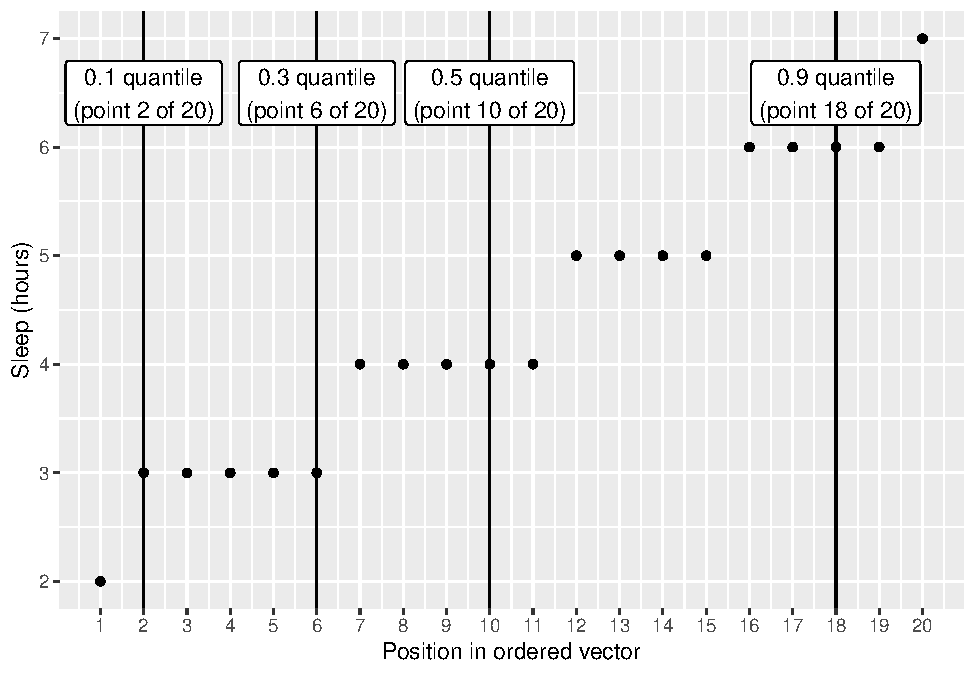
\includegraphics{main_files/figure-latex/unnamed-chunk-179-1.pdf}

\begin{itemize}
\tightlist
\item
  As you can see:

  \begin{itemize}
  \tightlist
  \item
    10-th percentile (\(0.1\) quantile): 3 {[}to be found at position 2, since 2 data points constitute 10 percent of the data{]}
  \item
    30-th percentile (\(0.3\) quantile): 3 {[}to be found at position 6, since 6 data points constitute 30 percent of the data{]}
  \item
    50-th percentile (\(0.5\) quantile): 4 {[}to be found at position 10, since 10 data points constitute 50 percent of the data{]}
  \item
    90-th percentile (\(0.9\) quantile): 6 {[}to be found at position 18, since 18 data points constitute 90 percent of the data{]}
  \end{itemize}
\item
  The 50-th percentile is the median.
\end{itemize}

\hypertarget{interquartile-range}{%
\subsection{Interquartile range}\label{interquartile-range}}

\begin{itemize}
\tightlist
\item
  The \textbf{\emph{interquartile range}} (IQR) is like the range, but instead of calculating the difference between the biggest and smallest value, it calculates the difference between the 25th quantile and the 75th quantile.
\item
  R provides you with a way of calculating quantiles, using the (surprise, surprise) \texttt{quantile()} function. Let's use it to calculate the median sleep durations:
\end{itemize}

\begin{Shaded}
\begin{Highlighting}[]
\FunctionTok{quantile}\NormalTok{( }\AttributeTok{x =}\NormalTok{ mammalian\_sleep}\SpecialCharTok{$}\NormalTok{sleep\_total\_h, }\AttributeTok{probs =}\NormalTok{ .}\DecValTok{5}\NormalTok{)}
\end{Highlighting}
\end{Shaded}

\begin{Shaded}
\begin{Highlighting}[]
\NormalTok{\#\# 50\% }
\NormalTok{\#\#  10}
\end{Highlighting}
\end{Shaded}

\begin{itemize}
\tightlist
\item
  And not surprisingly, this agrees with the answer that we saw earlier with the \texttt{median()} function. Now, we can actually input lots of quantiles at once, by specifying a vector for the \texttt{probs} argument. So lets do that, and get the 25th and 75th percentile:
\end{itemize}

\begin{Shaded}
\begin{Highlighting}[]
\FunctionTok{quantile}\NormalTok{( }\AttributeTok{x =}\NormalTok{ mammalian\_sleep}\SpecialCharTok{$}\NormalTok{sleep\_total\_h, }\AttributeTok{probs =} \FunctionTok{c}\NormalTok{(.}\DecValTok{25}\NormalTok{,.}\DecValTok{75}\NormalTok{) )}
\end{Highlighting}
\end{Shaded}

\begin{Shaded}
\begin{Highlighting}[]
\NormalTok{\#\# 25\% 75\% }
\NormalTok{\#\#   8  14}
\end{Highlighting}
\end{Shaded}

\begin{itemize}
\tightlist
\item
  And, by noting that \(14 - 8 = 6\), we can see that the interquartile range for the sleep durations is 6. Of course, that seems like too much work to do all that typing, so R has a built in function called \texttt{IQR()} that we can use:
\end{itemize}

\begin{Shaded}
\begin{Highlighting}[]
\FunctionTok{IQR}\NormalTok{( }\AttributeTok{x =}\NormalTok{ mammalian\_sleep}\SpecialCharTok{$}\NormalTok{sleep\_total\_h )}
\end{Highlighting}
\end{Shaded}

\begin{Shaded}
\begin{Highlighting}[]
\NormalTok{\#\# [1] 6}
\end{Highlighting}
\end{Shaded}

\begin{itemize}
\item
  While it's obvious how to interpret the range, it's a little less obvious how to interpret the IQR. The simplest way to think about it is like this: the interquartile range is the range spanned by the ``middle half'' of the data. That is, one quarter of the data falls below the 25th percentile, one quarter of the data is above the 75th percentile, leaving the ``middle half'' of the data lying in between the two. And the IQR is the range covered by that middle half.
\item
  IQR is used to identify the outliers (i.e.~extreme values). Any value above \texttt{Q3\ +\ IQR\ *1.5} or below \texttt{Q1\ -\ IQR*1.5} is considered to be an outlier.
\end{itemize}

\hypertarget{aad}{%
\subsection{Mean absolute deviation}\label{aad}}

\begin{itemize}
\item
  The range and the interquartile range, both rely on the idea that we can measure the spread of the data by looking at the quantiles of the data.
\item
  However, this isn't the only way to think about the problem. A different approach is to select a meaningful reference point (usually the mean or the median) and then report the \textbf{\emph{``typical'' deviations}} from that reference point.
\item
  Let's go through the \textbf{\emph{mean absolute deviation}} (AAD for average absolute deviation, since MAD is reserved for the median absolute deviation) from the mean a little more slowly. One useful thing about this measure is that the name actually tells you exactly how to calculate it:
  \[
  AAD(X) = \frac{1}{N} \sum_{i = 1}^N |X_i - \bar{X}|
  \]
\item
  Let's compute the AAD for the first data points in the sleep data:
  \[
  12, 17, 14, 15, 4
  \]
\item
  The mean of the dataset is 12.4. That is, \(\bar{X} = 12.4\)
\item
  The deviations \(X_i - \bar{X}\) are:
  \[
  -0.4, 4.6, 1.6, 2.6, -8.4
  \]
\item
  The absolute deviations \(|X_i - \bar{X}|\) are:
  \[
  0.4, 4.6, 1.6, 2.6, 8.4
  \]
\item
  The sum of the absolute deviations \(\sum_{i = 1}^N |X_i - \bar{X}|\) is 17.6.
\item
  And \(N=5\), which means, that, in our case: \(AAD(X) = \frac{1}{N} \sum_{i = 1}^N |X_i - \bar{X}| = 3.52\)
\item
  In R, we can compute it for the entire vector.
\end{itemize}

\begin{Shaded}
\begin{Highlighting}[]
\NormalTok{mean\_sleep }\OtherTok{\textless{}{-}} \FunctionTok{mean}\NormalTok{(mammalian\_sleep}\SpecialCharTok{$}\NormalTok{sleep\_total\_h)}
\NormalTok{deviation\_sleep }\OtherTok{\textless{}{-}}\NormalTok{ mean\_sleep }\SpecialCharTok{{-}}\NormalTok{ mammalian\_sleep}\SpecialCharTok{$}\NormalTok{sleep\_total\_h}
\FunctionTok{mean}\NormalTok{( }\FunctionTok{abs}\NormalTok{(deviation\_sleep) )}
\end{Highlighting}
\end{Shaded}

\begin{Shaded}
\begin{Highlighting}[]
\NormalTok{\#\# [1] 3.576717}
\end{Highlighting}
\end{Shaded}

\begin{itemize}
\tightlist
\item
  An alternative, more compact way to write it is using (lots) pipes:
\end{itemize}

\begin{Shaded}
\begin{Highlighting}[]
\NormalTok{mammalian\_sleep}\SpecialCharTok{$}\NormalTok{sleep\_total\_h }\SpecialCharTok{\%\textgreater{}\%} \FunctionTok{subtract}\NormalTok{(., }\FunctionTok{mean}\NormalTok{(.)) }\SpecialCharTok{\%\textgreater{}\%} \FunctionTok{abs}\NormalTok{() }\SpecialCharTok{\%\textgreater{}\%} \FunctionTok{mean}\NormalTok{()}
\end{Highlighting}
\end{Shaded}

\begin{Shaded}
\begin{Highlighting}[]
\NormalTok{\#\# [1] 3.576717}
\end{Highlighting}
\end{Shaded}

\begin{itemize}
\tightlist
\item
  The interpretation of the AAD is quite straightforward: It is the average distance from the average. When it's big, the values are quite spread out. When it's small, they are close. The units are the same (hours in our case).
\end{itemize}

\hypertarget{variance}{%
\subsection{Variance}\label{variance}}

\begin{itemize}
\item
  Although the mean absolute deviation measure has its uses, it's not the best measure of variability to use.
\item
  For a number of practical reasons, there are some solid reasons to prefer squared deviations rather than absolute deviations. A measure of variability based on \emph{squared deviations} has a number of useful properties in \emph{inferential statistics} and \emph{statistical modeling}.\footnote{I will very briefly mention the one that I think is coolest, for a very particular definition of ``cool'', that is. Variances are \emph{additive}. Here's what that means: suppose I have two variables \(X\) and \(Y\), whose variances are \(\mbox{Var}(X)\) and \(\mbox{Var}(Y)\) respectively. Now imagine I want to define a new variable \(Z\) that is the sum of the two, \(Z = X+Y\). As it turns out, the variance of \(Z\) is equal to \(\mbox{Var}(X) + \mbox{Var}(Y)\). This is a \emph{very} useful property, but it's not true of the other measures that I talk about in this section.}
\item
  If we do that, we obtain a measure is called the \textbf{\emph{variance}}, which for a specific set of observations \(X\) is written \(\mbox{s}_X^2\). It is the most wide-spread measure of variability because it is a key concept in \emph{inferential statistics}.
\item
  The formula that we use to calculate the variance of a set of observations is as follows:
  \[
  \mbox{s}_X^2 = \frac{1}{N-1} \sum_{i=1}^N \left( X_i - \bar{X} \right)^2
  \]
\item
  As you can see, it's basically the same formula that we used to calculate the mean absolute deviation, except that:

  \begin{enumerate}
  \def\labelenumi{\arabic{enumi}.}
  \tightlist
  \item
    Instead of using ``absolute deviations'' we use ``squared deviations''.
  \item
    Instead of dividing by \(N\) (which gives us the average deviation), we divide by \(N-1\) (which gives us \emph{`sort-of-the-average'}). {[}We will talk about this in a little while.{]}
  \end{enumerate}
\end{itemize}

\begin{itemize}
\tightlist
\item
  Now that we've got the basic idea, let's have a look at a concrete example. Once again, let's use the first five sleep durations. If we follow the same approach that we took last time, we end up with the following table:
\end{itemize}

\begin{table}

\caption{\label{tab:unnamed-chunk-188}Regular, abssolute, and squared deviations}
\centering
\begin{tabular}[t]{lllll}
\toprule
Notation [English] & \$i\$ [animal] & \$X\_i\$ [value] & \$X\_i - \textbackslash{}bar\{X\}\$ [deviation from mean] & \$(X\_i - \textbackslash{}bar\{X\})\textasciicircum{}2\$ [squared deviation]\\
\midrule
 & 1 & 12 & -0.4 & 0.16\\
 & 2 & 17 & 4.6 & 21.16\\
 & 3 & 14 & 1.6 & 2.56\\
 & 4 & 15 & 2.6 & 6.76\\
 & 5 & 4 & -8.4 & 70.56\\
\bottomrule
\end{tabular}
\end{table}

\begin{itemize}
\tightlist
\item
  That last column contains all of our squared deviations, so all we have to do is average them. If we do that by typing all the numbers into R by hand\ldots{}
\end{itemize}

\begin{Shaded}
\begin{Highlighting}[]
\NormalTok{( }\FloatTok{0.16+21.16+2.56+6.76+70.56}\NormalTok{ ) }\SpecialCharTok{/}\NormalTok{ (}\DecValTok{5{-}1}\NormalTok{)}
\end{Highlighting}
\end{Shaded}

\begin{Shaded}
\begin{Highlighting}[]
\NormalTok{\#\# [1] 25.3}
\end{Highlighting}
\end{Shaded}

\begin{itemize}
\item
  We end up with a variance of 25.3. Exciting, isn't it? For the moment, let's ignore the burning question that you're all probably thinking (i.e., what the heck does a variance of 25.3 actually mean?) and instead talk a bit more about how to do the calculations in R.
\item
  As always, we want to avoid having to type in a whole lot of numbers ourselves. And as it happens, we have the vector \texttt{X} lying around, which we created in the previous section. With this in mind, we can calculate the variance of \texttt{X} by using the following command,
\end{itemize}

\begin{Shaded}
\begin{Highlighting}[]
\NormalTok{X }\OtherTok{\textless{}{-}}\NormalTok{ mammalian\_sleep}\SpecialCharTok{$}\NormalTok{sleep\_total\_h[}\DecValTok{1}\SpecialCharTok{:}\DecValTok{5}\NormalTok{]}
\NormalTok{(X }\SpecialCharTok{{-}} \FunctionTok{mean}\NormalTok{(X) )}\SpecialCharTok{\^{}}\DecValTok{2} \SpecialCharTok{/}\NormalTok{ (}\FunctionTok{length}\NormalTok{(X) }\SpecialCharTok{{-}} \DecValTok{1}\NormalTok{)}
\end{Highlighting}
\end{Shaded}

\begin{Shaded}
\begin{Highlighting}[]
\NormalTok{\#\# [1]  0.04  5.29  0.64  1.69 17.64}
\end{Highlighting}
\end{Shaded}

and as usual we get the same answer as the one that we got when we did everything by hand. However, I \emph{still} think that this is too much typing. Fortunately, R has a built in function called \texttt{var()} which does calculate variances. So we could also do this\ldots{}

\begin{Shaded}
\begin{Highlighting}[]
\FunctionTok{var}\NormalTok{(X)}
\end{Highlighting}
\end{Shaded}

\begin{Shaded}
\begin{Highlighting}[]
\NormalTok{\#\# [1] 25.3}
\end{Highlighting}
\end{Shaded}

and you get the same answer. Great.

\hypertarget{sd}{%
\subsection{Standard deviation}\label{sd}}

\begin{itemize}
\item
  One problem with the variance is that it is expressed in odd units. In the case above it's \(h^2\) (\emph{hours squared}). I know what \(m^2\) is, but what are \(h^2\)? No idea.
\item
  Suppose that you'd like to have a measure that is expressed in the same units as the data itself (i.e., points, not points-squared). What should you do?
\item
  The solution to the problem is obvious: take the square root of the variance, known as the \textbf{\emph{standard deviation}}, also called the ``root mean squared deviation'', or RMSD. This solves out problem fairly neatly.
\item
  While nobody has a clue what \emph{``a variance of 19.95 hours-squared''} really means, it's much easier to understand \emph{``a standard deviation of 4.5 hours''}, since it's expressed in the original units.
\item
  It is traditional to refer to the standard deviation of a sample of data as \(s_x\), though ``sd'' and ``std dev.'' are also used at times. Because the standard deviation is equal to the square root of the variance, you probably won't be surprised to see that the formula is:
  \[
  s_x = \sqrt{ \frac{1}{N-1} \sum_{i=1}^N \left( X_i - \bar{X} \right)^2 }
  \]
\item
  Interpreting standard deviations is slightly more complex. Because the standard deviation is derived from the variance, and the variance is a quantity that has little to no meaning that makes sense to us humans, the standard deviation doesn't have a simple interpretation.
\item
  As a consequence, most of us just rely on a \textbf{simple rule of thumb}: \textbf{``in general, you should expect 68\% of the data to fall within 1 standard deviation of the mean, 95\% of the data to fall within 2 standard deviation of the mean, and 99.7\% of the data to fall within 3 standard deviations of the mean''}. This rule tends to work pretty well most of the time, but it's not exact: it's actually calculated based on an \emph{assumption} that the histogram is symmetric and ``bell shaped''. (Strictly, the assumption is that the data are \emph{normally} distributed, which is an important concept that we'll discuss more later).
\end{itemize}

\begin{Shaded}
\begin{Highlighting}[]
\NormalTok{  p }\OtherTok{\textless{}{-}}\NormalTok{ mammalian\_sleep }\SpecialCharTok{\%\textgreater{}\%}
        \FunctionTok{ggplot}\NormalTok{(}\FunctionTok{aes}\NormalTok{(sleep\_total\_h)) }\SpecialCharTok{+}
        \FunctionTok{geom\_histogram}\NormalTok{(}\AttributeTok{binwidth =} \DecValTok{1}\NormalTok{,}
                       \AttributeTok{color =} \StringTok{"black"}\NormalTok{,}
                       \AttributeTok{fill =} \StringTok{"lightgrey"}\NormalTok{)}

\NormalTok{  sleep\_sd }\OtherTok{\textless{}{-}} \FunctionTok{sd}\NormalTok{(mammalian\_sleep}\SpecialCharTok{$}\NormalTok{sleep\_total\_h)}
\NormalTok{  sleep\_mean }\OtherTok{\textless{}{-}} \FunctionTok{mean}\NormalTok{(mammalian\_sleep}\SpecialCharTok{$}\NormalTok{sleep\_total\_h)}
\NormalTok{  bars }\OtherTok{\textless{}{-}} \FunctionTok{c}\NormalTok{(sleep\_mean}\SpecialCharTok{{-}}\NormalTok{sleep\_sd, sleep\_mean, sleep\_mean}\SpecialCharTok{+}\NormalTok{sleep\_sd)}
\NormalTok{  bar\_labels }\OtherTok{\textless{}{-}} \FunctionTok{c}\NormalTok{(}\StringTok{"mean{-}1*sd"}\NormalTok{, }\StringTok{"mean"}\NormalTok{, }\StringTok{"mean+1*sd"}\NormalTok{)}
\NormalTok{  p }\OtherTok{\textless{}{-}}\NormalTok{ p }\SpecialCharTok{+} \FunctionTok{geom\_vline}\NormalTok{(}\AttributeTok{xintercept =}\NormalTok{ bars, }\AttributeTok{color =} \StringTok{"red"}\NormalTok{) }\SpecialCharTok{+}
      \FunctionTok{geom\_label}\NormalTok{(}\AttributeTok{data=}\ConstantTok{NULL}\NormalTok{, }\FunctionTok{aes}\NormalTok{(}\AttributeTok{x=}\NormalTok{bars[}\DecValTok{1}\NormalTok{], }\AttributeTok{y=} \DecValTok{10}\NormalTok{, }\AttributeTok{label =}\NormalTok{ bar\_labels[}\DecValTok{1}\NormalTok{])) }\SpecialCharTok{+}
      \FunctionTok{geom\_label}\NormalTok{(}\AttributeTok{data=}\ConstantTok{NULL}\NormalTok{, }\FunctionTok{aes}\NormalTok{(}\AttributeTok{x=}\NormalTok{bars[}\DecValTok{2}\NormalTok{], }\AttributeTok{y=} \DecValTok{10}\NormalTok{, }\AttributeTok{label =}\NormalTok{ bar\_labels[}\DecValTok{2}\NormalTok{])) }\SpecialCharTok{+}
      \FunctionTok{geom\_label}\NormalTok{(}\AttributeTok{data=}\ConstantTok{NULL}\NormalTok{, }\FunctionTok{aes}\NormalTok{(}\AttributeTok{x=}\NormalTok{bars[}\DecValTok{3}\NormalTok{], }\AttributeTok{y=} \DecValTok{10}\NormalTok{, }\AttributeTok{label =}\NormalTok{ bar\_labels[}\DecValTok{3}\NormalTok{]))}
\NormalTok{  p}
\end{Highlighting}
\end{Shaded}

\begin{figure}
\centering
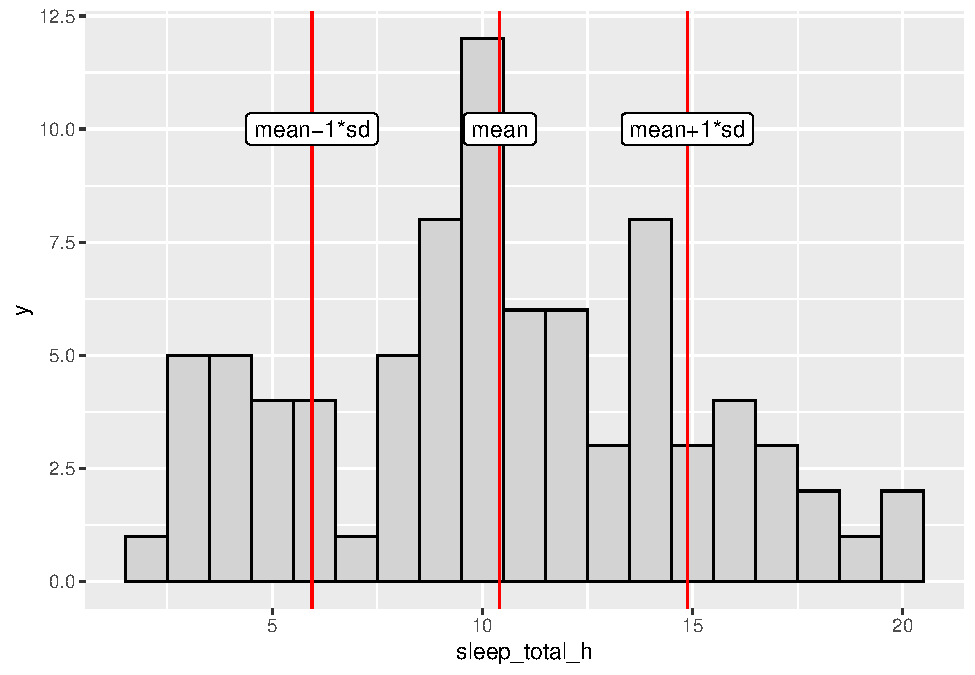
\includegraphics{main_files/figure-latex/aflsd-1.pdf}
\caption{\label{fig:aflsd}An illustration of the standard deviation.}
\end{figure}

\begin{Shaded}
\begin{Highlighting}[]
  \FunctionTok{with}\NormalTok{(mammalian\_sleep, }\FunctionTok{mean}\NormalTok{(sleep\_total\_h}\SpecialCharTok{\textgreater{}}\NormalTok{(sleep\_mean}\SpecialCharTok{{-}}\NormalTok{sleep\_sd) }\SpecialCharTok{\&}\NormalTok{ sleep\_total\_h}\SpecialCharTok{\textless{}}\NormalTok{(sleep\_mean}\SpecialCharTok{+}\NormalTok{sleep\_sd) ))}
\end{Highlighting}
\end{Shaded}

\begin{Shaded}
\begin{Highlighting}[]
\NormalTok{\#\# [1] 0.6385542}
\end{Highlighting}
\end{Shaded}

\hypertarget{bessels-correction-whats-up-with-all-those-n-1s-in-the-denominator}{%
\subsubsection{\texorpdfstring{Bessel's correction: What's up with all those \(N-1\)s in the denominator?}{Bessel's correction: What's up with all those N-1s in the denominator?}}\label{bessels-correction-whats-up-with-all-those-n-1s-in-the-denominator}}

\begin{itemize}
\item
  Now, what's going on with that \(N-1\), and why do I still call the sample variance a \emph{`sort-of-the-average'} of the squared deviations? Let's address these questions in turn.
\item
  The important thing to note about variance and standard deviation is they serve \emph{two} purposes: They are used to (i) describe a \textbf{sample}, but also to (ii) tentatively characterize the larger population from which the sample is.
\item
  You are \emph{usually} not really interested in the variance of a particular set of numbers, but rather in what they represent. So function number (ii) is the far more dominant use.
\item
  In our case, when I want to quantify the variability of the sleep durations dataset, it is not these 83 specific mammals I am interested in -- I want to get a sense of the variability among mammals in general. That is, I want to know -- how much do mammals vary \emph{in general}. These just happen to be a \textbf{\emph{sample}} (83 mammals) from the \textbf{\emph{population}} (all mammals).
\item
  What I actually want to compute are not the (squared) deviations from the \textbf{sample mean} (\(\bar{X}\); the average sleep duration of \textbf{these} mammals), but from the actual \textbf{population mean} (\(\mu\); the average sleep duration of \textbf{all} mammals). That is, I don't want \(( X_i - \bar{X})^2\), I want \(( X_i - \mu)^2\).
\item
  But I don't know \(\mu\), and the \emph{best guess} I have about it is \(\bar{X}\). And this has consequences: \(( X_i - \bar{X})^2\) underestimates the distance between \(X_i\) and \(\mu\) because we use the same data points (\(X_i\)) to compute the mean (\(\bar{X}\)) and then determine the distance to them.
\end{itemize}

\begin{itemize}
\item
  The problem becomes smaller as \(N\) increases, because it becomes less and less likely that all \(N\) points are squarely on one side of the mean.
\item
  Dividing by \(N-1\) \emph{`corrects'} this underestimation problem:

  \begin{itemize}
  \tightlist
  \item
    Dividing by a smaller number makes the estimate of the variance bigger.
  \item
    As \(N\) increases the difference between dividing by \(N\) and \(N-1\) becomes less and less important, and ultimately negligible.
  \end{itemize}
\end{itemize}

\hypertarget{summary-1}{%
\paragraph{Summary}\label{summary-1}}

\begin{itemize}
\tightlist
\item
  To recap, these are the two estimators of the variance, but the second one requires knowledge of the true population mean \(\mu\), which we don't know.
\item
  Therefore, we use the first one (\(s_X^2\)), and divide by \(N-1\) to avoid underestimating the `true variance'.
\end{itemize}

\[
\mbox{s}_X^2 = \frac{1}{N-1} \sum_{i=1}^N \left( X_i - \bar{X} \right)^2
\]

\[
\mbox{Var}_X = \frac{1}{N} \sum_{i=1}^N \left( X_i - \mu \right)^2
\]

--\textgreater{}

--\textgreater{}

--\textgreater{}

\hypertarget{which-measure-to-use}{%
\subsection{Which measure to use?}\label{which-measure-to-use}}

We've discussed quite a few measures of spread (range, IQR, variance and standard deviation). Below is a quick summary.
In short, the IQR and the standard deviation are easily the two most common measures used to report the variability of the data.

\begin{itemize}
\tightlist
\item
  \emph{Range}. Gives you the full spread of the data. It's very vulnerable to outliers, and as a consequence it isn't often used unless you have good reasons to care about the extremes in the data.
\item
  \emph{Interquartile range}. Tells you where the ``middle half'' of the data sits. It's pretty robust, and complements the median nicely. This is used a lot.
\item
  \emph{Variance}. Tells you the average squared deviation from the mean. It's mathematically elegant, and is probably the ``right'' way to describe variation around the mean, but it's completely uninterpretable because it doesn't use the same units as the data. Almost never used except as a mathematical tool; but it's buried ``under the hood'' of a very large number of statistical tools.
\item
  \emph{Standard deviation}. This is the square root of the variance. It's fairly elegant mathematically, and it's expressed in the same units as the data so it can be interpreted pretty well. In situations where the mean is the measure of central tendency, this is the default. This is by far the most popular measure of variation.
\end{itemize}

--\textgreater{}

\hypertarget{summary}{%
\section{Getting an overall summary of a variable}\label{summary}}

\begin{itemize}
\tightlist
\item
  It's kind of annoying to have to separately calculate means, medians, standard deviations, etc. Wouldn't it be nice if R had some helpful functions that would do all these tedious calculations at once? Something like \texttt{summary()}, perhaps?
\item
  The basic idea behind the \texttt{summary()} function is that it prints out some useful information about whatever object it receives (e.g., a vector or data frame).
\item
  Let's take a look at some examples:
\end{itemize}

\hypertarget{summarising-a-vector}{%
\subsection{Summarising a vector}\label{summarising-a-vector}}

\hypertarget{numerical-vectors}{%
\subsubsection{Numerical vectors}\label{numerical-vectors}}

\begin{itemize}
\tightlist
\item
  For numeric variables, we get a whole bunch of useful descriptive statistics. It gives us the minimum and maximum values (and thus the range), the first and third quartiles (25th and 75th percentiles; and thus the IQR), the mean and the median.
\item
  In sum, it gives us a pretty good collection of descriptive statistics related to the central tendency and the spread of the data.
\end{itemize}

\begin{Shaded}
\begin{Highlighting}[]
\FunctionTok{summary}\NormalTok{( mammalian\_sleep}\SpecialCharTok{$}\NormalTok{sleep\_total\_h )}
\end{Highlighting}
\end{Shaded}

\begin{Shaded}
\begin{Highlighting}[]
\NormalTok{\#\#    Min. 1st Qu.  Median    Mean 3rd Qu.    Max. }
\NormalTok{\#\#    2.00    8.00   10.00   10.41   14.00   20.00}
\end{Highlighting}
\end{Shaded}

\hypertarget{logical-vectors}{%
\subsubsection{Logical vectors}\label{logical-vectors}}

\begin{itemize}
\tightlist
\item
  Returns the number of \texttt{TRUE} and \texttt{FALSE} values.
\end{itemize}

\begin{Shaded}
\begin{Highlighting}[]
\FunctionTok{summary}\NormalTok{( mammalian\_sleep}\SpecialCharTok{$}\NormalTok{sleep\_total\_h }\SpecialCharTok{\textgreater{}} \DecValTok{10}\NormalTok{ )}
\end{Highlighting}
\end{Shaded}

\begin{Shaded}
\begin{Highlighting}[]
\NormalTok{\#\#    Mode   FALSE    TRUE }
\NormalTok{\#\# logical      45      38}
\end{Highlighting}
\end{Shaded}

\hypertarget{factors-vectors}{%
\subsubsection{Factors vectors}\label{factors-vectors}}

\begin{itemize}
\tightlist
\item
  Returns the number of observations for each factor level.
\end{itemize}

\begin{Shaded}
\begin{Highlighting}[]
\FunctionTok{summary}\NormalTok{( }\FunctionTok{as.factor}\NormalTok{(mammalian\_sleep}\SpecialCharTok{$}\NormalTok{name[}\DecValTok{1}\SpecialCharTok{:}\DecValTok{10}\NormalTok{]) )}
\end{Highlighting}
\end{Shaded}

\begin{Shaded}
\begin{Highlighting}[]
\NormalTok{\#\#                    Cheetah                        Cow }
\NormalTok{\#\#                          1                          1 }
\NormalTok{\#\#                        Dog Greater short{-}tailed shrew }
\NormalTok{\#\#                          1                          1 }
\NormalTok{\#\#            Mountain beaver          Northern fur seal }
\NormalTok{\#\#                          1                          1 }
\NormalTok{\#\#                 Owl monkey                   Roe deer }
\NormalTok{\#\#                          1                          1 }
\NormalTok{\#\#           Three{-}toed sloth               Vesper mouse }
\NormalTok{\#\#                          1                          1}
\end{Highlighting}
\end{Shaded}

\hypertarget{character-vectors}{%
\subsubsection{Character vectors}\label{character-vectors}}

\begin{itemize}
\tightlist
\item
  Returns almost no useful information except for length.
\end{itemize}

\begin{Shaded}
\begin{Highlighting}[]
\FunctionTok{summary}\NormalTok{( mammalian\_sleep}\SpecialCharTok{$}\NormalTok{name )}
\end{Highlighting}
\end{Shaded}

\begin{Shaded}
\begin{Highlighting}[]
\NormalTok{\#\#    Length     Class      Mode }
\NormalTok{\#\#        83 character character}
\end{Highlighting}
\end{Shaded}

\hypertarget{summarising-a-data-frame}{%
\subsection{Summarising a data frame}\label{summarising-a-data-frame}}

\begin{itemize}
\tightlist
\item
  \texttt{summary()} can also be called on a data frame, in which case it returns summaries of all variables.
\end{itemize}

\begin{Shaded}
\begin{Highlighting}[]
\FunctionTok{summary}\NormalTok{( mammalian\_sleep )}
\end{Highlighting}
\end{Shaded}

\begin{Shaded}
\begin{Highlighting}[]
\NormalTok{\#\#      name           sleep\_total\_h     bodywt\_kg       }
\NormalTok{\#\#  Length:83          Min.   : 2.00   Min.   :   0.005  }
\NormalTok{\#\#  Class :character   1st Qu.: 8.00   1st Qu.:   0.174  }
\NormalTok{\#\#  Mode  :character   Median :10.00   Median :   1.670  }
\NormalTok{\#\#                     Mean   :10.41   Mean   : 166.136  }
\NormalTok{\#\#                     3rd Qu.:14.00   3rd Qu.:  41.750  }
\NormalTok{\#\#                     Max.   :20.00   Max.   :6654.000}
\end{Highlighting}
\end{Shaded}

\hypertarget{correlations}{%
\section{Correlations}\label{correlations}}

The descriptive statistics we discussed so far were all about a single variable. Sometimes, we want to describe the relation between two variables. For this we need to calculate \textbf{correlations}. Correlations range between -1 and 1. 0 means no no correlation, 1 means strong positive correlation and -1 means strong negative correlation. Correlation is indicated by the letter \texttt{r}.

\begin{figure}
\centering
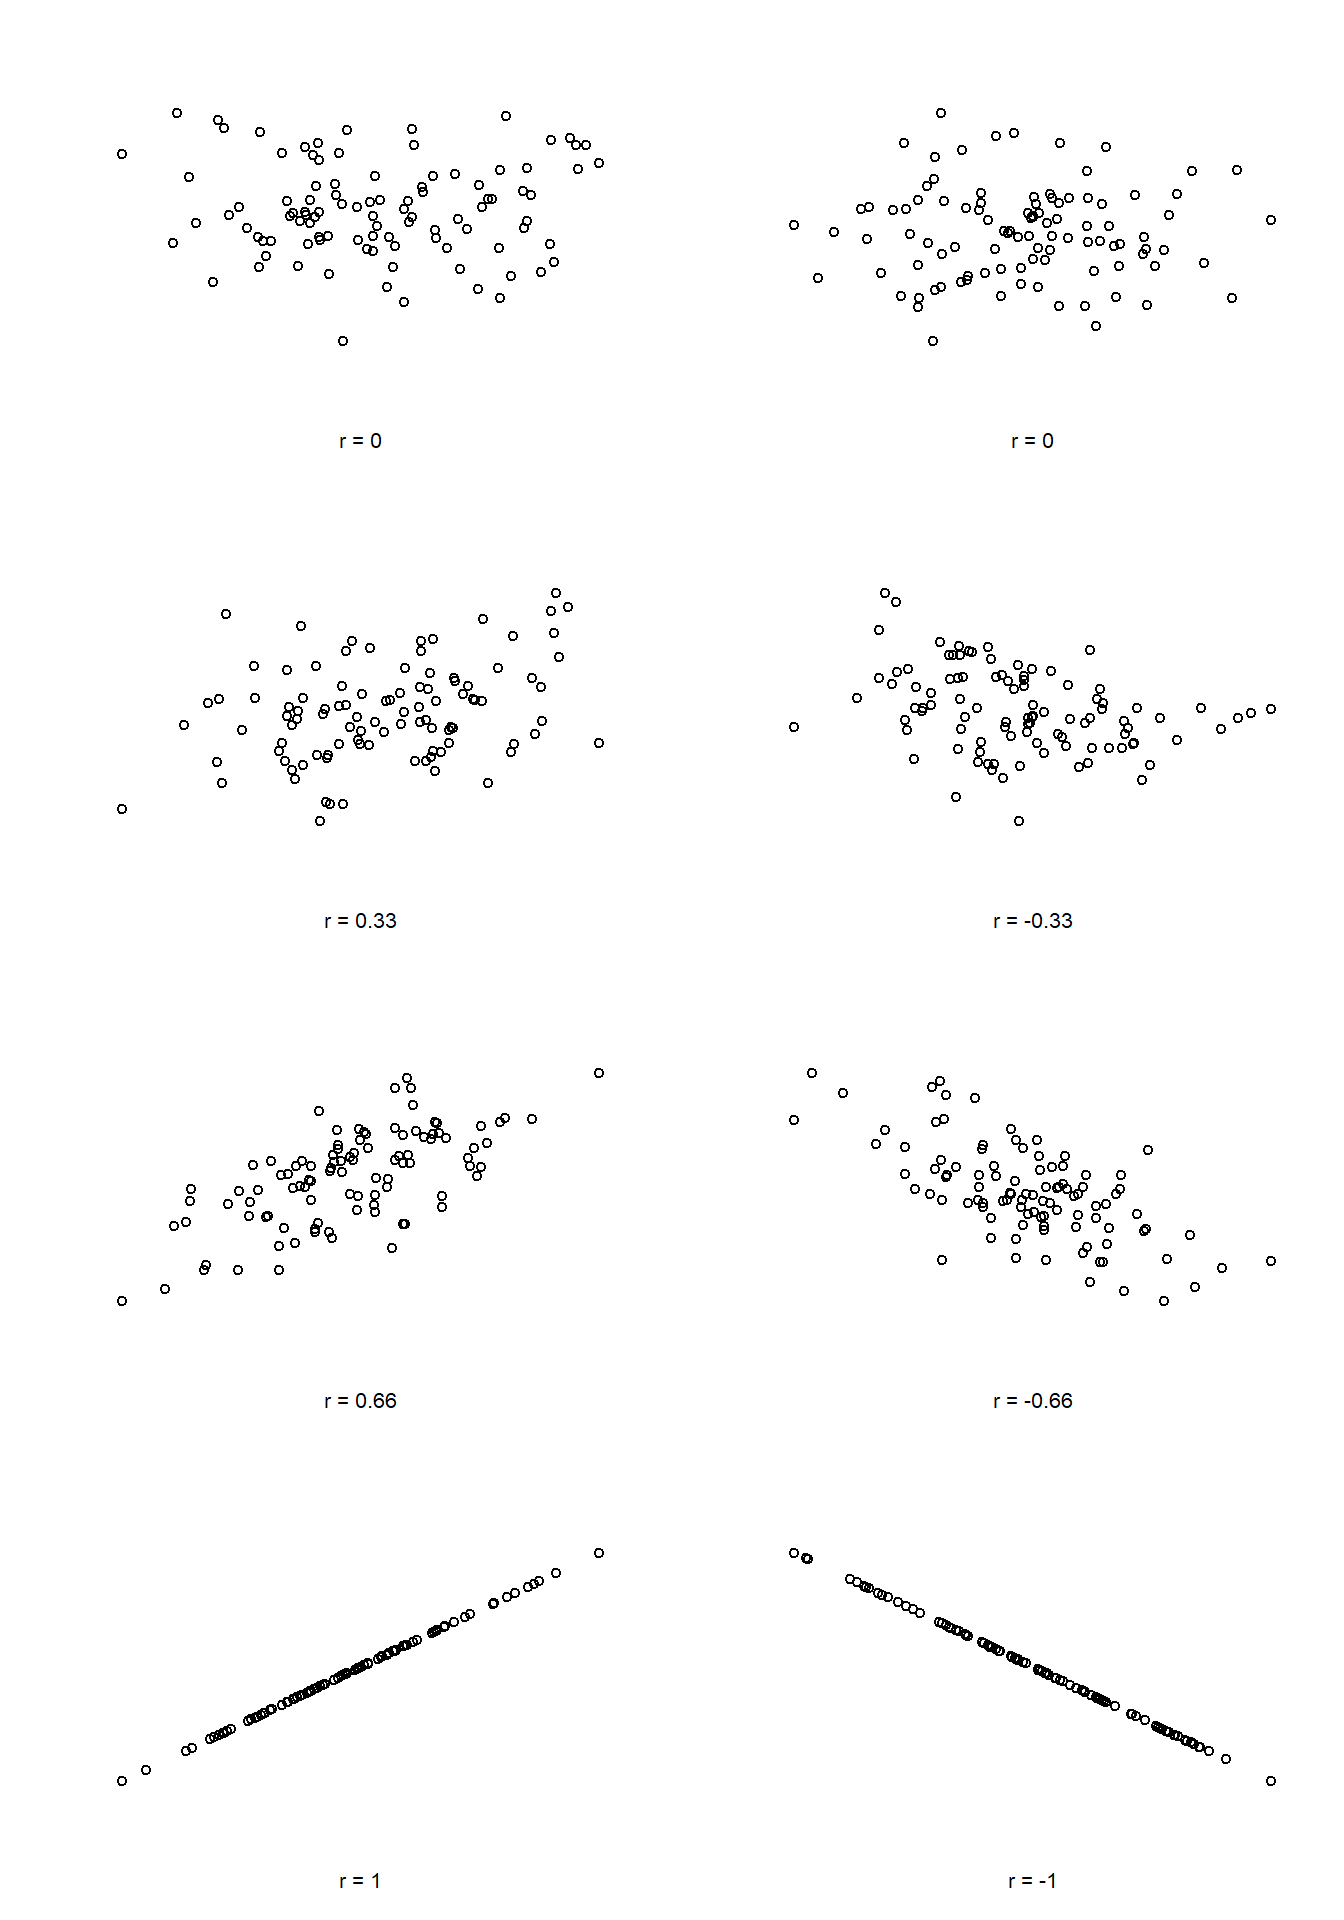
\includegraphics{./img/corr-1.png}
\caption{\label{fig:correlations}Different correlations.}
\end{figure}

In R, we can calculate the correlations of two variables using the \texttt{cor()} function. Consider the following example.

\begin{Shaded}
\begin{Highlighting}[]
\NormalTok{x }\OtherTok{\textless{}{-}} \DecValTok{1}\SpecialCharTok{:}\DecValTok{20}
\NormalTok{y }\OtherTok{\textless{}{-}}\NormalTok{ (x}\SpecialCharTok{\^{}}\DecValTok{2}\NormalTok{)}

\FunctionTok{ggplot}\NormalTok{(}\AttributeTok{data=}\ConstantTok{NULL}\NormalTok{, }\FunctionTok{aes}\NormalTok{(}\AttributeTok{x =}\NormalTok{ x, }\AttributeTok{y=}\NormalTok{y)) }\SpecialCharTok{+}
  \FunctionTok{geom\_point}\NormalTok{()}
\end{Highlighting}
\end{Shaded}

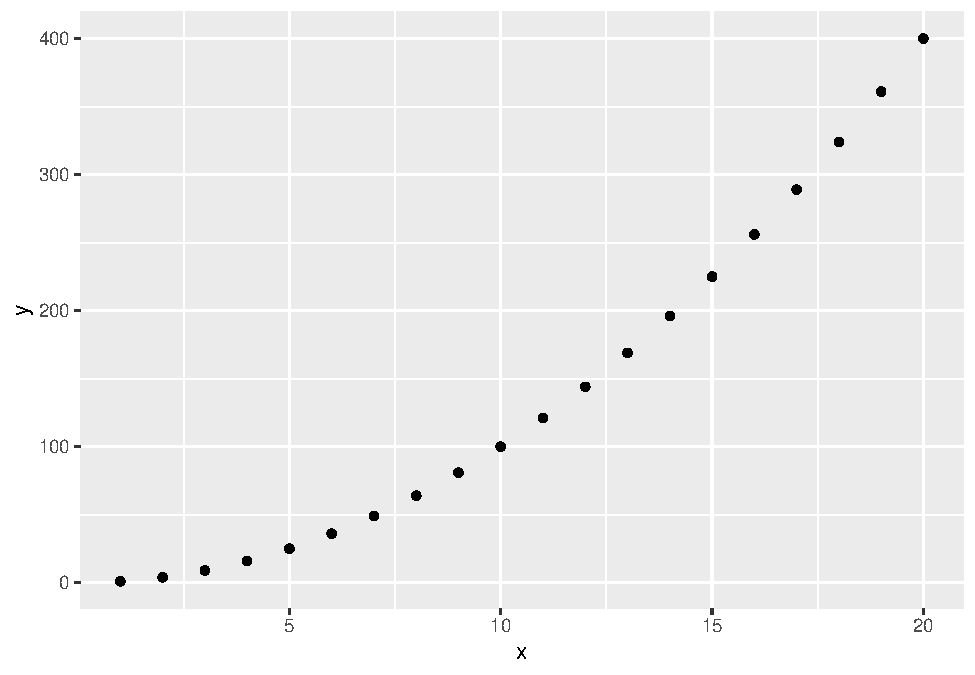
\includegraphics{main_files/figure-latex/unnamed-chunk-200-1.pdf}

\begin{Shaded}
\begin{Highlighting}[]
\FunctionTok{cor}\NormalTok{(x,y)}
\end{Highlighting}
\end{Shaded}

\begin{Shaded}
\begin{Highlighting}[]
\NormalTok{\#\# [1] 0.9713482}
\end{Highlighting}
\end{Shaded}

\hypertarget{linear-regression}{%
\chapter{Linear Regression}\label{linear-regression}}

In the previous section, we looked at some descriptive statistics about data. In all of these cases, we looked at the descriptive statistics of a \textbf{single variable}. For example, we looked at the mean and standard deviation of total sleep hours for various animals. The variable we considered was \texttt{total\_sleep\_hours}. This is also called \textbf{univariate statistics} because we were interested in the statistics of a \textbf{single variable}.

Now, we are moving onto \textbf{bivariate statistics}. In other words, we will analyze the relationship between two variables. Instead of calculating the \textbf{mean} of a single variable, we will calculate the \textbf{conditional mean} of a variable based on some other variable. For example, we could try calculating the relationship between \texttt{total\_sleep\_hours} and \texttt{bodyweight}.

\hypertarget{word-frequency-effects}{%
\section{Word Frequency Effects}\label{word-frequency-effects}}

Instead of looking at animal sleep hours, this time let's look at something more relevant for linguistics. Earlier, we discussed the role of frequency in processing.

\begin{itemize}
\tightlist
\item
  Our hypothesis was that more frequent words will be processed more easily.
\item
  We operationalized this hypothesis by picking

  \begin{itemize}
  \tightlist
  \item
    \textbf{word frequency} as our \textbf{independent variable} (also called a \textbf{predictor})
  \item
    \textbf{reaction time} as our \textbf{dependent variable} (also called \textbf{response} or \textbf{outcome variable})
  \end{itemize}
\end{itemize}

The typical dataset we will be working with has a structure similar to the one below:

\begin{longtable}[]{@{}
  >{\raggedright\arraybackslash}p{(\columnwidth - 6\tabcolsep) * \real{0.2174}}
  >{\raggedright\arraybackslash}p{(\columnwidth - 6\tabcolsep) * \real{0.2174}}
  >{\raggedright\arraybackslash}p{(\columnwidth - 6\tabcolsep) * \real{0.2609}}
  >{\raggedright\arraybackslash}p{(\columnwidth - 6\tabcolsep) * \real{0.3043}}@{}}
\toprule()
\begin{minipage}[b]{\linewidth}\raggedright
dependent var.(\(Y\))
\end{minipage} & \begin{minipage}[b]{\linewidth}\raggedright
predictor 1(\(X_1\))
\end{minipage} & \begin{minipage}[b]{\linewidth}\raggedright
predictor 2(\(X_2\))
\end{minipage} & \begin{minipage}[b]{\linewidth}\raggedright
(other predictors)
\end{minipage} \\
\midrule()
\endhead
705 & 1.2 & 2.2 & (\ldots) \\
209 & 8.3 & -4.0 & (\ldots) \\
334 & 7.2 & -1.4 & (\ldots) \\
\ldots{} & \ldots{} & \ldots{} & (\ldots) \\
\bottomrule()
\end{longtable}

\begin{itemize}
\tightlist
\item
  What the variables represent will depend on the problem you're studying and the question you're asking

  \begin{itemize}
  \tightlist
  \item
    dependent variable (e.g., reaction time)
  \item
    predictor 1 (e.g., frequency)
  \item
    predictor 2 (e.g., familiarity)
  \end{itemize}
\end{itemize}

Let us take a look at a linear regression model where \texttt{x\ =\ frequency} and \texttt{y=response\ time}.

\begin{figure}
\centering
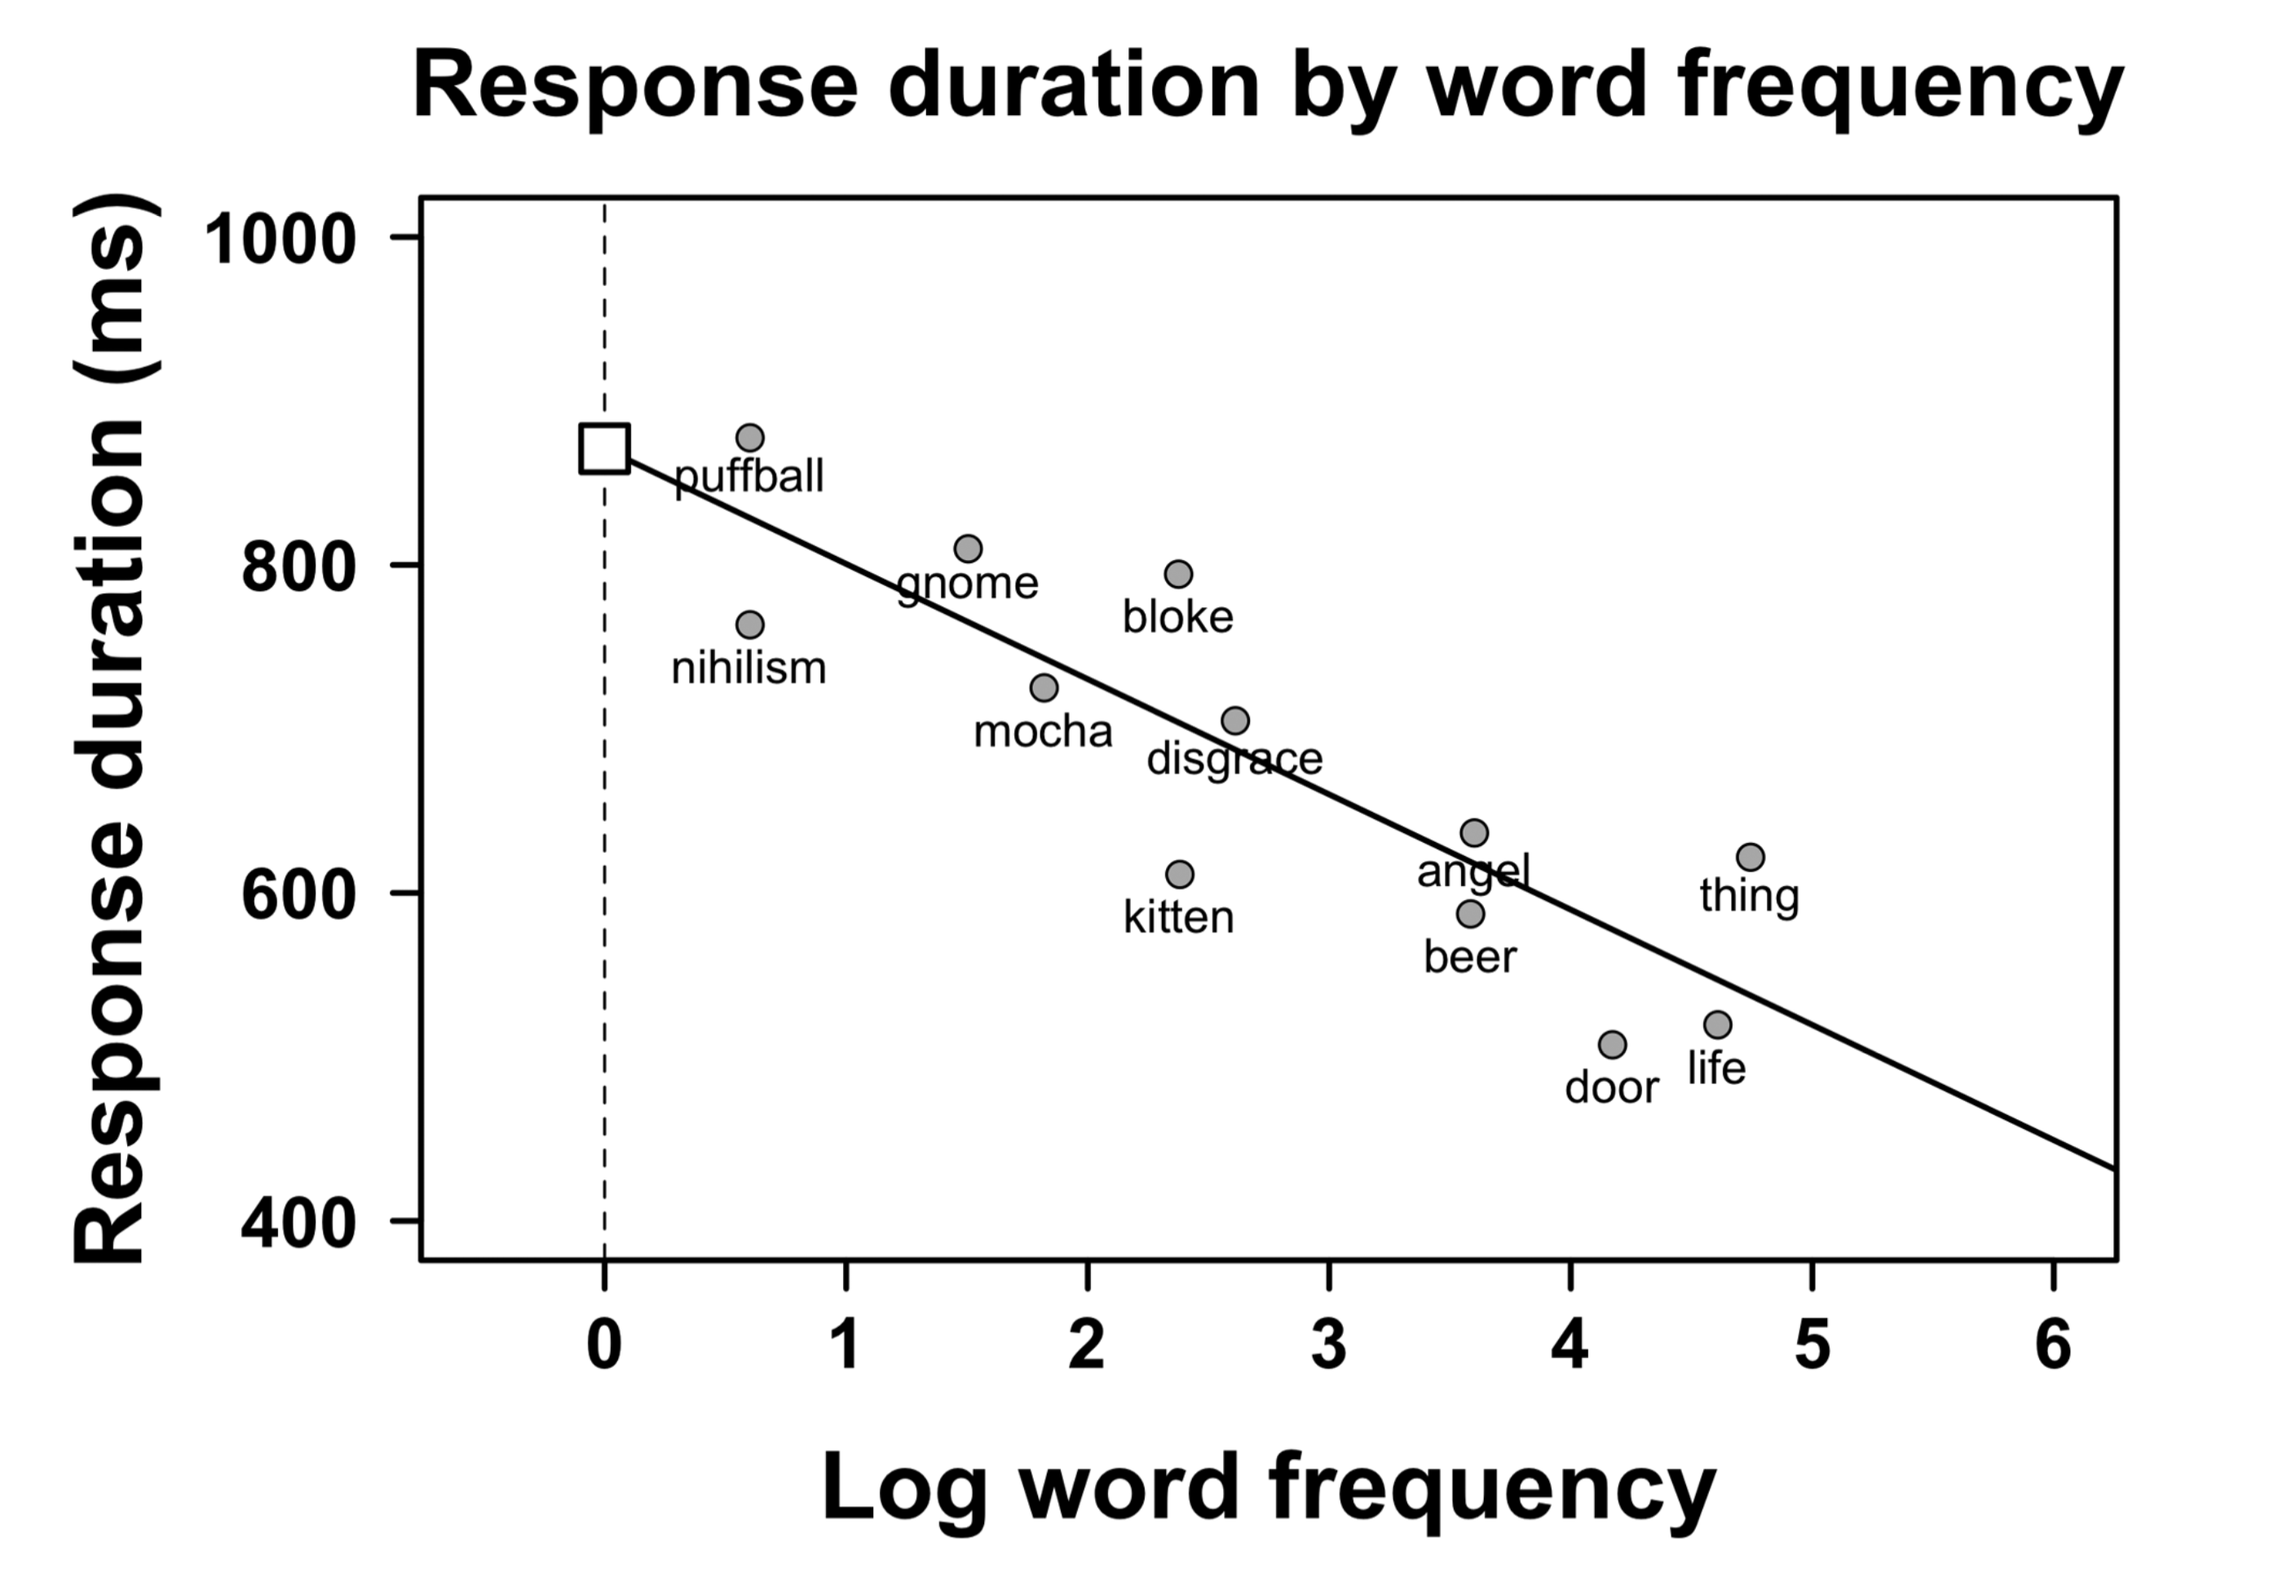
\includegraphics{./img/lr/lr1.png}
\caption{\label{fig:linearregression1}Response duration as a function of word frequency. The frequencies are not raw frequencies. Instead, log frequencies are used. We'll talk more about this.}
\end{figure}

\begin{itemize}
\tightlist
\item
  Each point on the plot above indicates the average response time of multiple participants.
\item
  The somewhat diagonal line is called the \textbf{regression line}.
\end{itemize}

\hypertarget{simple-linear-regression}{%
\section{Simple Linear Regression}\label{simple-linear-regression}}

In simple regression, our goal is to find the \textbf{regression line} as IT IS our model. The line extends to infinity and makes predictions about every point on its path. For example, our \textbf{model} can make a prediction about the reaction time if I were to find a word that has the log frequency 7. It would tell me that the reaction time would be a little below 400 miliseconds.

An important point regarding simple linear regression is that it can be used for data where the dependent variable is \textbf{continuous} (e.g.~436 miliseconds) but not \textbf{categorial} (e.g.~grammatical/ungrammatical).

\hypertarget{finding-the-regression-line}{%
\section{Finding the Regression Line}\label{finding-the-regression-line}}

In simple linear regression, the value for a \textbf{dependent variable} is a \textbf{linear function of} the \textbf{predictor variable}. A linear function looks like the following.

\[y = a + b * x\]

Let us try to understand these values a bit.

\[ \underbrace{Y}_{\text{dependent variable}} =
            \overbrace{\underbrace{a}_{\text{intercept}}}^{\text{additive term}} + 
            \overbrace{\underbrace{b}_{\text{slope}} * \underbrace{X}_{\text{predictor}}}^{\text{additive term}} \]

Mathematically, a line is defined in terms of an \textbf{intercept} and \textbf{slope}.

\begin{itemize}
\tightlist
\item
  \textbf{Slope} can be defined as the amount of change in \texttt{y} as \texttt{x} changes one unit.
  \[ slope = \frac{\Delta y}{\Delta x}  \]
\item
  A rising slope will have a positive value whereas a descending slope will have a positive value.
\item
  For example, the slope in the Response Duration Model above is -70. This means that for each unit of increase in frequency, we observe a 70ms decrease in reaction time.
\end{itemize}

A slope is not enough to define a line on a plot. There can be an infinite number of lines that have the same slope. We also need the \textbf{intercept}. Intercept determines the value predicted for y when x is 0. Consider the following graphs.

\begin{figure}
\centering
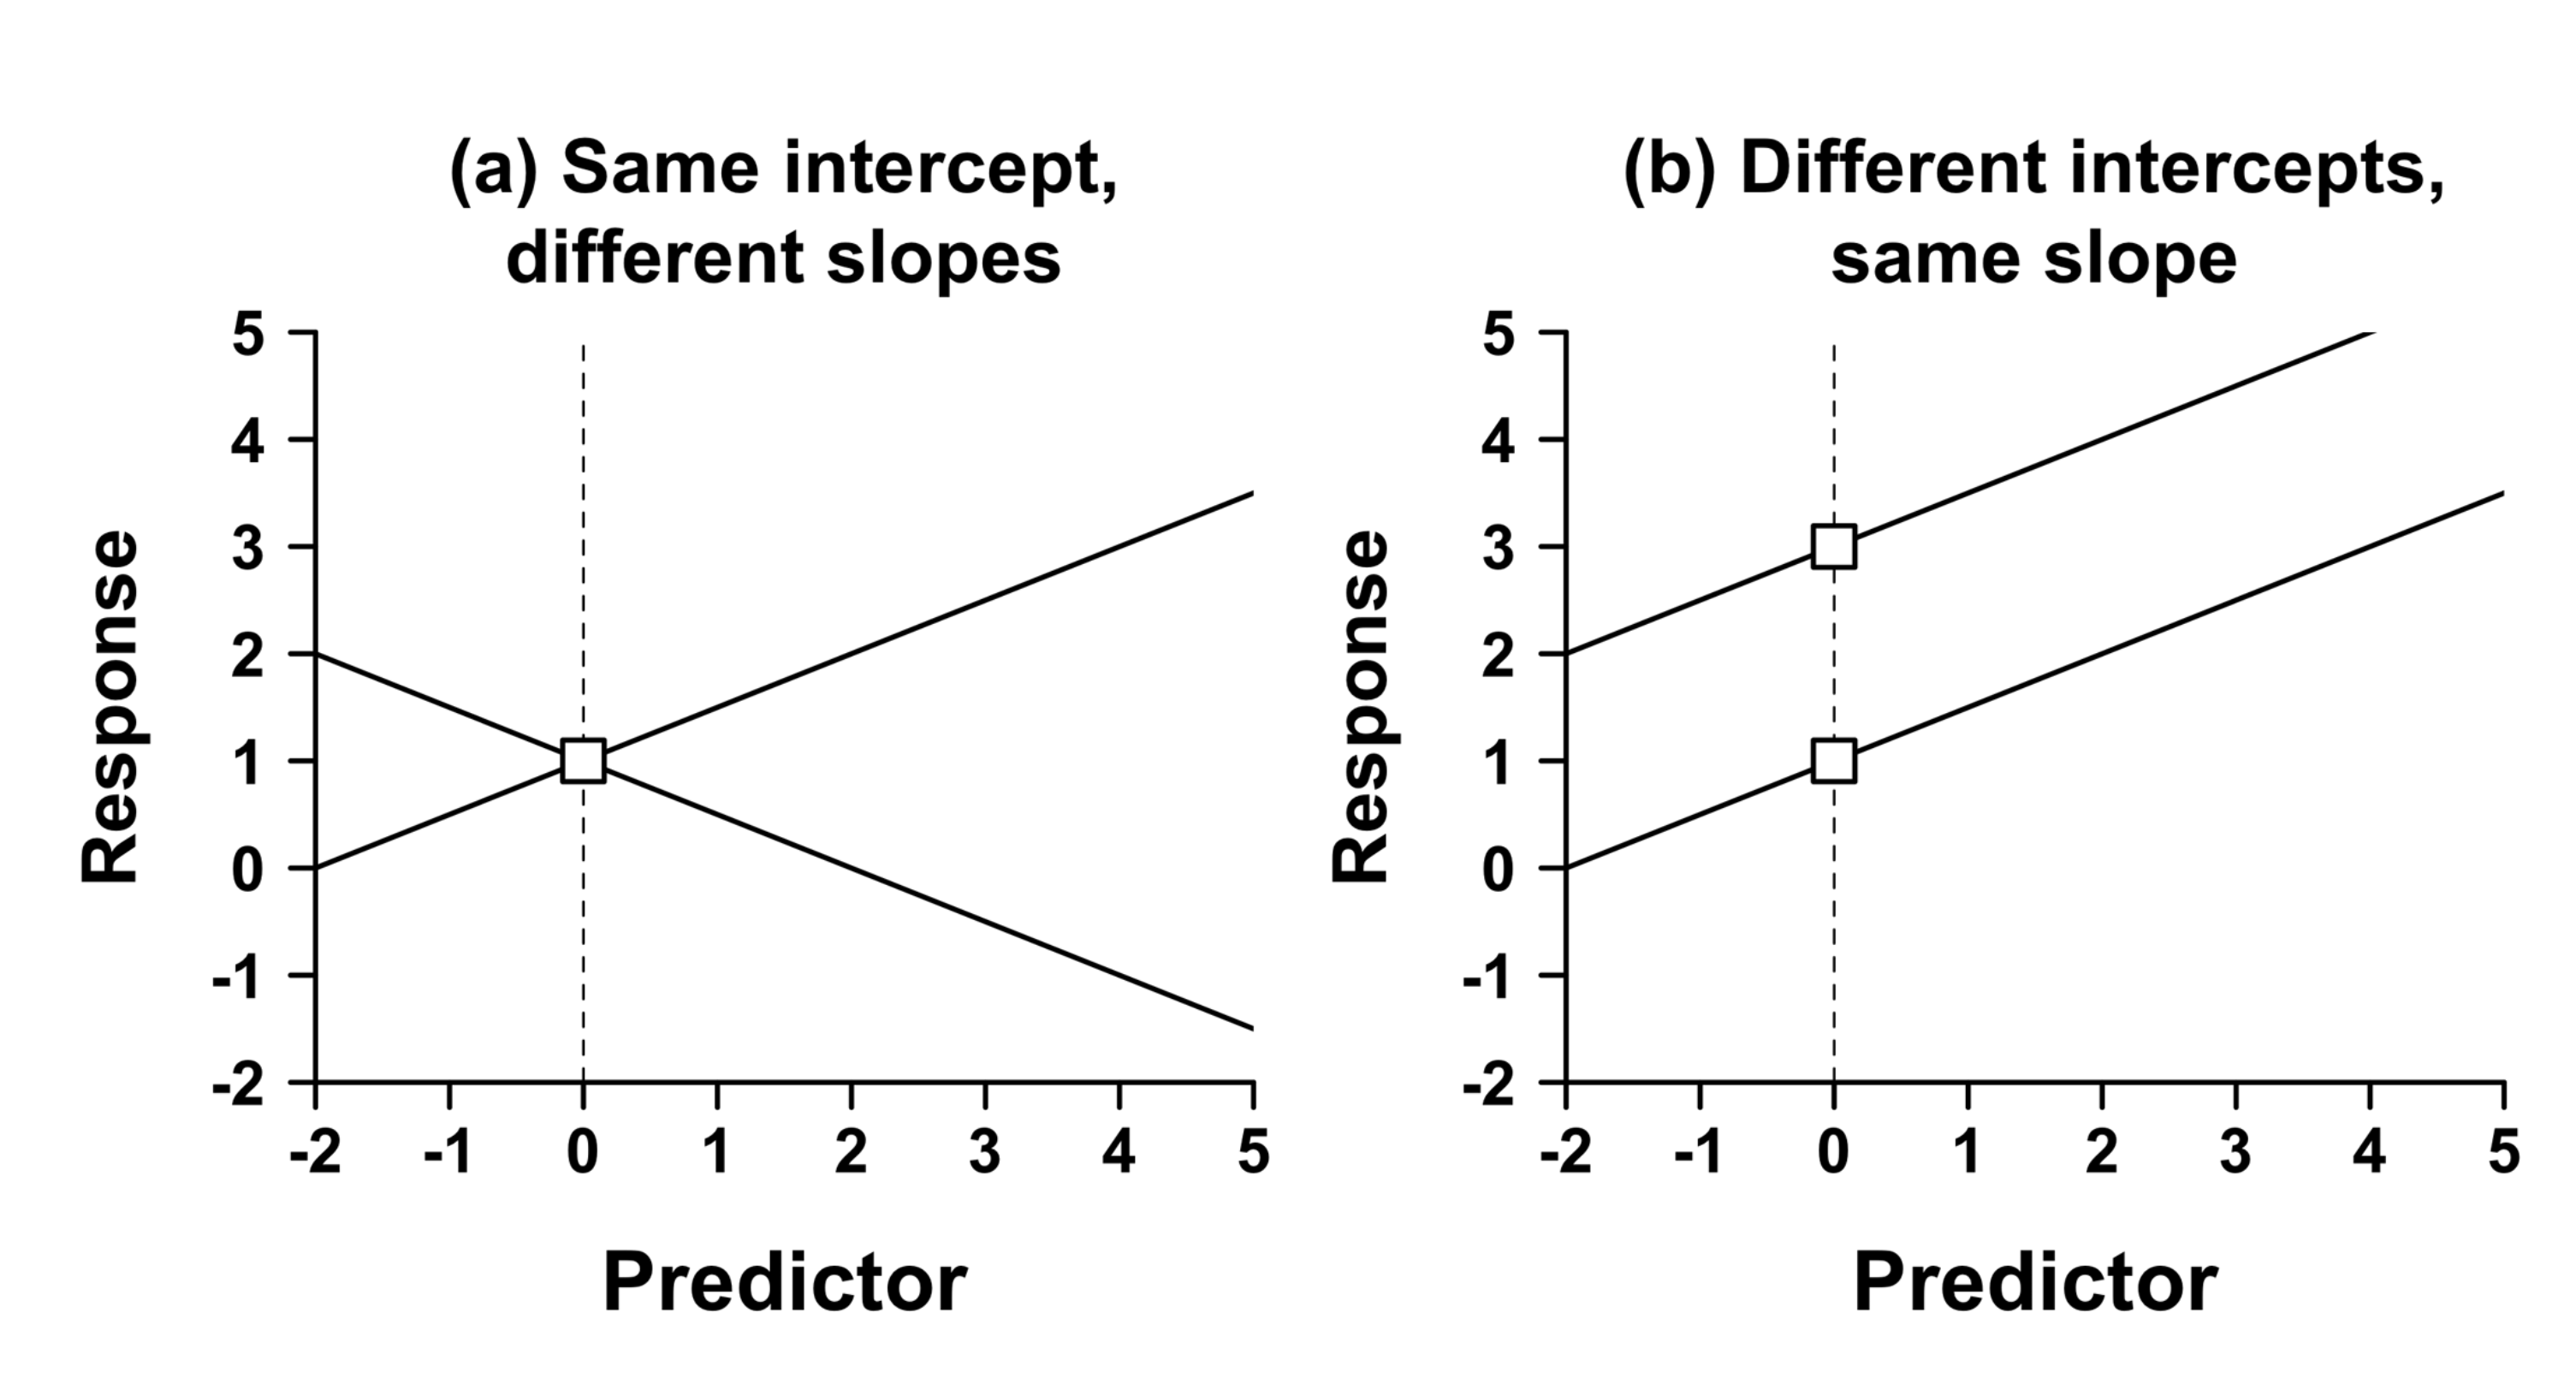
\includegraphics{./img/lr/lr2.png}
\caption{\label{fig:interceptslope}Lines with different intercept and slope values.}
\end{figure}

The intercept for the data Response Duration Model above is 880ms. So, our Response Duration Model is:

\[response\ duration = 880ms + (-70 \frac{ms}{freq}) * word\ frequecny   \]

A good way to remember the intercept and the slope and a linear model is to remember the \textbf{taxi fares}. The taxi fares will usually start with a constant fee (a minimum fee). This is your intercept. It's the 0th kilometers and it already costs you 7 TLs. Then the cost for each kilometer is your slope. At the time of writing these notes, it is 6TLs.

\begin{Shaded}
\begin{Highlighting}[]
\FunctionTok{library}\NormalTok{(ggplot2)}

\NormalTok{distance }\OtherTok{=} \DecValTok{1}\SpecialCharTok{:}\DecValTok{20}
\NormalTok{cost }\OtherTok{=} \DecValTok{7}\SpecialCharTok{+}\NormalTok{(}\DecValTok{6}\SpecialCharTok{*}\NormalTok{distance)}

\FunctionTok{ggplot}\NormalTok{(}\AttributeTok{data=}\ConstantTok{NULL}\NormalTok{, }\FunctionTok{aes}\NormalTok{(distance,cost)) }\SpecialCharTok{+}
  \FunctionTok{scale\_x\_continuous}\NormalTok{(}\AttributeTok{breaks =} \FunctionTok{seq}\NormalTok{(}\DecValTok{0}\NormalTok{, }\DecValTok{20}\NormalTok{, }\AttributeTok{by =}\DecValTok{1}\NormalTok{)) }\SpecialCharTok{+}
  \FunctionTok{scale\_y\_continuous}\NormalTok{(}\AttributeTok{breaks =} \FunctionTok{seq}\NormalTok{(}\DecValTok{0}\NormalTok{, }\DecValTok{125}\NormalTok{, }\AttributeTok{by =} \DecValTok{5}\NormalTok{)) }\SpecialCharTok{+} 
  \FunctionTok{geom\_smooth}\NormalTok{(}\AttributeTok{method=}\StringTok{"lm"}\NormalTok{, }\AttributeTok{formula =}\NormalTok{y}\SpecialCharTok{\textasciitilde{}}\NormalTok{x }\SpecialCharTok{+} \FunctionTok{I}\NormalTok{(}\DecValTok{7}\SpecialCharTok{+}\DecValTok{6}\SpecialCharTok{*}\NormalTok{x))}
\end{Highlighting}
\end{Shaded}

\begin{verbatim}
## Warning in predict.lm(model, newdata = new_data_frame(list(x = xseq)), se.fit =
## se, : prediction from a rank-deficient fit may be misleading
\end{verbatim}

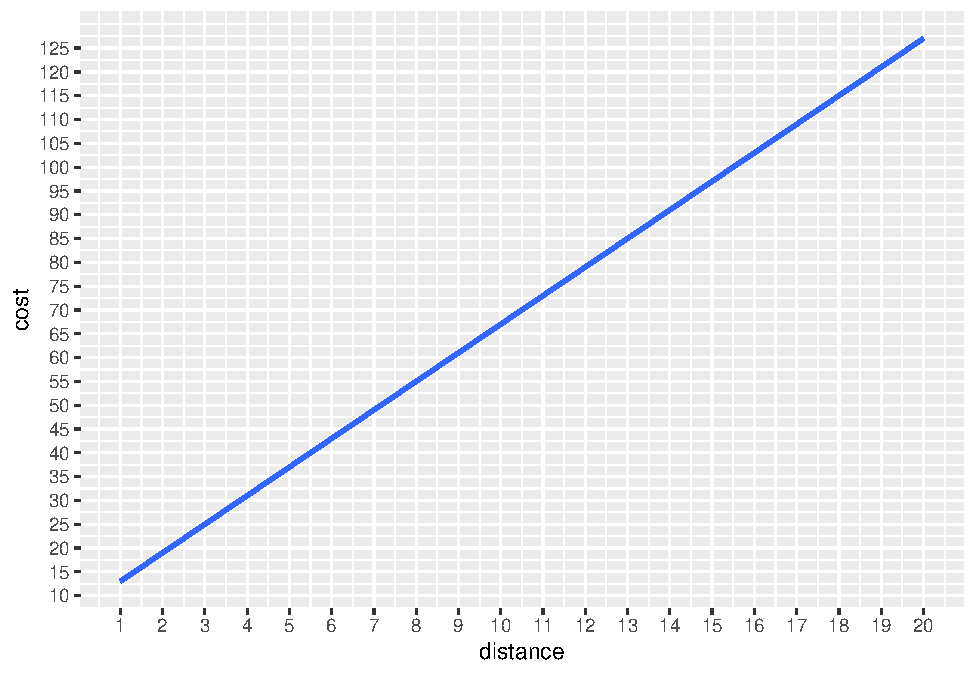
\includegraphics{main_files/figure-latex/unnamed-chunk-201-1.pdf}

\textbf{Slope} and \textbf{intercept} are the \textbf{coefficients} of our linear regression model. Our task is to find the \textbf{coefficients} from the data.

\hypertarget{estimating-the-coefficients}{%
\section{Estimating the Coefficients}\label{estimating-the-coefficients}}

A Linear Regression analysis of a particular data is essentially all about \textbf{estimating coefficients} and \textbf{interpreting the results}. In the \textbf{taxi model}, we already knew the coefficients. So, we had a model about the world and we can use the model to make predictions about taxi costs. In the Response Duration Model, the coefficients were learnt from the data but I gave them to you directly. So, how are we going to estimate the coefficients when what we have is just data but nothing else?

Let's not get into the weeds of how to find the right linear regression model. Instead, let's just use R to estimate the coefficients. This is called \textbf{fitting a model}. So, let's fit a linear model on the taxi model and interpret its results. We'll start with the taxi model simply because we already know the coefficients. We'll let R estimate some coefficients for us and then compare them with the coefficients we used to generate the \texttt{cost} data above from the \texttt{distance} variables and our coefficients.

The simplest way to fit a linear model on some data is the \texttt{lm()} function. \texttt{lm()} takes two variables \texttt{x} (predictor) and \texttt{y} (dependent variable) and fits a model by modeling \texttt{y} as a linear function of \texttt{x}. The tilde \texttt{\textasciitilde{}} means: element on the left as a function of element on the right.

For our taxi model, we will model cost as a function of duration. The following lines of code does that.

\begin{Shaded}
\begin{Highlighting}[]
\CommentTok{\# fit a linear regression model of cost as a function of distance}
\NormalTok{taxi\_model }\OtherTok{\textless{}{-}} \FunctionTok{lm}\NormalTok{(cost }\SpecialCharTok{\textasciitilde{}}\NormalTok{ distance)}

\CommentTok{\# print the model coefficients}
\NormalTok{taxi\_model}
\end{Highlighting}
\end{Shaded}

\begin{Shaded}
\begin{Highlighting}[]
\NormalTok{\#\# }
\NormalTok{\#\# Call:}
\NormalTok{\#\# lm(formula = cost \textasciitilde{} distance)}
\NormalTok{\#\# }
\NormalTok{\#\# Coefficients:}
\NormalTok{\#\# (Intercept)     distance  }
\NormalTok{\#\#           7            6}
\end{Highlighting}
\end{Shaded}

\textbf{Unbelievable!} The model estimated the intercept (start cost) as 7 and the slope (cost per km) as 6. Simple as that. Notice that the model estimated these coefficients simply from the data but nothing else.

The model object that we stored in the variable \texttt{taxi\_model} has a lot more information. Let us take a look at the results of our model. To do this, we'll take use the \texttt{glance()} function from the \texttt{broom} package.

\begin{Shaded}
\begin{Highlighting}[]
\FunctionTok{library}\NormalTok{(broom)}
\FunctionTok{library}\NormalTok{(tidyverse)}
\FunctionTok{glance}\NormalTok{(taxi\_model)}
\end{Highlighting}
\end{Shaded}

\begin{verbatim}
## Warning in summary.lm(x): essentially perfect fit: summary may be unreliable

## Warning in summary.lm(x): essentially perfect fit: summary may be unreliable
\end{verbatim}

\begin{Shaded}
\begin{Highlighting}[]
\NormalTok{\#\# \# A tibble: 1 x 12}
\NormalTok{\#\#   r.squ\textasciitilde{}1 adj.r\textasciitilde{}2    sigma stati\textasciitilde{}3   p.value    df logLik    AIC    BIC deviance}
\NormalTok{\#\#     \textless{}dbl\textgreater{}   \textless{}dbl\textgreater{}    \textless{}dbl\textgreater{}   \textless{}dbl\textgreater{}     \textless{}dbl\textgreater{} \textless{}dbl\textgreater{}  \textless{}dbl\textgreater{}  \textless{}dbl\textgreater{}  \textless{}dbl\textgreater{}    \textless{}dbl\textgreater{}}
\NormalTok{\#\# 1       1       1 4.66e{-}15 1.10e33 1.51e{-}287     1   633. {-}1259. {-}1256. 3.90e{-}28}
\NormalTok{\#\# \# ... with 2 more variables: df.residual \textless{}int\textgreater{}, nobs \textless{}int\textgreater{}, and abbreviated}
\NormalTok{\#\# \#   variable names 1: r.squared, 2: adj.r.squared, 3: statistic}
\end{Highlighting}
\end{Shaded}

There are a lot of details. For now, we'll focus on only two values \textbf{R2} and the \textbf{p value}.

\begin{Shaded}
\begin{Highlighting}[]
\NormalTok{results }\OtherTok{\textless{}{-}} \FunctionTok{glance}\NormalTok{(taxi\_model) }\SpecialCharTok{\%\textgreater{}\%}
  \FunctionTok{select}\NormalTok{(r.squared, p.value)}
\end{Highlighting}
\end{Shaded}

\begin{verbatim}
## Warning in summary.lm(x): essentially perfect fit: summary may be unreliable

## Warning in summary.lm(x): essentially perfect fit: summary may be unreliable
\end{verbatim}

\begin{Shaded}
\begin{Highlighting}[]
\NormalTok{results}
\end{Highlighting}
\end{Shaded}

\begin{Shaded}
\begin{Highlighting}[]
\NormalTok{\#\# \# A tibble: 1 x 2}
\NormalTok{\#\#   r.squared   p.value}
\NormalTok{\#\#       \textless{}dbl\textgreater{}     \textless{}dbl\textgreater{}}
\NormalTok{\#\# 1         1 1.51e{-}287}
\end{Highlighting}
\end{Shaded}

Without going into any detail yet, I can tell you that we got an excellent model. Our \textbf{R2} is 1, which is perfect and our p value is very small \texttt{1.51e-287} (This means that there are 286 zeroes after 0. and before 151. So, a very small number). When the p value is so small, we can conclude that the relation between distance and cost is \textbf{statistically significant} (i.e.~not random).

\hypertarget{data-is-messy}{%
\section{Data is messy}\label{data-is-messy}}

In the taxi model above, we worked with a very simplistic and ideal dataset. We know that in theory that is what a tax fare should look like. However, İstanbul is a crowded city and there are lots of traffic jams and traffic is quite unpredictable as there are so many random variables. Since the taxi charges you not only for the distance but also the duration you wait at the lights, there is always going to be some random addition to the fare. Let us incorporate that randomness to our taxi cost data and rerun our model to see what it looks like.

All we are going to do is to add some random values to our taxi prices. Let's generate some random numbers and bind it to a new cost variable.

\begin{Shaded}
\begin{Highlighting}[]
\NormalTok{hidden\_cost }\OtherTok{\textless{}{-}} \FunctionTok{rnorm}\NormalTok{(}\DecValTok{20}\NormalTok{, }\AttributeTok{mean=}\FloatTok{7.5}\NormalTok{, }\AttributeTok{sd=}\FloatTok{4.5}\NormalTok{)}
\NormalTok{total\_cost }\OtherTok{\textless{}{-}}\NormalTok{ cost }\SpecialCharTok{+}\NormalTok{ hidden\_cost}
\end{Highlighting}
\end{Shaded}

Let us plot the theoretical costs and the total costs side by side. We'll use the \texttt{gridExtra} package to plot two plots side by side.

\begin{Shaded}
\begin{Highlighting}[]
\FunctionTok{library}\NormalTok{(gridExtra)}
\end{Highlighting}
\end{Shaded}

\begin{verbatim}
## 
## Attaching package: 'gridExtra'
\end{verbatim}

\begin{verbatim}
## The following object is masked from 'package:dplyr':
## 
##     combine
\end{verbatim}

\begin{Shaded}
\begin{Highlighting}[]
\NormalTok{plot1 }\OtherTok{\textless{}{-}} \FunctionTok{ggplot}\NormalTok{(}\AttributeTok{data=}\ConstantTok{NULL}\NormalTok{, }\FunctionTok{aes}\NormalTok{(distance,cost)) }\SpecialCharTok{+}
  \FunctionTok{scale\_x\_continuous}\NormalTok{(}\AttributeTok{breaks =} \FunctionTok{seq}\NormalTok{(}\DecValTok{0}\NormalTok{, }\DecValTok{20}\NormalTok{, }\AttributeTok{by =}\DecValTok{1}\NormalTok{)) }\SpecialCharTok{+}
  \FunctionTok{scale\_y\_continuous}\NormalTok{(}\AttributeTok{breaks =} \FunctionTok{seq}\NormalTok{(}\DecValTok{0}\NormalTok{, }\DecValTok{125}\NormalTok{, }\AttributeTok{by =} \DecValTok{5}\NormalTok{)) }\SpecialCharTok{+} 
  \FunctionTok{geom\_smooth}\NormalTok{(}\AttributeTok{method=}\StringTok{"lm"}\NormalTok{) }\SpecialCharTok{+}
  \FunctionTok{geom\_point}\NormalTok{() }\SpecialCharTok{+}
  \FunctionTok{ggtitle}\NormalTok{(}\StringTok{"Taxi cost without traffic"}\NormalTok{)}

\NormalTok{plot2 }\OtherTok{\textless{}{-}} \FunctionTok{ggplot}\NormalTok{(}\AttributeTok{data=}\ConstantTok{NULL}\NormalTok{, }\FunctionTok{aes}\NormalTok{(distance,total\_cost)) }\SpecialCharTok{+}
  \FunctionTok{scale\_x\_continuous}\NormalTok{(}\AttributeTok{breaks =} \FunctionTok{seq}\NormalTok{(}\DecValTok{0}\NormalTok{, }\DecValTok{20}\NormalTok{, }\AttributeTok{by =}\DecValTok{1}\NormalTok{)) }\SpecialCharTok{+}
  \FunctionTok{scale\_y\_continuous}\NormalTok{(}\AttributeTok{breaks =} \FunctionTok{seq}\NormalTok{(}\DecValTok{0}\NormalTok{, }\DecValTok{125}\NormalTok{, }\AttributeTok{by =} \DecValTok{5}\NormalTok{)) }\SpecialCharTok{+} 
  \FunctionTok{geom\_smooth}\NormalTok{(}\AttributeTok{method=}\StringTok{"lm"}\NormalTok{)}\SpecialCharTok{+}
  \FunctionTok{geom\_point}\NormalTok{()}\SpecialCharTok{+}
  \FunctionTok{ggtitle}\NormalTok{(}\StringTok{"Taxi cost with traffic"}\NormalTok{)}

\FunctionTok{grid.arrange}\NormalTok{(plot1, plot2, }\AttributeTok{ncol=}\DecValTok{2}\NormalTok{)}
\end{Highlighting}
\end{Shaded}

\begin{verbatim}
## `geom_smooth()` using formula 'y ~ x'
\end{verbatim}

\begin{verbatim}
## `geom_smooth()` using formula 'y ~ x'
\end{verbatim}

\includegraphics{main_files/figure-latex/unnamed-chunk-206-1.pdf}

OK, now it looks like we have some more realistic data. Let us rerun our linear model to see what the coefficients look like.

\begin{Shaded}
\begin{Highlighting}[]
\NormalTok{better\_taxi\_model }\OtherTok{\textless{}{-}} \FunctionTok{lm}\NormalTok{(total\_cost}\SpecialCharTok{\textasciitilde{}}\NormalTok{distance)}

\NormalTok{better\_taxi\_model}
\end{Highlighting}
\end{Shaded}

\begin{Shaded}
\begin{Highlighting}[]
\NormalTok{\#\# }
\NormalTok{\#\# Call:}
\NormalTok{\#\# lm(formula = total\_cost \textasciitilde{} distance)}
\NormalTok{\#\# }
\NormalTok{\#\# Coefficients:}
\NormalTok{\#\# (Intercept)     distance  }
\NormalTok{\#\#      14.838        5.916}
\end{Highlighting}
\end{Shaded}

Notice that we got a new intercept and slope. It's kinda weird. We know that the taxi start fare is 7TL. However, our intercept is a lot higher (this will differ as each time you run your code as the traffic cost we calculated is random). In a few instances where I ran the model I got a number between 14-18. This is quite off given our original intercept.

Notice that the slope is a little off too. It's not exactly 6 but it's not way off like the intercept. So, did our linear model do well? Before answering this question more formally, I'll draw your attention to one point. Our model predicts that your initial taxi fare will be a little higher at the beginning and it will sort of even out as your distance increases. Even though our model doesn't guess the intercept correctly, it still does a very decent job in modeling the real life taxi costs (or a simulation of it). Just add up the intercept and slope and that should give you around the minimum cost you'll pay for a taxi ride.

\begin{Shaded}
\begin{Highlighting}[]
\FunctionTok{coef}\NormalTok{(better\_taxi\_model)[}\DecValTok{1}\NormalTok{] }\SpecialCharTok{+} \FunctionTok{coef}\NormalTok{(better\_taxi\_model)[}\DecValTok{2}\NormalTok{]}
\end{Highlighting}
\end{Shaded}

\begin{Shaded}
\begin{Highlighting}[]
\NormalTok{\#\# (Intercept) }
\NormalTok{\#\#    20.75445}
\end{Highlighting}
\end{Shaded}

At this point, I want to remind you that taxi rides in İstanbul have a minimum of 20TLs for short distance trips (2km or less). So, our model does pretty good for a real life scenario.

\hypertarget{simplified-frequency-data}{%
\section{Simplified Frequency Data}\label{simplified-frequency-data}}

Let us use a simple frequency data. Go ahead and download the \texttt{log10ELP\_frequency.csv} file from Moodle. This is the sam data in Bodo Winter's ELP\_frequency.csv file with an added column for log10 normalization. We will plot the data using a scatterplot with geom\_point and also draw a regression line.

We will use log normal values as the x axis and the reaction time as the y axis.

\begin{Shaded}
\begin{Highlighting}[]
\FunctionTok{library}\NormalTok{(ggrepel)}


\NormalTok{freq\_data }\OtherTok{\textless{}{-}} \FunctionTok{read\_csv}\NormalTok{(}\StringTok{"/Users/umit/Desktop/log10ELP\_frequency.csv"}\NormalTok{)}
\end{Highlighting}
\end{Shaded}

\begin{verbatim}
## Rows: 12 Columns: 4
## -- Column specification --------------------------------------------------------
## Delimiter: ","
## chr (1): Word
## dbl (3): RT, Freq, log10freq
## 
## i Use `spec()` to retrieve the full column specification for this data.
## i Specify the column types or set `show_col_types = FALSE` to quiet this message.
\end{verbatim}

\begin{Shaded}
\begin{Highlighting}[]
\FunctionTok{ggplot}\NormalTok{(freq\_data, }\FunctionTok{aes}\NormalTok{(}\AttributeTok{x=}\NormalTok{log10freq, }\AttributeTok{y=}\NormalTok{RT)) }\SpecialCharTok{+}
  \FunctionTok{scale\_x\_continuous}\NormalTok{(}\AttributeTok{limits =} \FunctionTok{c}\NormalTok{(}\DecValTok{0}\NormalTok{,}\DecValTok{5}\NormalTok{)) }\SpecialCharTok{+}
  \FunctionTok{geom\_text\_repel}\NormalTok{(}\FunctionTok{aes}\NormalTok{(}\AttributeTok{label =}\NormalTok{ Word)) }\SpecialCharTok{+}
  \FunctionTok{geom\_point}\NormalTok{()}\SpecialCharTok{+}
  \FunctionTok{geom\_smooth}\NormalTok{(}\AttributeTok{method=}\StringTok{"lm"}\NormalTok{,}\AttributeTok{se=}\NormalTok{F)}
\end{Highlighting}
\end{Shaded}

\begin{verbatim}
## `geom_smooth()` using formula 'y ~ x'
\end{verbatim}

\includegraphics{main_files/figure-latex/unnamed-chunk-209-1.pdf}

\begin{Shaded}
\begin{Highlighting}[]
\NormalTok{freq\_model }\OtherTok{\textless{}{-}} \FunctionTok{lm}\NormalTok{(freq\_data}\SpecialCharTok{$}\NormalTok{RT }\SpecialCharTok{\textasciitilde{}}\NormalTok{ freq\_data}\SpecialCharTok{$}\NormalTok{log10freq)}
\end{Highlighting}
\end{Shaded}

OK, let us also get a glace at our model. We'll first take a look at the slope and the intercept and then \textbf{R2} and the \textbf{p value}.

\begin{Shaded}
\begin{Highlighting}[]
\FunctionTok{coef}\NormalTok{(freq\_model)}
\end{Highlighting}
\end{Shaded}

\begin{Shaded}
\begin{Highlighting}[]
\NormalTok{\#\#         (Intercept) freq\_data$log10freq }
\NormalTok{\#\#           870.90539           {-}70.27646}
\end{Highlighting}
\end{Shaded}

\begin{Shaded}
\begin{Highlighting}[]
\FunctionTok{glance}\NormalTok{(freq\_model)}
\end{Highlighting}
\end{Shaded}

\begin{Shaded}
\begin{Highlighting}[]
\NormalTok{\#\# \# A tibble: 1 x 12}
\NormalTok{\#\#   r.squ\textasciitilde{}1 adj.r\textasciitilde{}2 sigma stati\textasciitilde{}3 p.value    df logLik   AIC   BIC devia\textasciitilde{}4 df.re\textasciitilde{}5}
\NormalTok{\#\#     \textless{}dbl\textgreater{}   \textless{}dbl\textgreater{} \textless{}dbl\textgreater{}   \textless{}dbl\textgreater{}   \textless{}dbl\textgreater{} \textless{}dbl\textgreater{}  \textless{}dbl\textgreater{} \textless{}dbl\textgreater{} \textless{}dbl\textgreater{}   \textless{}dbl\textgreater{}   \textless{}int\textgreater{}}
\NormalTok{\#\# 1   0.737   0.711  63.3    28.1 3.48e{-}4     1  {-}65.7  137.  139.  40115.      10}
\NormalTok{\#\# \# ... with 1 more variable: nobs \textless{}int\textgreater{}, and abbreviated variable names}
\NormalTok{\#\# \#   1: r.squared, 2: adj.r.squared, 3: statistic, 4: deviance, 5: df.residual}
\end{Highlighting}
\end{Shaded}

\hypertarget{residuals}{%
\section{Residuals}\label{residuals}}

So far, we built and plotted linear models by estimating the intercept and slope of a line that seems to best describe our data. In the simple taxi model, we were in a perfect position. Our model had a \textbf{perfect fit} on our data. However, once we introduced some \textbf{random noise} (e.g.~random traffic jams) into our data, our linear model still did a decent job but it was not a perfect fit.

Next, we tried modeling the simple frequency data and we got a decent model that describes the trend in our data but the fit is not perfect. Can we find a way to quantify how good our model fits our data (``goodness of fit''). That's what we will do here. Let us reconsider the frequency data plot. This time, we'll draw lines from the data points to the regression line. The distance for each data point is called a \textbf{residual}. It describes the amount by which our model missed the actual value.

\begin{Shaded}
\begin{Highlighting}[]
\NormalTok{freq\_model }\OtherTok{\textless{}{-}} \FunctionTok{lm}\NormalTok{(freq\_data}\SpecialCharTok{$}\NormalTok{RT }\SpecialCharTok{\textasciitilde{}}\NormalTok{ freq\_data}\SpecialCharTok{$}\NormalTok{log10freq)}
\FunctionTok{ggplot}\NormalTok{(freq\_data, }\FunctionTok{aes}\NormalTok{(}\AttributeTok{x=}\NormalTok{log10freq, }\AttributeTok{y=}\NormalTok{RT)) }\SpecialCharTok{+}
  \FunctionTok{scale\_x\_continuous}\NormalTok{(}\AttributeTok{limits =} \FunctionTok{c}\NormalTok{(}\DecValTok{0}\NormalTok{,}\DecValTok{5}\NormalTok{)) }\SpecialCharTok{+}
  \FunctionTok{geom\_text\_repel}\NormalTok{(}\FunctionTok{aes}\NormalTok{(}\AttributeTok{label =}\NormalTok{ Word)) }\SpecialCharTok{+}
  \FunctionTok{geom\_point}\NormalTok{()}\SpecialCharTok{+}
  \FunctionTok{geom\_smooth}\NormalTok{(}\AttributeTok{method=}\StringTok{"lm"}\NormalTok{,}\AttributeTok{se=}\NormalTok{F)}\SpecialCharTok{+}
  \FunctionTok{geom\_segment}\NormalTok{(}\FunctionTok{aes}\NormalTok{(}\AttributeTok{x =}\NormalTok{ log10freq, }\AttributeTok{y =}\NormalTok{ RT,}
                   \AttributeTok{xend =}\NormalTok{ log10freq, }\AttributeTok{yend =} \FunctionTok{fitted}\NormalTok{(freq\_model)))}
\end{Highlighting}
\end{Shaded}

\begin{verbatim}
## `geom_smooth()` using formula 'y ~ x'
\end{verbatim}

\includegraphics{main_files/figure-latex/unnamed-chunk-212-1.pdf}

\begin{Shaded}
\begin{Highlighting}[]
\FunctionTok{ggplot}\NormalTok{(freq\_data, }\FunctionTok{aes}\NormalTok{(}\AttributeTok{x=}\NormalTok{log10freq, }\AttributeTok{y=}\NormalTok{RT)) }\SpecialCharTok{+}
  \FunctionTok{scale\_x\_continuous}\NormalTok{(}\AttributeTok{limits =} \FunctionTok{c}\NormalTok{(}\DecValTok{0}\NormalTok{,}\DecValTok{5}\NormalTok{)) }\SpecialCharTok{+}
  \FunctionTok{geom\_text\_repel}\NormalTok{(}\FunctionTok{aes}\NormalTok{(}\AttributeTok{label =}\NormalTok{ Word)) }\SpecialCharTok{+}
  \FunctionTok{geom\_point}\NormalTok{()}\SpecialCharTok{+}
  \FunctionTok{geom\_hline}\NormalTok{(}\AttributeTok{yintercept =} \DecValTok{680}\NormalTok{)}\SpecialCharTok{+}
  \FunctionTok{geom\_segment}\NormalTok{(}\FunctionTok{aes}\NormalTok{(}\AttributeTok{x =}\NormalTok{ log10freq, }\AttributeTok{y =}\NormalTok{ RT,}
                   \AttributeTok{xend =}\NormalTok{ log10freq, }\AttributeTok{yend =} \DecValTok{700}\NormalTok{))}
\end{Highlighting}
\end{Shaded}

\includegraphics{main_files/figure-latex/unnamed-chunk-213-1.pdf}

Now, we have two models:

\begin{itemize}
\tightlist
\item
  A model where there is a relation between frequency and reaction time
\item
  A null model where there is no relation between frequency and reaction time (reaction time is independent of frequency)
\end{itemize}

\hypertarget{sum-of-squared-errors}{%
\subsection{Sum of Squared Errors}\label{sum-of-squared-errors}}

One way to describe the errors of the model is to sum the squares of each error value. This is called the Sum of Squared Errors.

To do this, we need to get the residuals of the model, square them and then sum them. Let us do this for the linear model.

\begin{Shaded}
\begin{Highlighting}[]
\NormalTok{SSE\_freq\_model }\OtherTok{\textless{}{-}} \FunctionTok{sum}\NormalTok{((}\FunctionTok{residuals}\NormalTok{(freq\_model))}\SpecialCharTok{\^{}}\DecValTok{2}\NormalTok{)}
\NormalTok{SSE\_freq\_model}
\end{Highlighting}
\end{Shaded}

\begin{Shaded}
\begin{Highlighting}[]
\NormalTok{\#\# [1] 40114.97}
\end{Highlighting}
\end{Shaded}

Let us also calculate it for the null model. The intercept for the null model was 680 I found this value by taking the average reaction time. This will be my null model. The mean was 679.9167. So, we'll deduce the the mean from the actual values to find the residuals. The rest is just the same.

\begin{Shaded}
\begin{Highlighting}[]
\NormalTok{null\_model\_residuals }\OtherTok{\textless{}{-}}\NormalTok{ freq\_data}\SpecialCharTok{$}\NormalTok{RT }\SpecialCharTok{{-}} \DecValTok{680}
\NormalTok{SSE\_null\_model }\OtherTok{\textless{}{-}} \FunctionTok{sum}\NormalTok{(null\_model\_residuals}\SpecialCharTok{\^{}}\DecValTok{2}\NormalTok{)}
\NormalTok{SSE\_null\_model}
\end{Highlighting}
\end{Shaded}

\begin{Shaded}
\begin{Highlighting}[]
\NormalTok{\#\# [1] 152743.3}
\end{Highlighting}
\end{Shaded}

These numbers are very similar to what Bodo Winter reports in his chapter. He might not have done the rounding I did. We use the null model to calculate a \textbf{standardized measure of fit}. One measure is \textbf{R2} and it is calculated as follows.

\[R^2 = 1 - \frac{SSE_{model}}{SSE_{null}} \]
Let's calculate \textbf{R2}.

\begin{Shaded}
\begin{Highlighting}[]
\NormalTok{r\_squared }\OtherTok{\textless{}{-}} \DecValTok{1} \SpecialCharTok{{-}}\NormalTok{ (SSE\_freq\_model}\SpecialCharTok{/}\NormalTok{SSE\_null\_model)}

\NormalTok{r\_squared}
\end{Highlighting}
\end{Shaded}

\begin{Shaded}
\begin{Highlighting}[]
\NormalTok{\#\# [1] 0.73737}
\end{Highlighting}
\end{Shaded}

\textbf{Excellent!} We've calculated \textbf{R2} and it is the same as what we found earlier when we took at a look at the model report using the \texttt{glance()} function.

So, what is this \textbf{R2}? When we interpret \textbf{R2}, we say ``n'' amount of the variance in the dependent variable (RT) can be accounted for by incorporating the independent variable (word frequency). In this case, 73\% of the variance is due to word frequency. The remaining 27\% is due to chance or some other factors we didn't consider.

  \bibliography{book.bib,packages.bib}

\end{document}
